\documentclass{article}


\usepackage{arxiv}

\usepackage[utf8]{inputenc} % allow utf-7 input
\usepackage[T1]{fontenc}    % use 8-bit T1 fonts
\usepackage{hyperref}       % hyperlinks
\usepackage{url}            % simple URL typesetting
\usepackage{booktabs}       % professional-quality tables
\usepackage{amsfonts}       % blackboard math symbols
\usepackage{nicefrac}       % compact symbols for 1/2, etc.
\usepackage{microtype}      % microtypography
\usepackage{lipsum}
\usepackage{graphicx}
\graphicspath{ {./images/} }

\usepackage{amsmath}
\usepackage{lmodern}%
\usepackage{textcomp}%
\usepackage{lastpage}%
% \usepackage[margin=0.5in]{geometry}%
\usepackage{float}%
\usepackage{xcolor}
\usepackage[export]{adjustbox}
\usepackage[numbers]{natbib}
\usepackage{listings}
\usepackage{minted}
\usemintedstyle{vs}
\usepackage{subfig}
\usepackage{multirow}
\usepackage{longtable}
\usepackage{authblk}
\usepackage{lscape}
\usepackage{array}

\captionsetup[table]{skip=10pt}



\renewcommand{\arraystretch}{1.5}

%Custom column type for better image-embedding
\newcolumntype{V}{>{\centering\arraybackslash} m{1.0cm} }



\begin{document}
\title{Machine Learning for Metallurgy I. A Neural Network Potential for Al-Cu}

\author[1]{Daniel Marchand}
\author[1]{Abhinav Jain}
\author[1]{Albert Glensk}
\author[1]{W. A. Curtin}
\affil[1]{Institute of Mechanical Engineering, École Polytechnique Fédérale de Lausanne, CH-1015, Vaud, Switzerland}

\maketitle

%\author{
% Daniel Marchand \\
%  Institute of Materials Science \\
%  École Polytechnique Fédérale de Lausanne \\
%  CH-1015, Vaud, Switzerland \\
%  \texttt{daniel.marchand@epfl.ch} \\
%  %% examples of more authors
%   \And
% Albert Glensk \\
%  Institute of Mechanical Engineering \\
%  École Polytechnique Fédérale de Lausanne \\
%  CH-1015, Vaud, Switzerland \\
%  \texttt{albert.glensk@epfl.ch} \\
%  \And
% William Curtin \\
%  Institute of Mechanical Engineering \\
%  École Polytechnique Fédérale de Lausanne \\
%  CH-1015, Vaud, Switzerland \\
%  \texttt{william.curtin@epfl.ch} \\
%}

\begin{abstract}
High-strength metal alloys achieve their performance via careful control of precipitates and solutes.
The nucleation, growth, and kinetics of precipitation, and the resulting mechanical properties, are inherently atomic scale phenomena, particularly during early-stage nucleation and growth.  Atomistic modeling using interatomic potentials is a desirable tool for understanding the detailed phenomena involved in precipitation and strengthening, which requires length and time scales far larger than those accessible by first-principles methods.  Current interatomic potentials for alloys are not, however, sufficiently accurate for such studies.  Here, a family of neural-network potentials (NNPs) for the Al-Cu system are presented as a first example of a machine-learning potential that can achieve near-first-principles accuracy for many different metallurgically-important aspects of this alloy.  High fidelity predictions of intermetallic compounds, elastic constants, dilute solid-solution energetics, precipitae/matrix interfaces, generalized stacking fault energies and surfaces for slip in matrix and precipitates, antisite defect energies, and other quantities, are shown.  The NNPs also captures the subtle entropically-induced transition between $\theta'$ and $\theta$ at temperatures around 600K.  Many comparisons are made with the state-of-the-art Angular-Dependent Potential for Al-Cu, demonstrating the significant quantitative benefit of a machine-learning approach.  A preliminary kinetic Monte Carlo study shows the NNP to predict the emergence of GP zones in Al-4at\%Cu at T=300K in agreement with experiments.  The NNP shows some significant transferability to defects and properties outside the structures used to develop the NNP but also shows some errors, highlighting that the use of any interatomic potential requires careful validation in application to specific metallurgical problems of interest.  

\end{abstract}


% keywords can be removed
%\keywords{First keyword \and Second keyword \and More}

\section{Introduction}

OVERALL - HAVE TO DECIDE ABOUT PAST OR PRESENT TENSE.  WE DID THIS, WE USED, ETC. VERSUS WE DO THIS, WE USE THIS, ETC.  I TEND TO PREFER THE PRESENT TENSE - CANNOT GIVE A CLEAR ARGUMENT WHY, I GUESS....

The mechanical properties of metals are related to the underlying behavior of defects in the crystalline lattice. The atomic structures of dislocations, grain boundaries, interfaces, precipitates, crack tips, and vacancies and their motion, evolution, and/or interactions all determine the plastic flow, fracture toughness, creep, fatigue, radiation resistance, and other essential macroscopic performance measures.   Understanding, and ultimately controlling, the behavior of these defects is crucial for optimizing application conditions and designing new higher-performance alloys.  This, in turn, requires atomic-scale simulations, but the relevant structures are often too large to accessible by first-principles methods, such as density-functional theory (DFT). One solution is thus the development of semi-empirical interatomic potentials that accurately capture the structures, energies, and motion of the various defects.

Potentials, mainly within the embedded-atom or modified embedded-atom (EAM and MEAM, respectively) frameworks, are widespread, and generally perform well against experimental or first-principles benchmarks to which they are fit.
However, potentials can be very inaccurate for certain properties, e.g., unstable stacking fault energies, or can predict unphysical behavior for a given defect, e.g., a sharp crack tip.
Potentials for alloys generally have even more limited capabilities due to the underlying assumptions of the embedded atom framework.  Alloy potentials are thus only reasonably quantitative for a few properties and are not accurate enough for complex defects and defect interactions.
The shortcomings of existing potentials stem in part from the relatively rigid functional forms of the EAM and MEAM frameworks, especially limiting for multi-element interactions except in a few rare cases (cf.~\cite{Juslin2005AnalyticalSystem}).
Hence, a different approach is needed so that the power of atomistic computations can be used to understand, predict, and design the performance of technologically valuable metal alloys.

Machine learning (ML) offers a new approach to fit the potential energy surface (PES)
of a metal without imposing a highly-restricted functional form ~\cite{Bartok2013,Behler2015,Kobayashi2017,PurjaPun0PhysicallyMaterials,Wang2018}.
The construction of an ML potential consists of (i) developing a training set or database of energies and forces of atomic structures, (ii) choosing suitable descriptors for the local atomic environments across the training dataset~\cite{Behler2007,Rogers2010Extended-connectivityFingerprints,Bartok2015,Faber2017PredictionError}, and (iii) applying a selected regression algorithm (e.g., neural network, kernel ridge regression) to optimize the parameters in the ML framework so as to best-match the training data.
Since the number of descriptors and parameters is unlimited in principle, the ML approaches provide a ``parameter-rich" space to fit the many configurations in the PES to the training dataset.
However, ML potentials usually fail to extrapolate to regions of phase space outside the training set. Furthermore, the choices of atomic descriptors, ML framework, and extent of the training data, all affect the final potential.

It should be recognized, however, that the above caveats regarding ML potentials are present with traditional interatomic potentials as well.
That is, the fixed functional form of an EAM or MEAM potential with limited parameters intrinsically limits the ability to fit many properties accurately. 
Therefore, they still require user-imposed decisions about which properties are most significant and which are not.
The perceived advantages of the traditional potentials are that (i) the concept of embedding is well-founded in the underlying quantum mechanics of the problem, and (ii) specific desired behavior (e.g., very strong short-range atomic repulsions) can be easily enforced at the outset.
However, traditional potentials also have many hidden parameters, e.g., the complex spline fits of the ``electron density" of an atom and the arbitrary form of the added pair potential, that are used to best-fit the training data.  The choice of traditional (e.g. EAM/MEAM) versus ML potentials can be reduced to a choice between either:

(i) EAM/MEAM, where the potential is built from physically-derived smooth functions and so less likely to have egregious extrapolation errors but is still highly fitted and unable to capture many necessary materials properties  

or

(ii) ML, where the potential is purely a regression on the training set and, being parameter-rich, can fit many desired properties but may exhibit unphysical behaviors in regions of extrapolation.

To minimize issues with ML potentials, curation of the training dataset is essential.
Ideally, an exhaustive dataset of possible atomic environments with their energies and forces from electronic structure calculations is needed to ensure transferability.
Generating the training dataset starts with defining the physical properties that the potential should reproduce and the associated atomic configurations. Representative atomic environments are then selected for the actual training dataset (see Fe~\cite{Dragoni2018AchievingIron} and W~\cite{Szlachta2014AccuracyTungsten} within the GAP framework, for instance).
Protocols to circumvent the tedious task of curating an exhaustive training data set have been developed.  One method, \textit{Active learning}, has used random perturbations of bulk crystalline structures to sample configuration space in an Al-Mg alloy~\cite{Zhang2019ActiveSimulation}.  A second method, \textit{Self-guided learning}, has explored the phase space using randomized unit cells paired with a selection diverse structures with application to C, Si and Ti \cite{Bernstein2019DeSurfaces}.
A third method, \textit{On-the-fly learning}, has combined DFT calculations with ML to evaluate melting points for Al, Si, Ge, Sn and MgO~\cite{Jinnouchi2019On-the-flyPointsb}.
This approach circumvents expensive DFT calculations of $99\,$\% of structures because only structures with an estimated error larger than a defined bound are recalculated via DFT and then added to improve the ML force field.  A hybrid approach, called the Physically-informed neural network (PINN) method, combines an analytical bond order potential (BOP) with a neural network that adjusts the BOP parametrization as a function of the specific environment~\cite{PurjaPun0PhysicallyMaterials}.  Such a potential retains some physical bounds when extrapolated to new atomic environments.

A limiting aspect of nearly all of the ML potentials generated to date is that the training data, and fitness of the potential, are mainly demonstrated on fundamental properties of the bulk crystalline material.  Few material defects are considered.
Structures in the training set are associated with the equilibrium geometry, elastic response of the bulk, vibrational modes, single vacancies, selected surfaces, and sometimes liquid-state information.
These features are absolutely necessary but far from sufficient for performing metallurgically-useful studies of the behavior of defects in metals.

A few efforts have extended beyond basic properties.  The GAP potentials for Fe~\cite{Dragoni2018AchievingIron} and W~\cite{Szlachta2014AccuracyTungsten} included baseline data needed for describing dislocations, and the GAP Fe potential was used to study the double-kink nucleation process that controls plastic flow in BCC metals~\cite{Maresca2018}.
Kobayashi et al.~\cite{Kobayashi2017} developed an NNP for the ternary Al-Mg-Si system including a wide range of intermetallics, solute-solute interactions, and interfaces, and showed good predictions for edge and screw dislocation structures, solute/dislocation interactions, and in-situ precipitates; further development was shown by Imbalzano et al.~\cite{Imbalzano2018}.
The PINN method ~\cite{PurjaPun0PhysicallyMaterials} showed application to an FCC edge dislocation.
Many of these properties are difficult to compute with ab-initio methods and are still only the next step toward realistic metallurgical studies (e.g., dislocations interacting with precipitates, or fracture in an alloy).


%%%% MY INTRODUCTION %%%%%

In this work, we focus on Al-Cu as a case study for atomic modeling of alloys with a ML potential. The Al-Cu alloys are well-studied \cite{Preston1938StructureAlloys} and are crucial to the automotive and aerospace industries\cite{Nie2014PhysicalAlloys}.  Al alloy production is one of the great energy consumers of the planet\cite{Raabe2019StrategiesMetals}, providing further motivations for both enhancing performance and understanding chemistry to facilitate recycling.  A good Al-Cu potential needs to capture many structures and energies: e.g. solute clusters, bulk and interface stability of precipitates, generalized stacking fault energies (GSFEs) of precipitates and matrix, and vacancy and antisite formation energies. Furthermore, Al-Cu has a subtle entropically-driven $\theta'$→ $\theta$ transformation \cite{Wolverton2001b} that should be reproduced by any suitable potential.

Apostol and Mishin created an Angular-Dependent Potential (ADP) for Al-Cu \cite{Apostol2011}, which is an extension of the EAM formalism to include angular terms.  The potential was designed to predict certain formation energies, lattice constants, elastic constants, surface energies, and generalized stacking fault energies.  This potential has now been used in numerous studies of mechanical behavior of precipitates, and in studying solute and precipitate strengthening\cite{Singh2013AnAlloy}\cite{Esteban-Manzanares2019}\cite{Wu2020AtomisticAlloys}. In spite of these applications, the Al-Cu ADP has not been examined across a full range of properties/configurations necessary for broad metallurgical studies.  Given the general acceptance of EAM and MEAM potentials and the high concern about ML potentials as being purely fitted without underlying physics, the Al-Cu ADP serves as an excellent benchmark against which to compare any new ML potential in this alloy.  Here, while we will show many deficiencies of the Al-Cu ADP potential, this is not done as a means of discrediting this or any other traditional potential.  Rather, our point is to highlight the fact that even the best traditional potentials for alloys perform far worse than an ML potential that is developed using a broad training dataset.  The general rule is that all potentials, traditional or ML, must be carefully and widely validated to the best level possible prior to their application to any metallurgical problem.

With the above background, our goal in this work is construct a neural-network machine learning potential (NNP) for the Al-Cu system that can set the state of the art for metallurgical modeling in a metal alloy.  We carefully and systematically examine many atomic-level properties relevant, with a particular emphasis on solutes and precipitates.  We then show that the NNP is broadly successful in capturing defects and metallurgical phenomena that are not within the training dataset, and that this performance is far better than that of the ADP potential.  While executed here for only one binary alloy, we believe this example provides a significant driving force for the development of such machine learning potentials for metal alloys more broadly.  Such new ML potentials will then greatly enhance the quantitative quality of atomistic modeling of alloys, enabling better mechanistic understanding of performance-controlling atomistic processes and so helping to accelerate improvements to existing and emerging alloys. 

%%%%%%%%%%%%%%%%%%%%%%%%%%%%%%%%%%%%%%%%%%%%%%%%%%%%%%%%%%%%%%%%%%%%%%%%%%%%%%%

\section{Methodology}

In  this section, we describe all of the atomic structures used here for modeling metallurgical phenomena in Al-Cu.  The associated energies and forces as computed using Density Functional Theory serve as a database for the application of any machine learning method to develop an interatomic potential.  The details of the first-principles DFT methodology are then presented, including our development of general workflows within the framework of the AiiDA infrastructure \cite{Huber2020AiiDAProvenance}. 
We then describe the neural-network approach adopted here, which is that proposed by Behler and Parinello \cite{Behler2007GeneralizedSurfaces}.

\subsection{Atomic Structures} \label{sct:atomic_structures}

We wish to develop a comprehensive set of atomic structures to train a machine-learning potential that is broadly useful for modeling precipitation, plasticity, and fracture behavior in Al-Cu alloys.  While we include structures related to pure Cu and Al in Cu, our main goal is a potential for Al-Cu in the range of dilute Cu that is relevant for technological applications of these alloys.  To this end, we created 4857 structures within the following categories:
\begin{itemize}
    \item All Al-Cu intermetallic structures from the Open Quantum Material Database (OQMD)\cite{Kirklin2015}. $\theta$ and $\theta''$ structures were also added. 
    \item (111), (110) and (100) surfaces for pure Al and Cu.
    \item Stable and Unstable stacking faults for pure Al and Cu. 
    \item Additional Al, Cu, $\theta$, $\theta'$ and $\theta''$ structures at high pressures. 
    \item Binary solute-solute and solute-vacancy pairs at varying distances in both Al and Cu matrices.
    \item Solutes at stacking faults in Al and Cu. 
    \item 32 atom FCC supercells with random concentrations of Al, Cu and Vacancies. 
    \item Coherent and semicoherent interfaces between Al and $\theta''$  and $\theta'$ precipitates, 
    \item Generalized stacking fault (GSF) (0$\overline{1}$1) surface for the $\theta$ precipitate. 
    \item Supercells of all OQMD structures with small displacements suitable for phonon calculations
\end{itemize}

Specifically, we fully relaxed the cell shape and atomic positions of 60 OQMD structures plus $\theta$ and $\theta''$ phases using the methodology described in Section \ref{sct:dft_calcsettings_and_methods}.  45 of the relaxed structures maintained the initial symmetry group and were considered 'stable' (many structures in the OQMD relaxed into the same structure, e.g., pure non-FCC Al and Cu structures would often relax into the FCC phase).
For each of the stable structures, further structures were generated by applying strains of magnitudes \mintinline{python}{-0.01, -0.005, 0.005, 0.01} in each of the $\epsilon_{1..6}$ strain directions (Voigt notation) and reduced to a set of unique independent strains using Pymatgen\cite{Ong2013} [e.g., for FCC the necessary independent strains are only $\epsilon_1$ and $\epsilon_4$]
Surfaces and stacking fault structures in pure Al and Cu were generated using the Atomic Simulation Environment (ASE) software package.

Binary Cu-Cu, Cu-Vac, and Vac-Vac pairs embedded in an Al matrix were generated up to 7th nearest neighbor distances in a 256 atom supercell. 
Binary Al-Al, Al-Vac, and Vac-Vac pairs embedded in a Cu matrix were generated up to 4th nearest neighbor distances in a 108 atom supercell. 
32 atom FCC supercells spanning all Al/Cu concentrations ratios in increments of 10\%, as well as vacancy concentrations of 5\% \& 10\%, were generated for a total of 990 structures (30 for each concentration).
For each generated structure the lattice constant was fixed to be a concentration-weighted average between Al (4.07 $\AA$) and Cu (3.68 $\AA$) where the large Al lattice constant was selected to better-simulate high temperatures. For each atomic position the occupying atom was selected randomly according to a probability equal to the concentration, and was also shifted from its lattice site using by a small random vector with amplitude selected from a Gaussian probability distribution with a standard deviation 0.15$\AA$.

Solute/stacking fault structures in Al and Cu were generated by first creating a stacking fault structure and then placing a single solute at an atomic position in the first atomic plane adjacent to the fault plane.
Four Al-matrix/precipitate interfaces structures were created: semicoherent $\theta''$, coherent $\theta''$,
semicoherent $\theta'$ and coherent $\theta'$. The $\theta$ phase does not have a coherent interface\cite{Nie2014PhysicalAlloys} with Al-bulk and so was not studied.
We used three different sizes for the $\theta'$ interfaces and four different sizes for the $\theta''$ interfaces, with each size corresponding to an equal number of layers of precipitate and matrix on either side of the interface. 
Structures corresponding to high-symmetry points of the (0$\overline{1}$1)$\theta$ generalized stacking fault surface were also created (this structure having also some particular importance for laser-sintered laminated structures\cite{Wang2018}).
Phonons in the 45 structurally-stable OQMD structures were studied using Phonopy\cite{Togo2015FirstScience} with supercells having a minimum of 108 atoms and with cell shapes as close to cubic as possible.
Phononpy was then used to determine the minimum set of displacements needed to generate the dynamical matrix; e.g., a 144 atom supercell for the Al$_2$Cu-$\theta$ phase requires three displacements (two on an Al atom and one on a Cu atom).


To test the NNPs developed using the above structures, we also examined a number of other structures that were not included in the above training set
\begin{itemize}
  
    \item GSF for the (111) plane of $\theta''$.
    \item Cu clusters of 3, 4 and more atoms in an Al matrix. 
    \item Unrelaxed antisite and vacancy energies for all sites in all OQMD structures. 
    \item GP zone formation during annealing as predicted using Kinetic Monte Carlo (KMC); there are no first-principles results for these structures.   
    \item The $a$<110>/2 edge dislocations in pure Al.
    \item An atomistically sharp crack and dislocation emission under load;
    there are no precise first-principles results for the last two structures. 
\end{itemize}


\subsection{DFT Methodology} \label{sct:dft_calcsettings_and_methods}

All first-principles calculations were performed within the framework of Density Functional Theory (DFT) as implemented
using Quantum Espresso\cite{Giannozzi2009} (QE).  The GGA-PBE\cite{Perdew1996} exchange-correlation functional was used with a
544eV (40Ry) energy cutoff.  An 80 kpoints/$\AA^-1$ Monkhorst-Pack grid\cite{Pack1977SpecialIntegrations} 
(corresponding to a 20x20x20 k-point grid for the 4.04$\AA^3$ conventional cubic FCC cell) and an 0.6eV (0.0441Ry) Methfessel-Paxton smearing parameter \cite{Methfessel1989High-precisionMetals} were also used.  These latter choices were made after significant convergence and validation studies for achieving reliable elastic constants, especially $C_{44}$, in both Al and Cu.  The Al pseudopotential was chosen from the solid-state pseudopotential (SSSP) library\cite{Prandini2018}.  The Cu pseudopotential of Dal Corso\cite{DalCorso2014} was used, which was found to have better 
accuracy and reduced computational cost as compared to the SSSP version.

The AiiDA platform \cite{Pizzi2016, Huber2020AiiDAProvenance} was used to manage the large number of DFT computations needed for this study, as well as to ensure that all calculations used consistent settings, which is essential for ML potentials\cite{Dragoni2018AchievingIron}.
Figure \ref{fig:aiida_methods} shows a schematic of how AiiDA was used, with the various key terms having the following meanings:
\begin{itemize}
    \item \mintinline{python}{Structure Group}  A group of structures stored in the AiiDA database
    \item \mintinline{python}{parameters}  A set of parameters stored in the AiiDA database. These are the settings, e.g., energy cutoff, smearing, to be used for each calculation
    \item \mintinline{python}{pseudopotentials}  A set of pseudopotentials stored in the AiiDA database 
    \item \mintinline{python}{kpoint spacing}  The kpoint distance to be used in each calculation. 
    \item \mintinline{python}{CalcJob}    An AiiDA object that directly interfaces with an external code, 
                                          in this work QE, to submit, launch, run, collect and parse on a HPC 
                                          cluster. In this work all \mintinline{python}{CalcJobs} are created and
                                          managed by a parent \mintinline{python}{WorkChain}.
    \item \mintinline{python}{WorkChain}  An AiiDA object that encapsulates a set of \mintinline{python}{CalcJobs} to 
                                          achieve a high-level workflow goal. E.g., a cell relaxation requiring 
                                          multiple restarts, or to compute elastic constants of a material. 
    \item \mintinline{python}{aiida_launch_workflow.py}  A wrapper script for launching \mintinline{python}{WorkChains} 
    \item \mintinline{python}{Calculation Group}  A group of \mintinline{python}{WorkChains} in the AiiDA database 
\end{itemize}

Because AiiDA can serve as a future platform for calculations on other alloy systems, we further detail our usage of it as follows.
First, we created a set of user-friendly scripts within AiiDA to create each type of structure mentioned in Section \ref{sct:atomic_structures}.
These structures were stored in AiiDA \mintinline{python}{Structure Groups}.
In some cases, e.g. for importing the OQMD structures or generating phonon-displaced structures, we used an external script to create structures, which we then uploaded into AiiDA.
A wrapper script enabled the application of a consistent set of parameters, kpoint spacing, and pseudopotentials to generate an AiiDA \mintinline{python}{WorkChain} for each structure in the \mintinline{python}{Structure Group}.
Each \mintinline{python}{WorkChain} managed a QuantumEspresso calculation as a \mintinline{python}{CalcJob} on an HPC cluster, 
where events such as job time outs and result parsing were handled automatically.
The \mintinline{python}{aiida_launch_workflow.py} wrapper script could launch in several modes to create atomic-relaxation, atomic and cell relaxation, or no-relaxation (SCF), as needed in each case.
AiiDA stored the results of each calculation in a \mintinline{python}{Calculation Group}.  These files were later parsed using a dedicated Jupyter\cite{Kluyver2016} notebook for each property of interest, e.g., surface energies, GSF, elastic constants. 
We provide all scripts and all computed data openly on the Materials Cloud\cite{Talirz2020MaterialsScience} \textcolor{red}{WILL ADD DOI WHEN NEW SYSTEM IS ONLINE MAY 18th (MONDAY)}.


\begin{figure}[H]%
\centering%
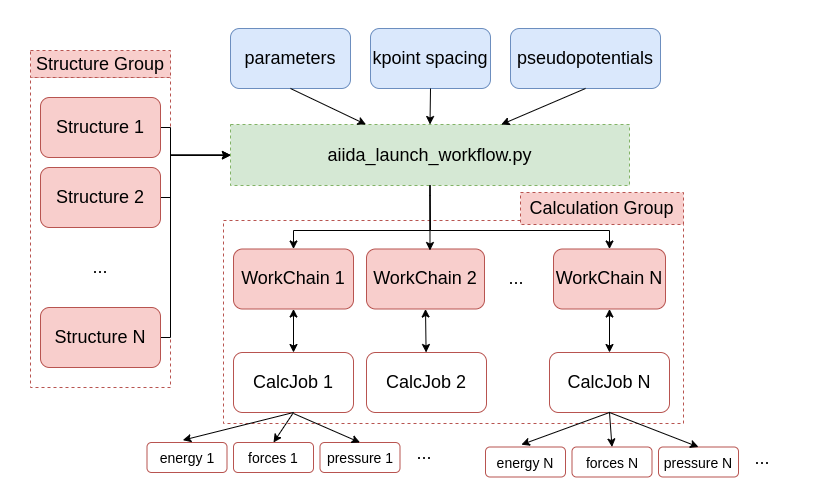
\includegraphics[width=1.0\textwidth,center]{figures/recalculateDBschematic.png}%
\caption{Schematic of AiiDA usage.  Structures are stored in the database in a \lstinline{Structure Group}; jobs are launched with the \lstinline{aiida_launch_workflow.py} wrapper script; each \lstinline{WorkChain} object manages a \lstinline{CalcJob} where common events, e.g., job submission, continuation of jobs past cluster time outs are handled automatically; outputs such as computed energies, forces, pressures and atomic structures are stored automatically in a database, organized in \lstinline{Calculation Groups} with typically one
for each \lstinline{Structure Group} of interest.
}
\label{fig:aiida_methods}
\end{figure}

\subsection{NNP selection and Evaluation of Errors} \label{sct:nnp_select_and_eval}

In this work, we generated neural network potentials (NNPs) using the methodology developed by Behler and Parrinello\cite{Behler2007} as implemented in the open source code n2p2 \cite{Singraber2019ParallelPotentials}.  Here we sketch the essentials of the method and refer the reader to the excellent tutorial review of Behler for further details \cite{Behler2015}. 

An NNP predicts the energy of an entire structure by summing energies of each atom within the structure as 
\begin{equation}
E^{structure} = \sum_i E^{atom}_i
\end{equation}
Each atomically-local energy, $E^{atom}_i$, is computed using a nested hierarchical function of weighted layers across a neural network.
We use a neural network architecture with two hidden layers and 24 nodes per layer.  We did not rigorously investigate other network architecture, and other configurations would likely work as well.  The functional form for the atomic energy is given explicitly as
\begin{equation}
E^{atom}_i = f_3 ( b^3_1+\sum^{24}_{k=1}a^{2,3}_{k,1}\cdot f^2_k(b^2_k+\sum^{24}_{j=1}a^{1,2}_{j,k}\cdot f^1_j ( b^1_j + \sum^{64}_{i=1} a^{0,1}_{i,j}\cdot G_i  ))) 
\end{equation}
Where $a^{q,p}_{z,w}$ is the weighting from node $z$ on layer $q$ to node $z$ on layer $w$, similarly $b^q_z$ is
the bias of node $z$ on layer $q$. $f_q$ is an activation function; here we use the softplus function 
$\ln (1 + \mathrm{e}^x)$ for $f_1$ with $f_2$ and $f_3$ the identity functions.

The $G_i$ are functions used to characterize a local atomic environment, and are generally referred to as the Descriptors. In the B-P NNP framework,
they are called symmetry functions.  We use radial and angular symmetry functions defined as
\begin{equation}
G^{radial}_i = \sum^{N_{atom}}_{j=1}e^{-\eta(R_{ij}-R_{s})^2}\cdot f_c(R_{ij})
\end{equation}
\begin{equation}
G^{angular}_i = 2^{1-\zeta}\sum_{j\neq i}\sum_{k\neq i,j}[ (1+\lambda\cdot cos\theta_{ijk})^\zeta \cdot e^{-\eta(R^2_{ij}+R^2_{ik}+R^2_{jk})}\cdot f_c(R_{ij}) \cdot f_c(R_{jk}) \cdot f_c(R_{jk}) ]
\end{equation}

Where $\eta$, $\zeta$ and $\lambda$ are pre-defined, or hyper-, parameters for a given symmetry function, $R_ij$ is the distance between atoms $i$ and $j$, and $f_c(r) = tanh^3(1-r/r_c)$ is a cut-off function where $r_c$ is a cutoff parameter for each symmetry function.
From among the above general class of symmetry functions, we select a subset based on the structures in our training dataset using the CURSEL method of Imbalzano et al. \cite{Imbalzano2018}.
First, we generate a dense grid hyperparameters to create a total of 1192 unique radial and angular symmetry functions.
We then performed a CUR decomposition on all 4857 structures and selected the 32 most-descriptive Al-centered symmetry functions and the 32 most descriptive Cu-centered symmetry functions for a total of 64 symmetry functions.
We found that 32 symmetry functions per atom type resulted in a good balance between accuracy and computational cost.The resulting list of symmetry functions is shown in Appendix \ref{apd_sct:symmfunc_hyperparam}.

Training of the NNP potential, i.e. determination of the weights and biases to best-match the DFT reference data, was accomplished with the n2p2 library\cite{Singraber2019ParallelPotentials}\cite{Singraber2019Library-BasedPotentials}.
We selected at random 90\% of the structures for training and the remainder for testing.
NNP weights were updated during the training using a fading memory Kalman filter.
The training is based on minimizing an objective, or loss, function.
We trained a loss function $\Gamma^{loss}$ on the total energy of the $i^{th}$ structure in the training set, $E_i$, as well as the $j^{th}$ force for that structure $F_{i,j}$:

%ADD IN THE DESCRIPTION HERE
\begin{equation}
\Gamma^{loss} = \frac{1}{N^{struct}} \sum^{N^{struct}}_{i=1}((E^{NNP}_i-E^{DFT}_i)^2+\frac{\beta}{3N^{atom}_i}\sum^{3N^{atom}_{i}}_{j=1}(F^{NNP}_{i,j}-F^{DFT}_{i,j})^2)
\end{equation}

where the sums are performed over all training structures $N^{struct}$ at each iteration of training.
Note that for each structure there is only one energy, $E_i$, but $3N^{atom}_i$ forces, i.e., 3 forces (X,Y,Z) for each atom.
$\beta$ controls the relative influence of forces on the loss function, in this study $\beta = 8$($\AA^2$).
We used 2.1\% of forces during each training epoch, (the n2p2 default is 2.3\%), increasing the ratio beyond this number resulted in prohibitive computational cost.
Note that this formulation tends to be biased towards larger structures since each atom independently contributes to the error. 
We use a standard 150 epochs (iterations) of training per NNP after which we found there to be only minimal gains in accuracy.  LAMMPS\cite{Plimpton1995} was used to compute the energies and forces of all structures using the evolving NNP during training via the n2p2 interface. 

Here, we generated 40 NNPs that differ in the specific 90\% training structures and the initial random weights and biases.  The initial training structure dominates the final NNP.  Note that these 40 NNP are thus not independent potentials.  However, they represent the range of potentials that are achieved using this NNP structure, symmetry functions, and set of training structures.  Their predictions for various material properties thus represent the range of properties associated with these NNP details.  The set of 40 NNPs can be used as a committee model to assess whether a particular new structure outside the overall training dataset may or may not be accurately represented.  To present one specific set of results for many different properties, we select one NNP from among the 40 NNPs, labelled NNP11, that has the lowest error for $C_{44}$ in Al. This choice is motivated by the importance and relative difficulty of modeling $C_{44}$ accurately.  In results below, all error bars center on the average of all 40 trained NNPs and indicate +/- one standard deviation.  The NNP11 may fall near the average or outside the error bars; it is just one particular NNP.  This also highlights the care necessary in considering the average and standard deviation across the 40 NNPs: there may not be any single NNP that is within one standard deviation of the average for all properties considered.  Lastly, we reiterate that the standard deviation does not indicate statistically independent results since all NNPs are trained on very similar sets of structures.

\section{Results: NNP versus Training and Test Data}

\subsection{Overall NNP accuracy} \label{sct:test_and_train_errors}
Here we look at the root mean square error (RMSE) for structures in the testing and training sets for both energies and forces separately,

\begin{equation}
    RMSE(E) = (\frac{1}{N^{struct}}\sum_i^{N^{struct}} (E^{DFT}_i - E^{NNP}_i)^2)^\frac{1}{2}
\end{equation}
\begin{equation}
        RMSE(F) = (\frac{1}{N^{struct}}\sum_i^{N^{struct}}\sum_j^{3N^{atom}_i}\frac{1}{3N^{atom}_i} (F^{DFT}_{i,j} - F^{NNP}_{i,j})^2)^\frac{1}{2}
\end{equation}
Over all 40 NNPs there is an average RMSE for the energy of 2.49 meV/Atom for testing and 69.15 meV/atom for training, while the testing and training RMSE for the forces are 23.9 meV/$\AA$ and 35.93 meV/$\AA$, respectively.  These would appear to be unacceptably large testing errors, indicating poor potential quality.  In fact, most of the NNPs show only a modest difference, with 21 out of the 40 potentials having a testing RMSE for energy of less than 5 meV/atom.  The major contributor to the large error in the RMSE values for the remaining potentials is due to a single outlier structure under very high compression.  Examining NNP11 as an example, the  RMSE for energy is 2.58 meV/atom for the training set but 26.51 meV/atom for the testing set, but the histogram of errors shown in Figure \ref{fig:rsme_histogram} (a) reveals the single outlier, which is FCC Al at lattice constant $a/a_0 =0.81$.   The testing RMSE for NNP11 without this outlier structure would fall to a very acceptable value of only 3.46 meV/atom. The forces follow a nearly uniform error distribution, and does not have an outlier like in the energies, as can be seen in Figure \ref{fig:rmse_histogram} (b).  
For all other NNPs with high test/train error ratios, the cause was found to be outlier structures with $a/a_0 ~= 0.8$. 

\begin{figure}[H]%
\centering%
\subfloat[]{{
 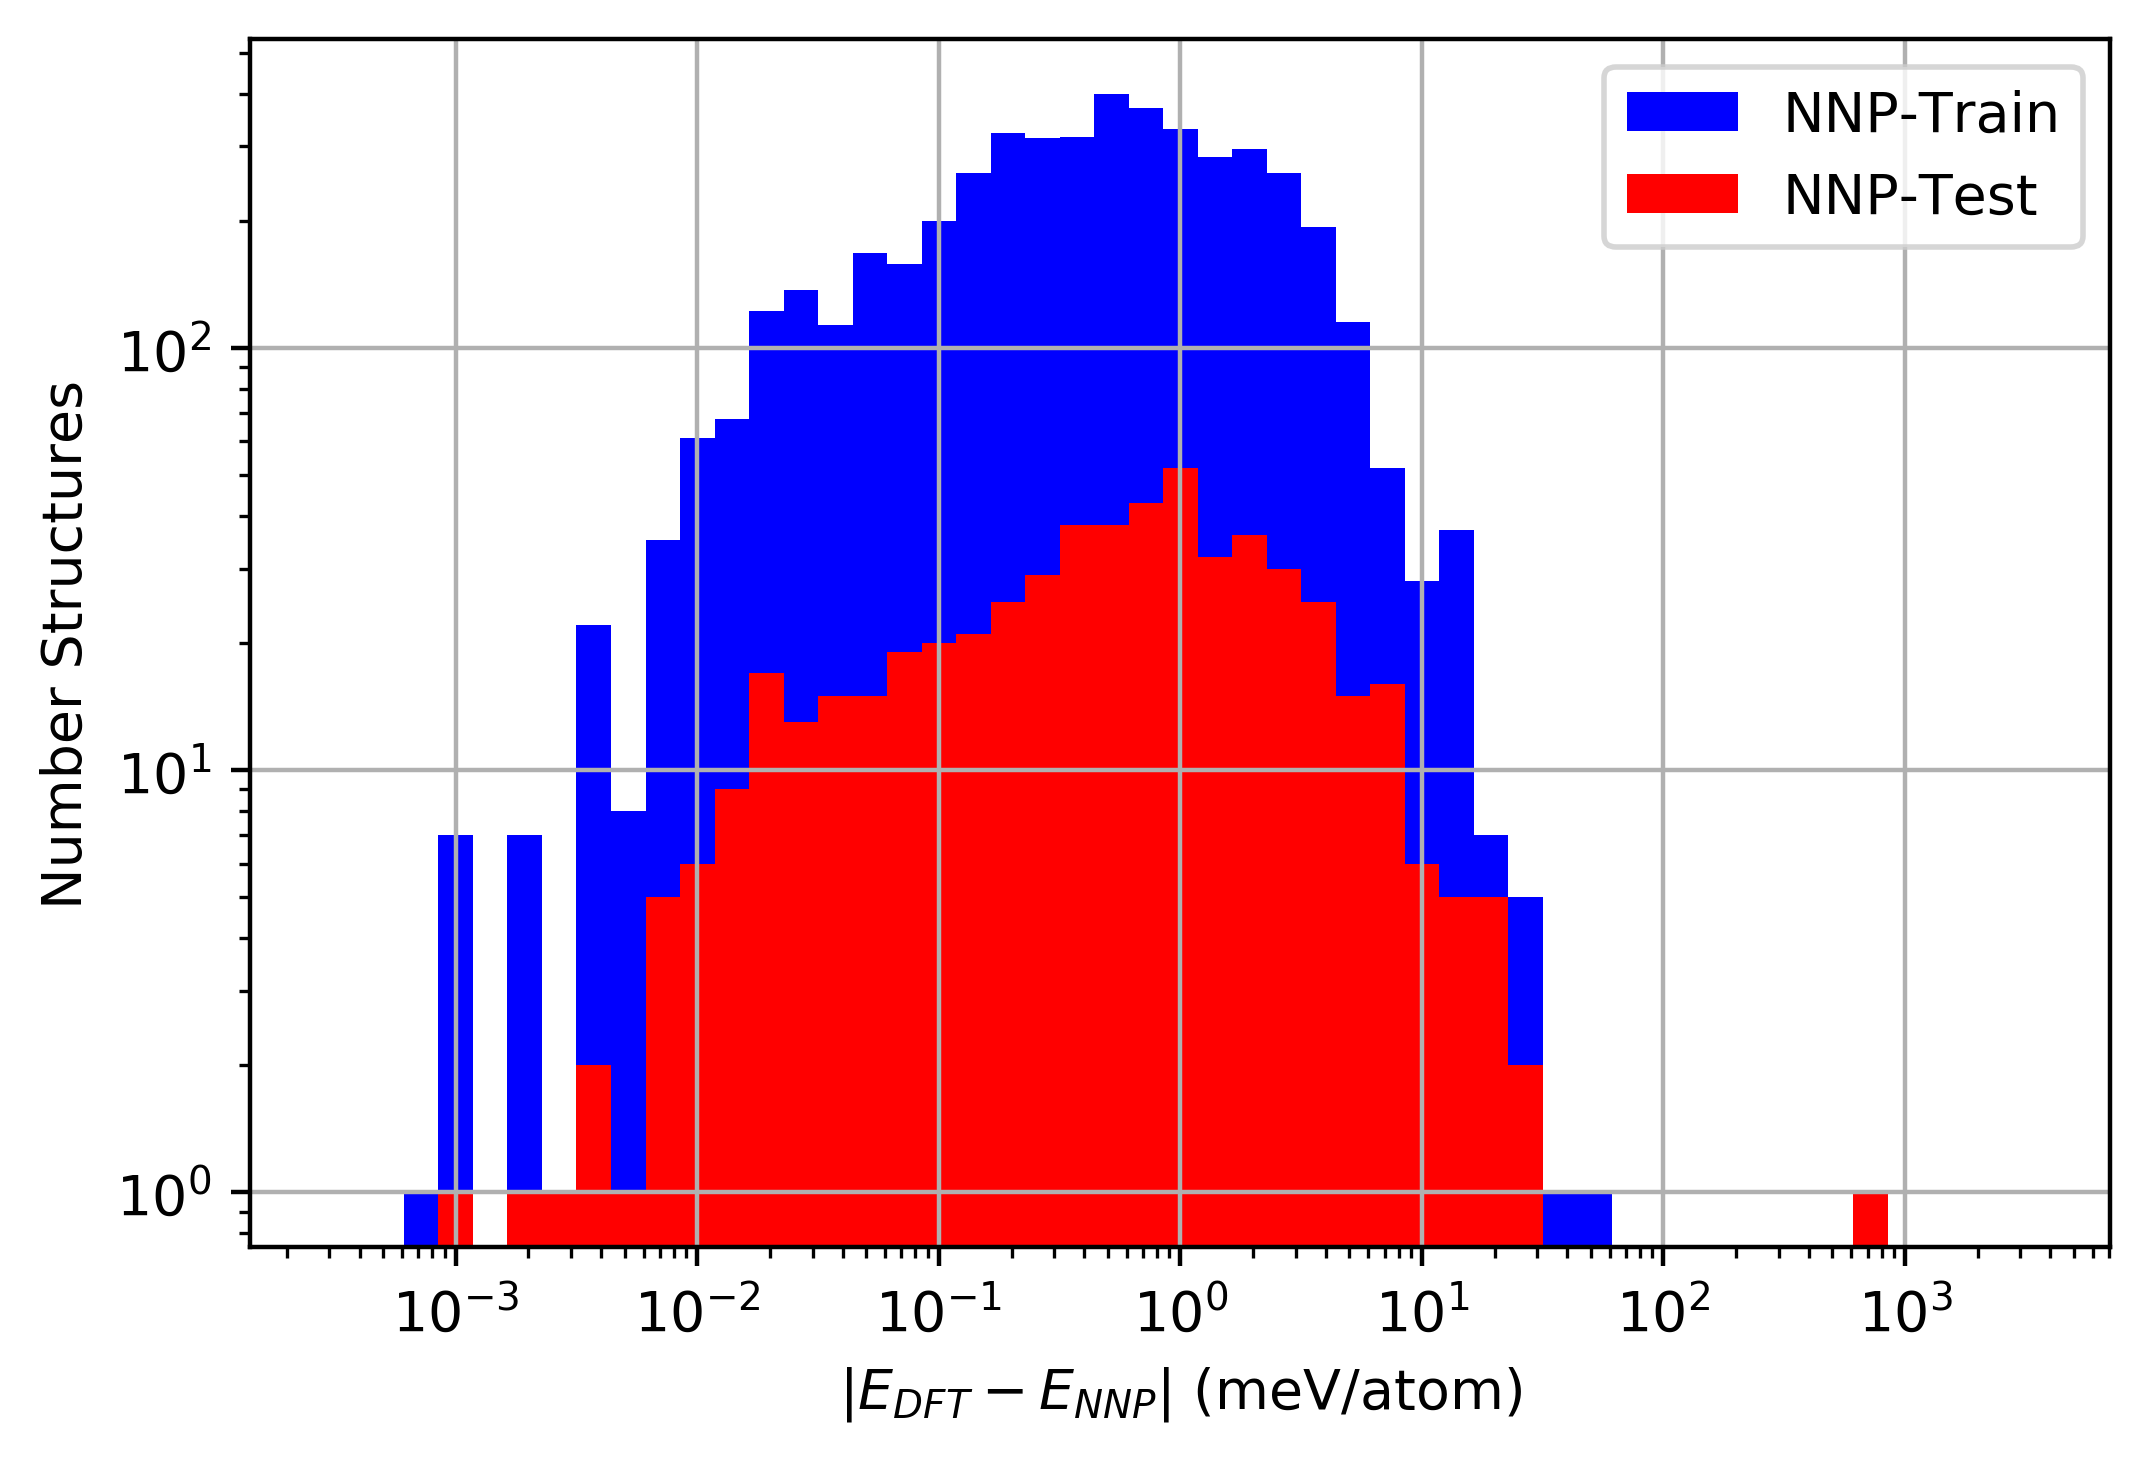
\includegraphics[width=0.50\textwidth]{figures/plot_nnperrors_histogram.png}
 }}%
\subfloat[]{{
 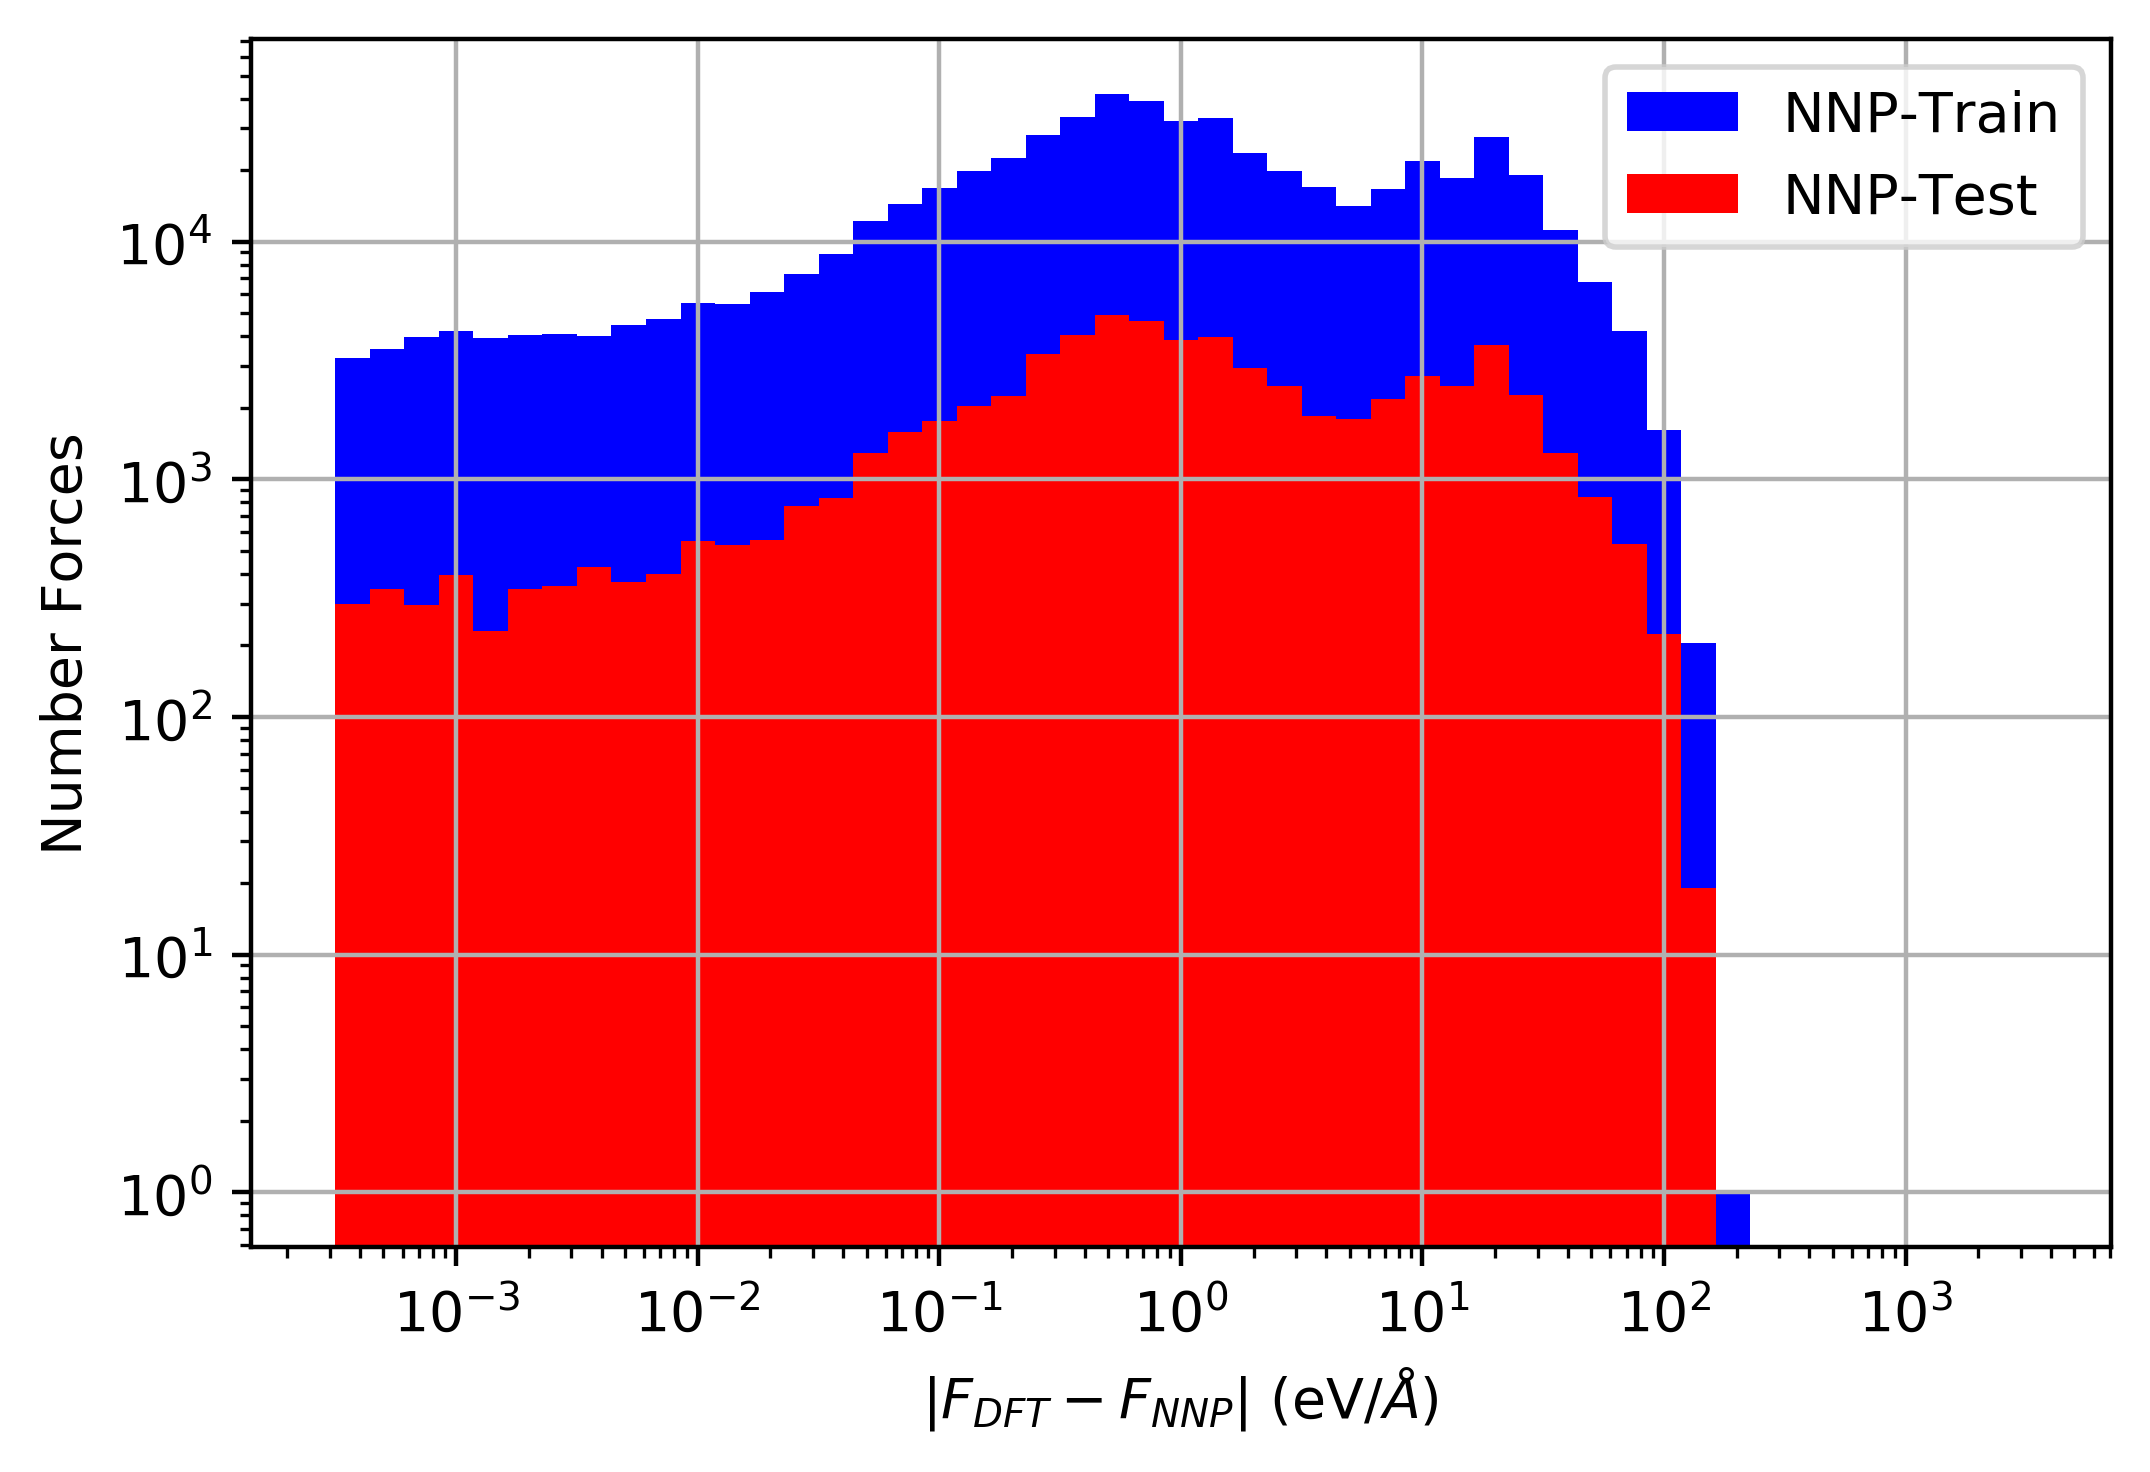
\includegraphics[width=0.50\textwidth]{figures/plot_nnperrors_forces_histogram.png}
 }}%
\caption{Histogram of errors for the (a) energy and  (b) forces for both training and testing for NNP11}
\label{fig:rsme_histogram}
\end{figure}

The predictions of ML potentials at high compression outside the domain of training is commonly highlighted as a failure of NNPs.
In fact, such behavior is easily prevented by the addition of a strongly repulsive potential for small atomic spacings, and such an ad-hoc potential is part of standard EAM/MEAM potentials to handle exactly this behavior.
Of equal importance is that there are few, if any, metallurgical problems where such a high compression and high energy structure could be accessed.  Here, the NNPs have high error when the training set does not include the structures with $\frac{a}{a_0} ~= 0.8$, as can be seen in Appendix \ref{apd_sct:eos_data}. Putting aside this unusual structure - which can be captured if it is included in the training set - all 40 NNPs perform very well overall.


\subsection{Bulk Properties} \label{sct:bulk_properties}

Figure \ref{fig:matparam_purestats} shows the fractional deviation with respect to the DFT reference value for a number of fundamental properties in pure Al and Cu as predicted by the NNP and ADP.  For the lattice and elastic constants and surface energies, to which the ADP is directly fit, the NNP shows no advantage relative to ADP. The NNP only improves over ADP in the predicted stable stacking fault energies in Al.
The NNP shows substantially different values for $C_{44}$ of Al as compared to DFT, systematically too large by ~20\%.  Such a deviation is not unusual for NNPs, and prior work has found errors of a similar magnitude for elastic constants \cite{Zuo2020APotentials}.
Elastic constants are derived from the second derivative of the energy around the minimum energy, and so are presumably challenging to model accurately
when training is performed primarily on energies and on a training set with a very wide distribution of energies relative to the bulk perfect crystal.  
We note that the error is not in the DFT because the DFT parameters have been carefully converged with respect to $C_{44}$.  Otherwise, for the basic properties to which EAM/MEAM-type potentials are fit, the NNP performs roughly as well as the ADP.

\begin{figure}[H]%
\centering%
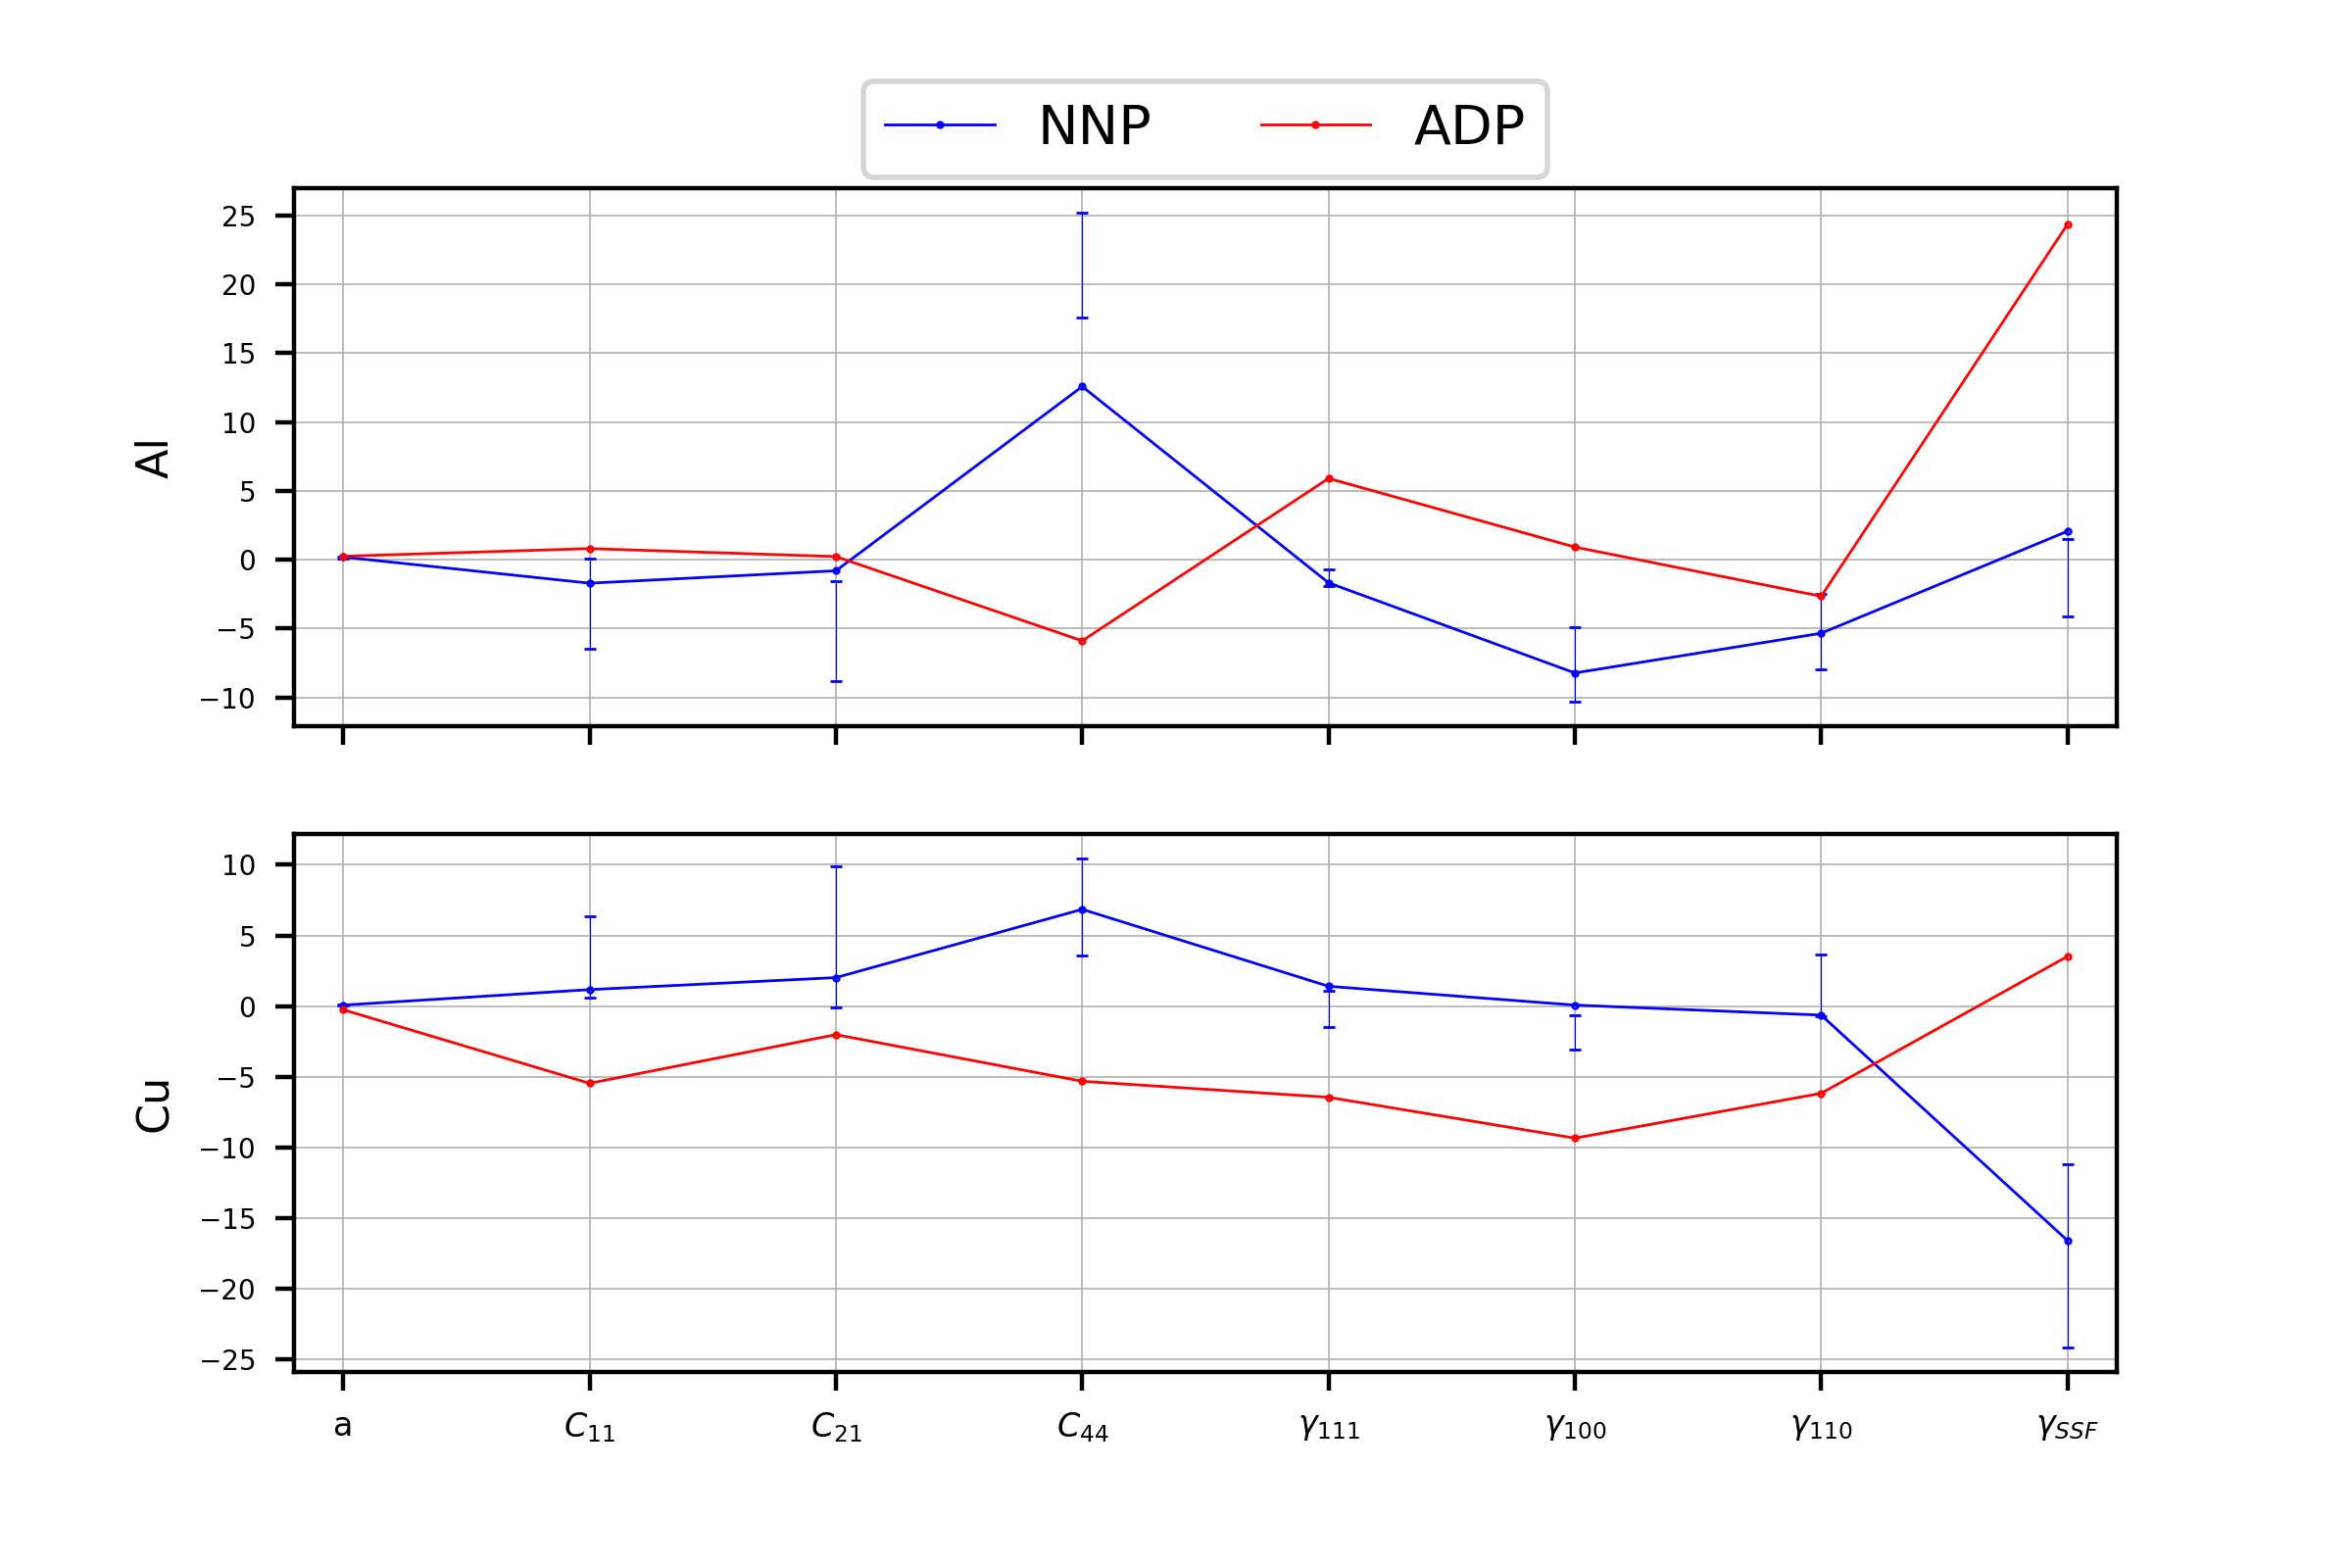
\includegraphics[width=1\textwidth,center]{./figures/matparam_purestats.png}%
\caption{Deviation of NNP and ADP properties from DFT reference values (\%) for lattice constants, elastic constants, surface energies, and stable and unstable stacking fault energies of FCC Al and Cu.  Dashed blue lines and error bars: mean and standard deviation across 40 NNPs; dark blue line: NNP11; red lines: ADP.  
All structures from which these properties are derived are included in the training set. }%
\label{fig:matparam_purestats}
\end{figure}

Figure \ref{fig:matparam_stats1} shows the formation energies, atomic volumes, and elastic constants for all Al-Cu intermetallic structures within the OQMD database as computed via DFT, the NNPs (mean, standard deviation, and the specific NNP11), and the ADP.
The formation energy $\Delta E^{structure}_f$ of each structure is computed relative to bulk FCC Al and dilute solid-solution Cu in the Al matrix as
\begin{equation} \label{eqn:formE_structure}
\Delta E^{structure}_f = E^{structure}_N - nE^{ref}_{Al}-(N-n)E^{ref}_{Cu}
\end{equation}
\begin{equation} \label{eqn:formRef_Al}
E^{ref}_{Al} = E^{FCC}_{Al}
\end{equation}
\begin{equation} \label{eqn:formRef_Cu}
E^{ref}_{Cu} = E^{1sol}_{255Al,1Cu} - 255E^{FCC}_{Al}
\end{equation}
Where $N$ and $n$ are the total number of atoms and number of Al atoms, respectively, in a given structure.  The formation energies are generally very well predicted by the NNPs, with most errors within a few meV/atom.  In contrast, the ADP often highly overestimates or underestimates the formation energy;
in a few cases, ADP reverses the sign relative to pure Al.  The B2 structure poses a challenge to both ADP and most NNPs.  The ADP predicts the B2 phase to be extremely stable - more stable than any other structure - while the NNP predictions have the highest error among all structures considered.  Some NNPs have, however, good predictions for the B2 phase and the NNPs largely preserve the overall order of stability among the many different phases.  For structures with high formation energy, both the NNP and ADP show inaccuracies, often not relaxing to the same structure as DFT or having substantial errors, especially the ADP.  The ADP regularly underestimates the atomic volume, even for the critical $\theta$ and $\theta'$ structures.  Since strain energies due to lattice mismatch can contribute to in-situ precipitate formation energies, these large deviations in volume can lead to substantial erroneous effects.  
For elastic constants, neither the ADP nor the NNPs are extremely accurate but overall the NNPs are superior to the ADP, especially for the important low-energy structures. 

\begin{figure}[H]%
\centering%
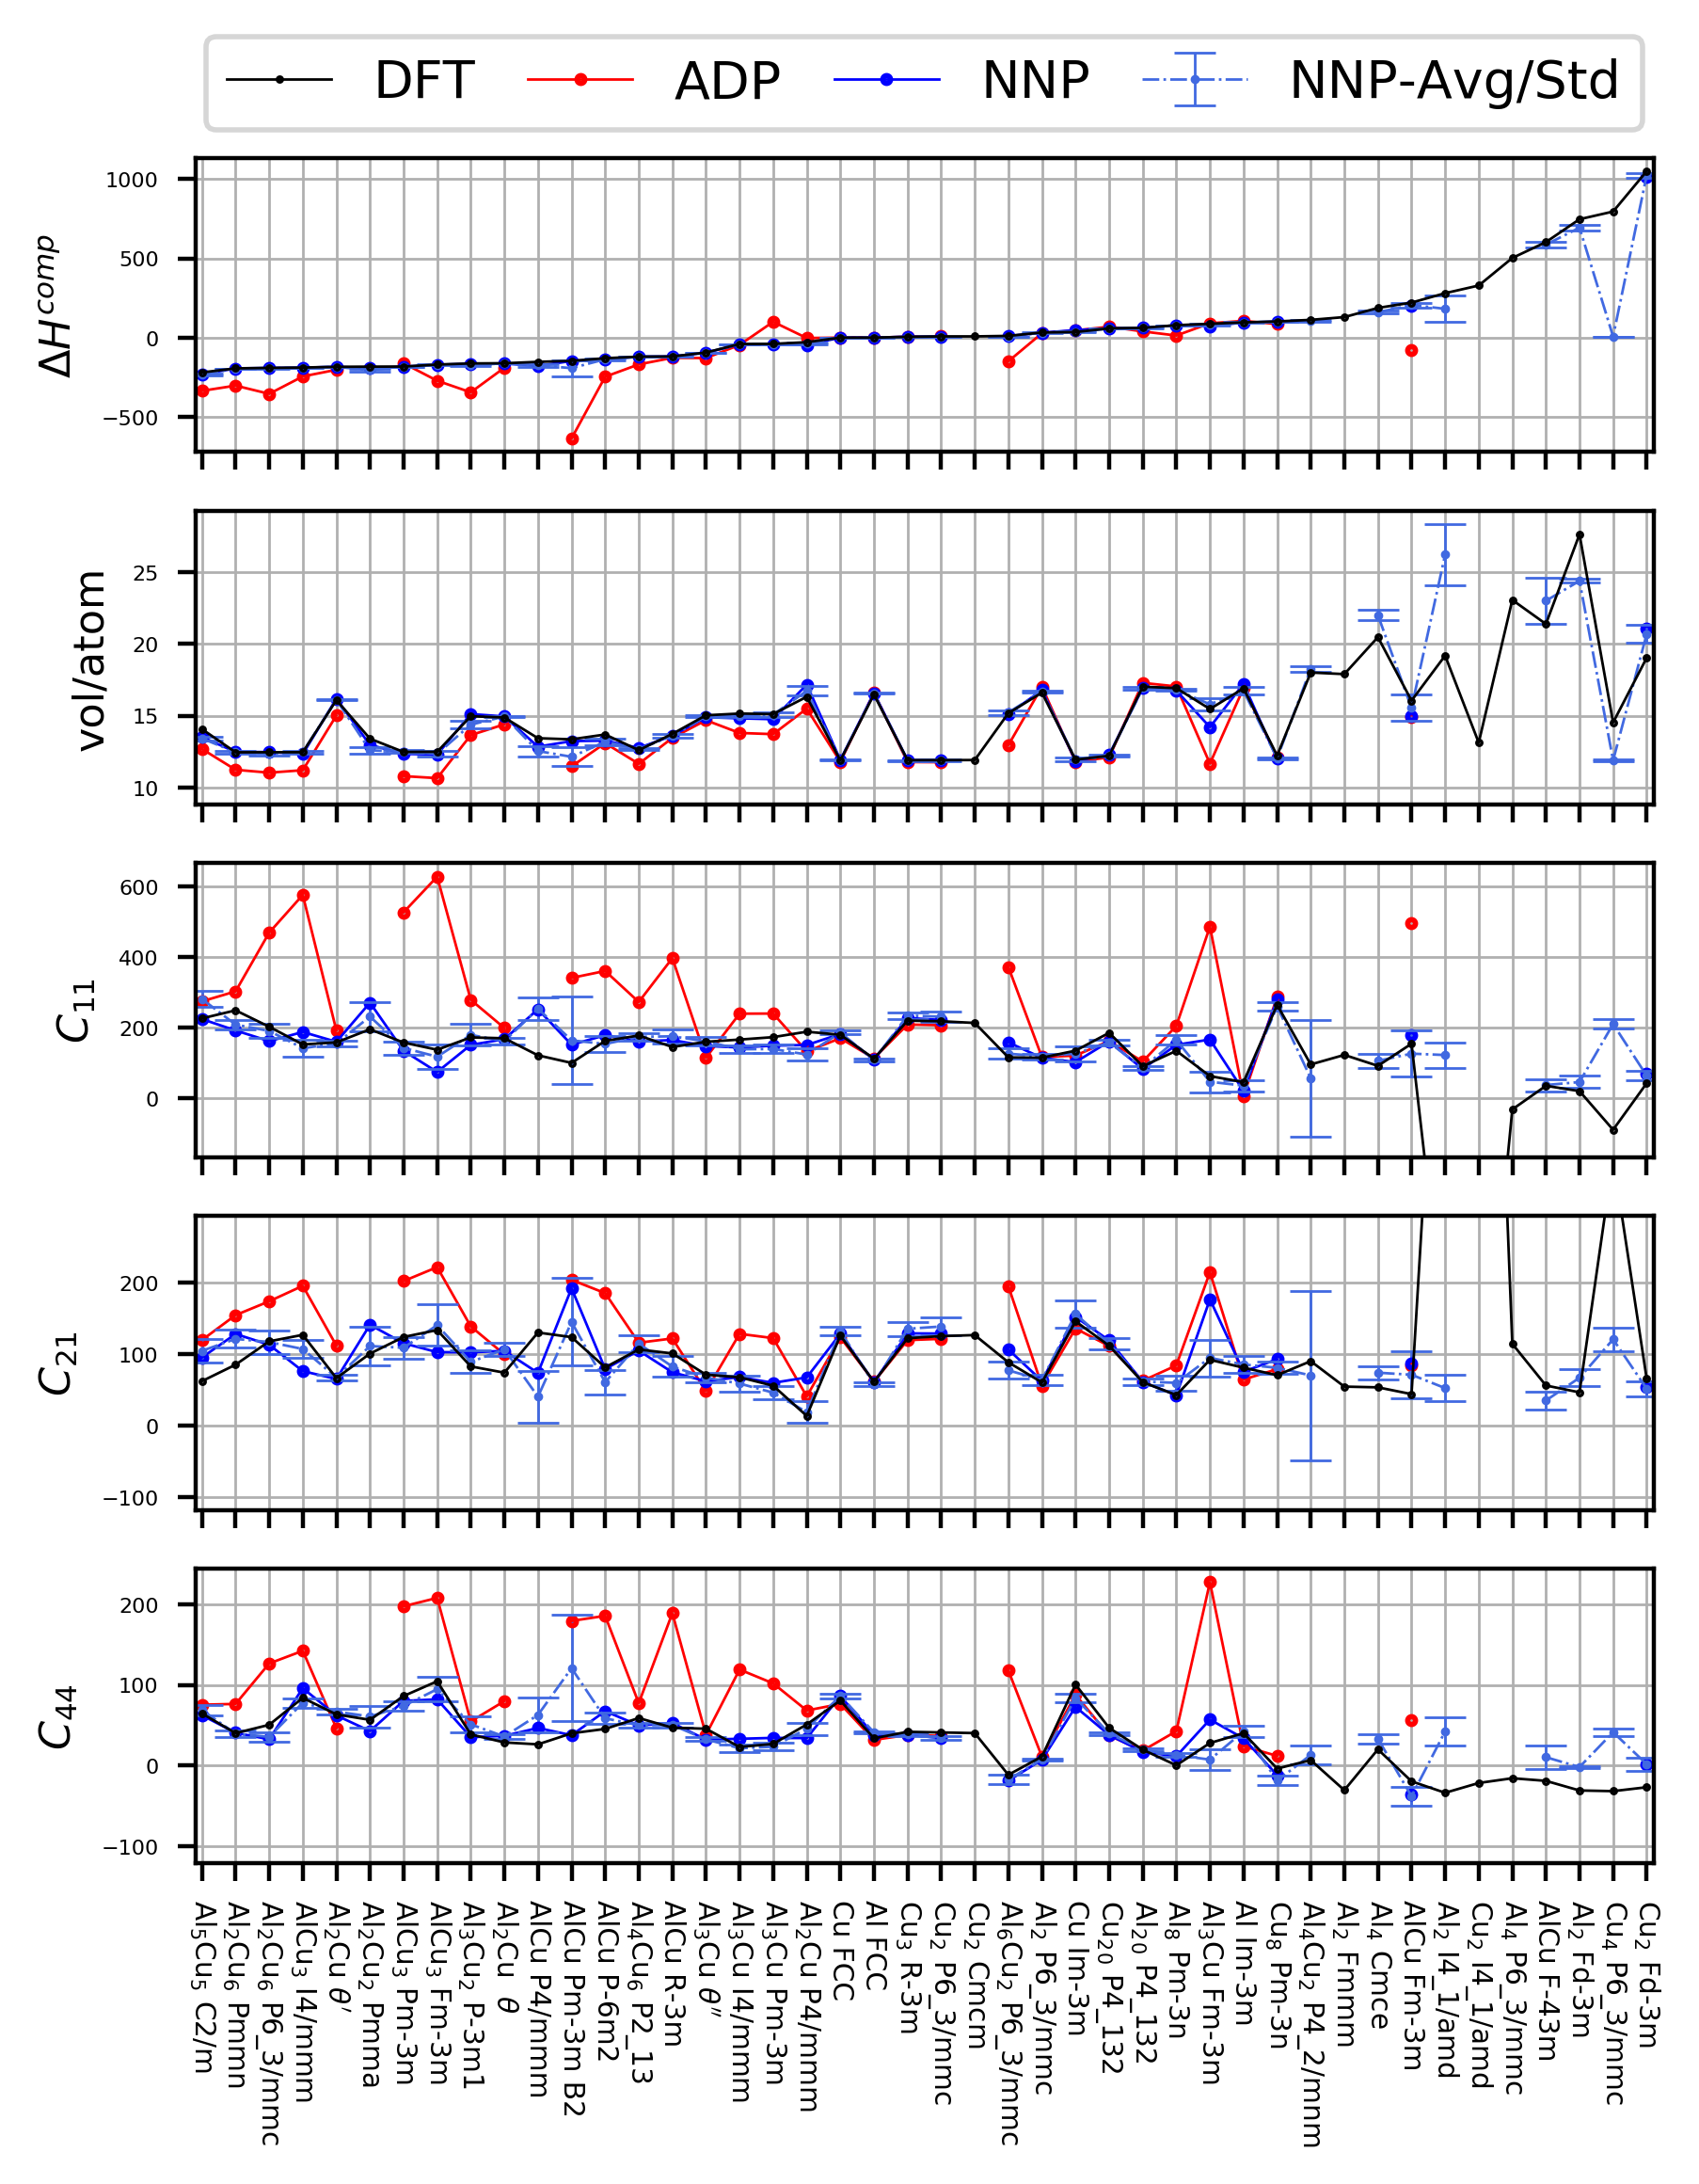
\includegraphics[width=1\textwidth,center]{figures/matparam_stats1.png}%
\caption{Formation energy, atomic volume, and elastic constants C$_{11}$, C$_{21}$ and C$_{44}$ as predicted by DFT, the NNPs, and the ADP, versus structure, for all Al-Cu structures in the OQMD database.  All structures from which these properties are derived are included in the training set.}
\label{fig:matparam_stats1}
\end{figure}

\subsection{Solutes} \label{sct:solute_results}

The binary formation energies for Cu, Al, and Vacancy in Al or Cu matrix are computed as
\begin{equation}
\Delta E^{bind}_f = E^{2sol}_{N-2,X,Y}-E^{1sol}_{N-1,X}-E^{1sol}_{N-1,Y}+E^{pure}_N
\end{equation}
Where $\Delta E^{bind}_f$ is the binding energy for the solute pair, with a negative energy indicating attraction.
$E^{2sol}_{N-2,X,Y}$, $E^{1sol}_{X}$, $E^{1sol}_{Y}$, $E^{1sol}_{Y}$ are the energies for a solute pair, a single solute of species X, a single solute of species Y, and a system of pure bulk matrix respectively. 
Here N=256 for Al matrix and N=108 for Cu matrix. 
The DFT, NNP, and ADP results for these quantities in Al are shown in Figure \ref{fig:solsol_in_al} while those for the Cu matrix are shown in Appendix \ref{apd_sct:adn_solsol}.  The NNP predictions for pair binding energies are generally in good agreement with DFT, typically within 25 meV (kT at room temperature) across all NNPs, and notably better than the predictions of the ADP.  The NNP11 near-neighbor Cu-Vacancy and Vacancy-Vacancy binding energies do deviate from the DFT values by 20 meV, but the ADP predicts massive overbinding of Cu-Cu and Cu-Vacancy near-neighbor pairs and underbinding of Cu-Cu third and fourth neighbors.  While these ADP values collectively lead to reasonable formation energies for the $\theta$ and $\theta'$ structures (see Figure \ref{fig:matparam_stats1}), it is evident that such agreement is due to significant cancellations of errors among the different pair interactions.  These pair interactions would also have serious negative implications for kinetic studies of precipitation using the ADP.

\begin{figure}[H]%
\centering%
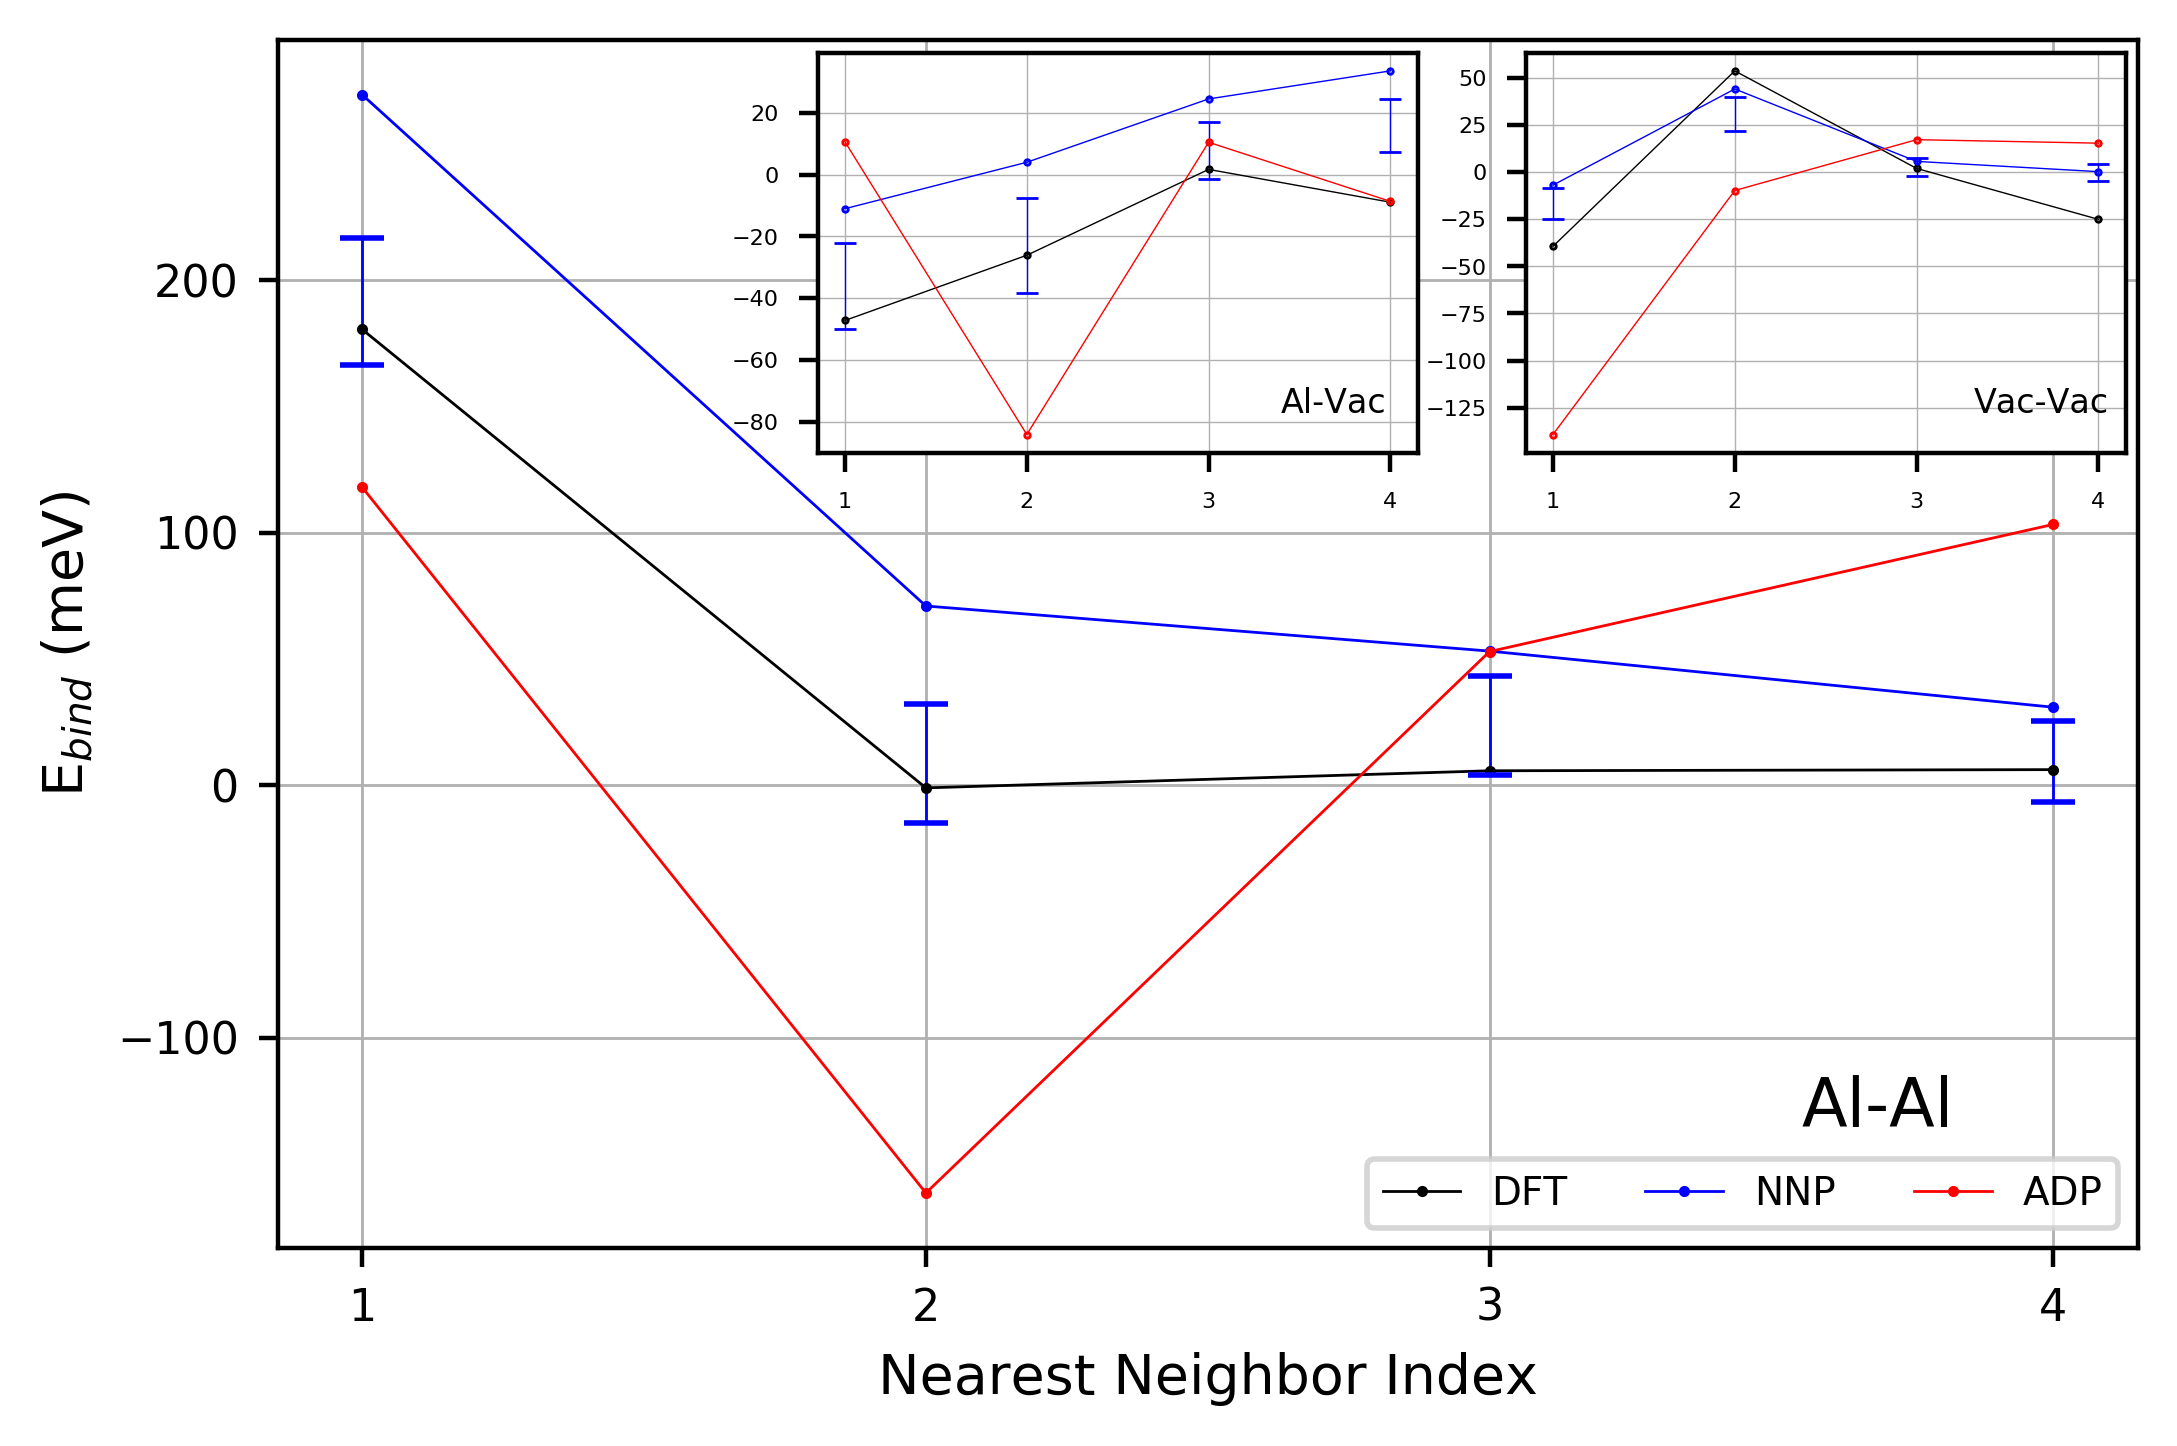
\includegraphics[width=1\textwidth,center]{./figures/solsol_in_al.png}%
\caption{Pair binding energies for Cu-Cu, Cu-Vac, and Vac-Vac pairs in an Al matrix as a function of near neighbor index. 
ADP predicts huge errors for Cu-Cu first-neighbor binding (-318 meV) 
while third and fourth neighbors are far too repulsive (108meV and 175meV, respectively). 
Relevant structures are included in the training set.
}%
\label{fig:solsol_in_al}
\end{figure}

Table \ref{table:solute_misfit_SF} shows the solute misfit volumes for Cu in Al and Al in Cu, as predicted by DFT, the NNPs, and the ADP.  The misfit volumes are computed from the relaxed total volumes of cells containing one solute when using the potentials.  When using DFT, we fix the cell size at the bulk elemental value, measure the induced pressure upon introduction of the solute, and compute the misfit volume using the pressure and metal bulk modulus.  The ADP is grossly incorrect for Cu in Al.  This is the origin of reported difficulties in measuring solid-solution strengthening of dilute Al-Cu alloys\cite{Singh2013AnAlloy}.   The ADP also predicts the incorrect sign for the volume of Al in Cu.  The NNPs show a range of values around the DFT value for Cu in Al, with NNP11 in reasonable agreement.  The NNPs for Al in Cu are slightly smaller than, but within the range of, the DFT, although NNP11 predicts a particularly small value.  Solute strengthening at T=0K scales as $(misfit volume)^{4/3}$, and hence the deviation for the NNP11 is not negligible for accurate prediction of solute strengthening but other NNPs could yield suitable values for misfit volume but offset by larger errors in the elastic constants.

Table \ref{table:solute_misfit_SF} also shows the solute/stacking fault interaction energies for Cu in Al and Al in Cu, as predicted by DFT, the NNPs, and the ADP.
This interaction energy is computed from various system energies as
\begin{equation}
\Delta E^{Sol-SF}_{f,(N-1,X)} = E^{Sol-SF}_{N-1,X} - E^{SF}_{N} - (E^{1sol}_{N-1,X}-E^{Pure}_{N})
\end{equation}
Where $E^{Sol-SF}_{N-1,1}$ is the energy of a system containing the stacking fault and a single solute,
$E^{SF}_{N}$ is the energy of the system with the stacking fault alone. 
For Cu in Al, the NNPs are in good agreement with DFT while the ADP value is far too large.  In contrast, for Al in Cu, the ADP value
is in reasonable agreement with DFT while the NNP values are too small and around zero.  This energy can enter into solute strengthening\cite{Leyson2010} and is crucial for dynamic strain aging (DSA) \cite{Curtin2006}.  With Cu-15at\%Al a classic alloy for DSA, the ADP appears better than the NNP but actually remains unsuitable due to the error in the misfit volume.

\begin{table}[H]
\begin{tabular}{l|cccc}%
\hline%
&DFT&ADP&NNP11& NNP-\emph{Avg / StdDev}\\%
\hline%
Misfit Vol Cu in Al ($\AA^3$)&{-}5.770&{-}16.958&{-}4.380&\emph{-7.095 / 1.076}\\%
Misfit Vol Al in Cu ($\AA^3$)&2.421&{-}1.259&0.109&\emph{1.334 / 0.857}\\%
SolSF Cu in Al (eV)&0.052&0.108&0.042&\emph{0.062 / 0.030}\\%
SolSF Al in Cu (eV)&{-}0.049&{-}0.034&{-}0.006&\emph{0.002 / 0.031}\\%
\hline%
\end{tabular}%
\caption{Misfit Volumes and solute-stacking fault interactions for DFT, ADP and NNP.}
\label{table:solute_misfit_SF}
\end{table}

\subsection{Interface and Generalized Stacking Fault Energies} \label{sct:interfaces}

The interface energy between a precipitate and a matrix is an important component of the thermodynamics of nucleation and growth of nanoscale precipitates.  In addition, the interaction of a matrix dislocation with a precipitate is first dominated by the dislocation/interface interactions.  It is thus important that any potential provide an accurate description of the precipitate/matrix interfaces.  This is challenging due to the absence of information about the interface structure, but machine learning of the energies of approximate structures is valuable for providing some guidance to potentials for modeling of fully-relaxed interfaces.  Interface energies are almost never considered in the fitting of EAM-type potentials, leading to significant quantitative issues when interface-dominated phenomena are studied. 

The interface energy is computed as in \cite{Vaithyanathan2004MultiscaleAlloys}, and is briefly summarized here.
The formation energy for an interface with N atoms of which X are of the matrix and Y are of the precipitate,
$\Delta E^{interface}_{f, (X,Y)} = E^{interface}_{X,Y}-XE^{Matrix}_{bulk}-YE^{Precip}_{bulk}$,
is related to the number of atoms as
\begin{equation}
\Delta E^{interface}_{f,(X,Y)} = \delta E^{strain}_{X,Y} + \frac{2A\gamma^{interface}}{N}
\end{equation}
Where $\Delta E^{interface}_f$ is the interface formation energy, $\delta E_{strain}$ is the strain energy, $A$ the surface area,
$\gamma^{int}$ the interface energy, and $N=X+Y$ the total number of atoms in interface.
During relaxation, atoms are free to move, but the overall cell size and shape are held fixed.
The interface surface energy $\gamma^{interface}$ is then the slope of $\Delta E^{interface}_f$ versus $\frac{1}{N}$ and divided by $2A$.

Figure \ref{fig:interface_energies} shows the computed interface energies from DFT, the NNPs, and the ADP.
The ADP correctly predicts the general trends but makes several serious errors.
The coherent $\theta'$ interface energy is far too high while all the $\theta''$ interfaces are predicted to have negative energy.
The $\theta''$ interface is particularly challenging because it has such low interface energy; therefore, it is easy for a potential to predict a negative value.
In contrast, NNP11 shows good predictions versus DFT for all of these interfaces.  More details on the underlying data for these energies are given in Appendix \ref{apd_sct:add_interface} of the supplementary material.

\begin{figure}[H]%
\centering%
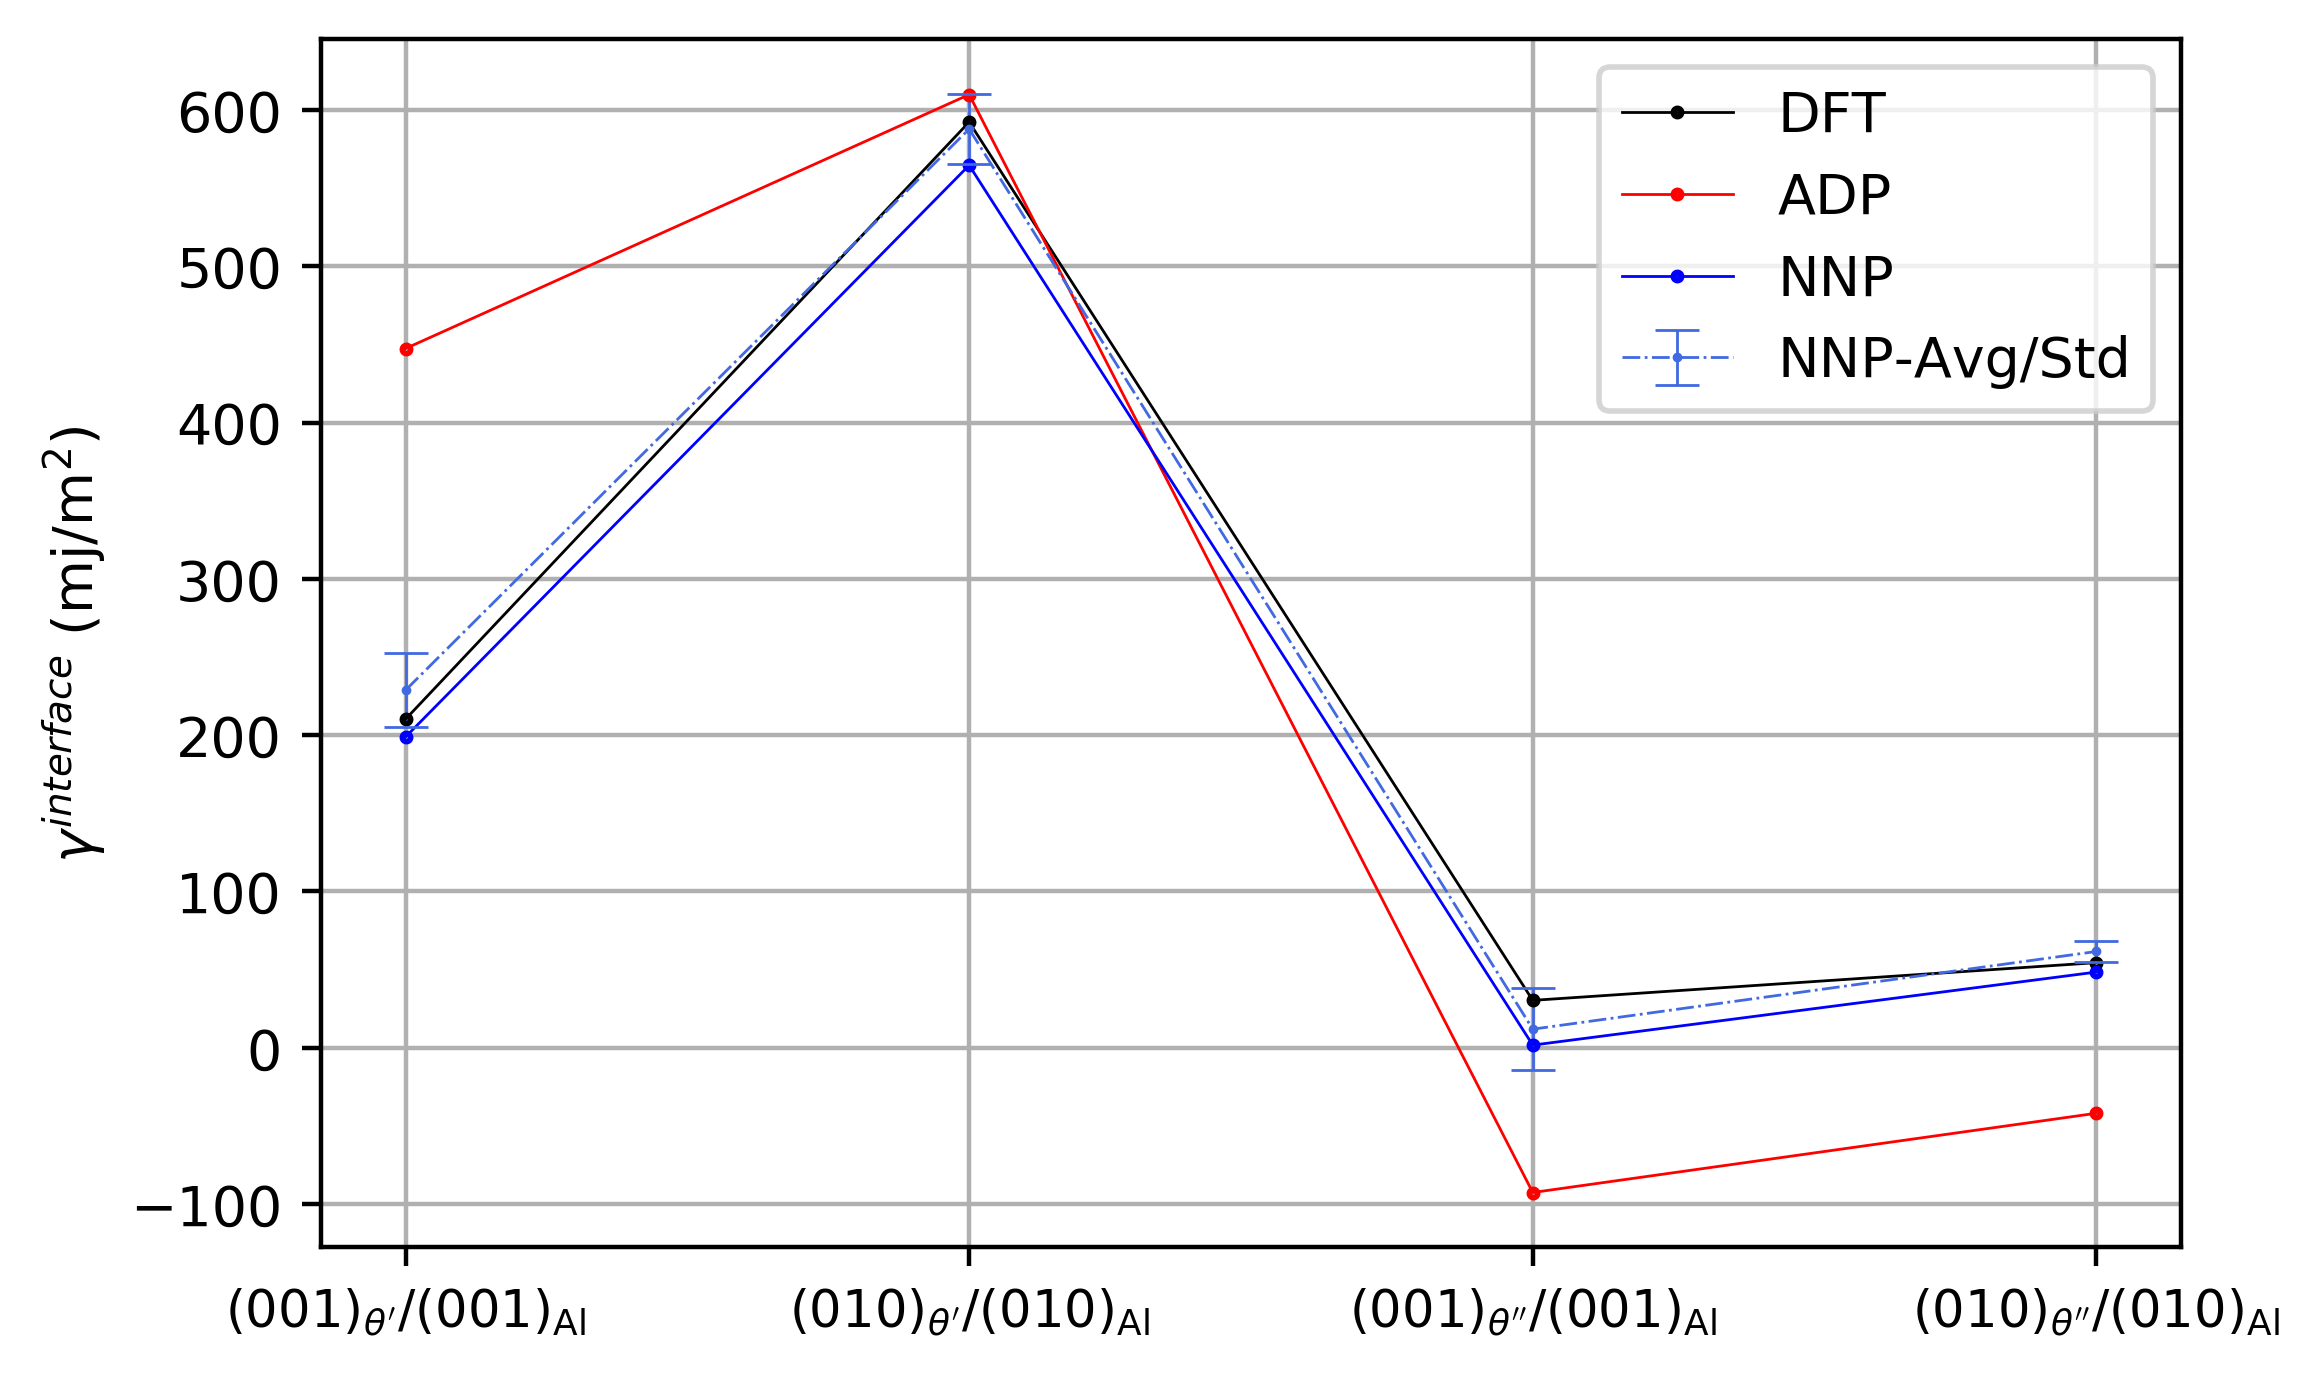
\includegraphics[width=1\textwidth,center]{./figures/interface_energies.png}%
\caption{Interface structure vs. interface energy for precipitate structures. 
These are the $\theta'$ coherent, $\theta'$ semi-coherent, $\theta''$ coherent and $\theta''$ semi-coherent
interfaces in order. Relevant structures are included in the training set. 
Figure \ref{fig:interface_structures} in the supplementary shows the atomic structure of these interfaces.
}%
\label{fig:interface_energies}
\end{figure}

The GSF energy surface (GSFE) determines the stable faults for the dissociation of dislocations, the core structure of such dissociated partial dislocations, and the energies related to shearing of the material.  For precipitates in Al, the GSFE for surfaces best-aligned with the (111) slip planes in Al determine the resistance of the precipitate to shearing and hence control the strength of the alloy.  It is thus important that the GSFE well-represent all phases that would be used to study dislocation motion and strengthening.  

The GSFE is computed using the methods detailed in \cite{Yin2017a}, which we briefly summarize here.
The smallest periodic cell vectors a1 and a2 for the desired slip surface are first identified, and a supercell created with a3 normal to the a1-a2 plane.  The  energy of the undeformed cell $E_{pristine}$ was computed.
For each vector $\vec{t}$ of the GSF, the periodic cell shape was deformed by shifting a3 by $\vec{t}$.  All atoms and the a3 cell vector were then allowed to relax in the 3-direction only to compute the energy $E^{GSF}_{\vec{R}}$.
The GSF energy at a displacement $\gamma_{GSF\vec{t}}$ was then calculated as 
\begin{equation}
\gamma^{GSF}_{\vec{t}} = (E^{GSF}_{\vec{t}} - E^{pristine})/A
\end{equation}
where $A$ is the area of the slip surface in the simulation cell.

Figure \ref{fig:GSF_Theta_0m11} shows the geometry and GSFE surface for the (0$\overline{1}$1) for the $\theta$ phase as computed by NNP11 and the ADP, and the energies at the local minima and maxima as computed by DFT, all the NNPs, and the ADP.  The NNPs all predict the extremal values in very good agreement with DFT.
In contrast, at the extremal points, the ADP deviates significantly from the DFT for the unstable points 4, 6, and 7, and remains quantitatively much worse than the NNP for the sites 2, 3, and 5.  The remainder of the GSFE surface is outside of the DFT training set.  The GSFE for the NNP11 is smooth while the ADP shows very sharp gradients that are not expected to be realistic.  The normal concern about ML potentials is that they may have sharp gradients and highly inaccurate energies in regions away from the training set, but the present results demonstrate that it is the traditional ADP potential that suffers from such issues.  The GSFE results for the NNP11 indicate that the NNPs can be used reliably for the study of $\theta$ precipitate shearing whereas the ADP cannot.

\begin{figure}[H]%
\centering%
\subfloat[]{{
 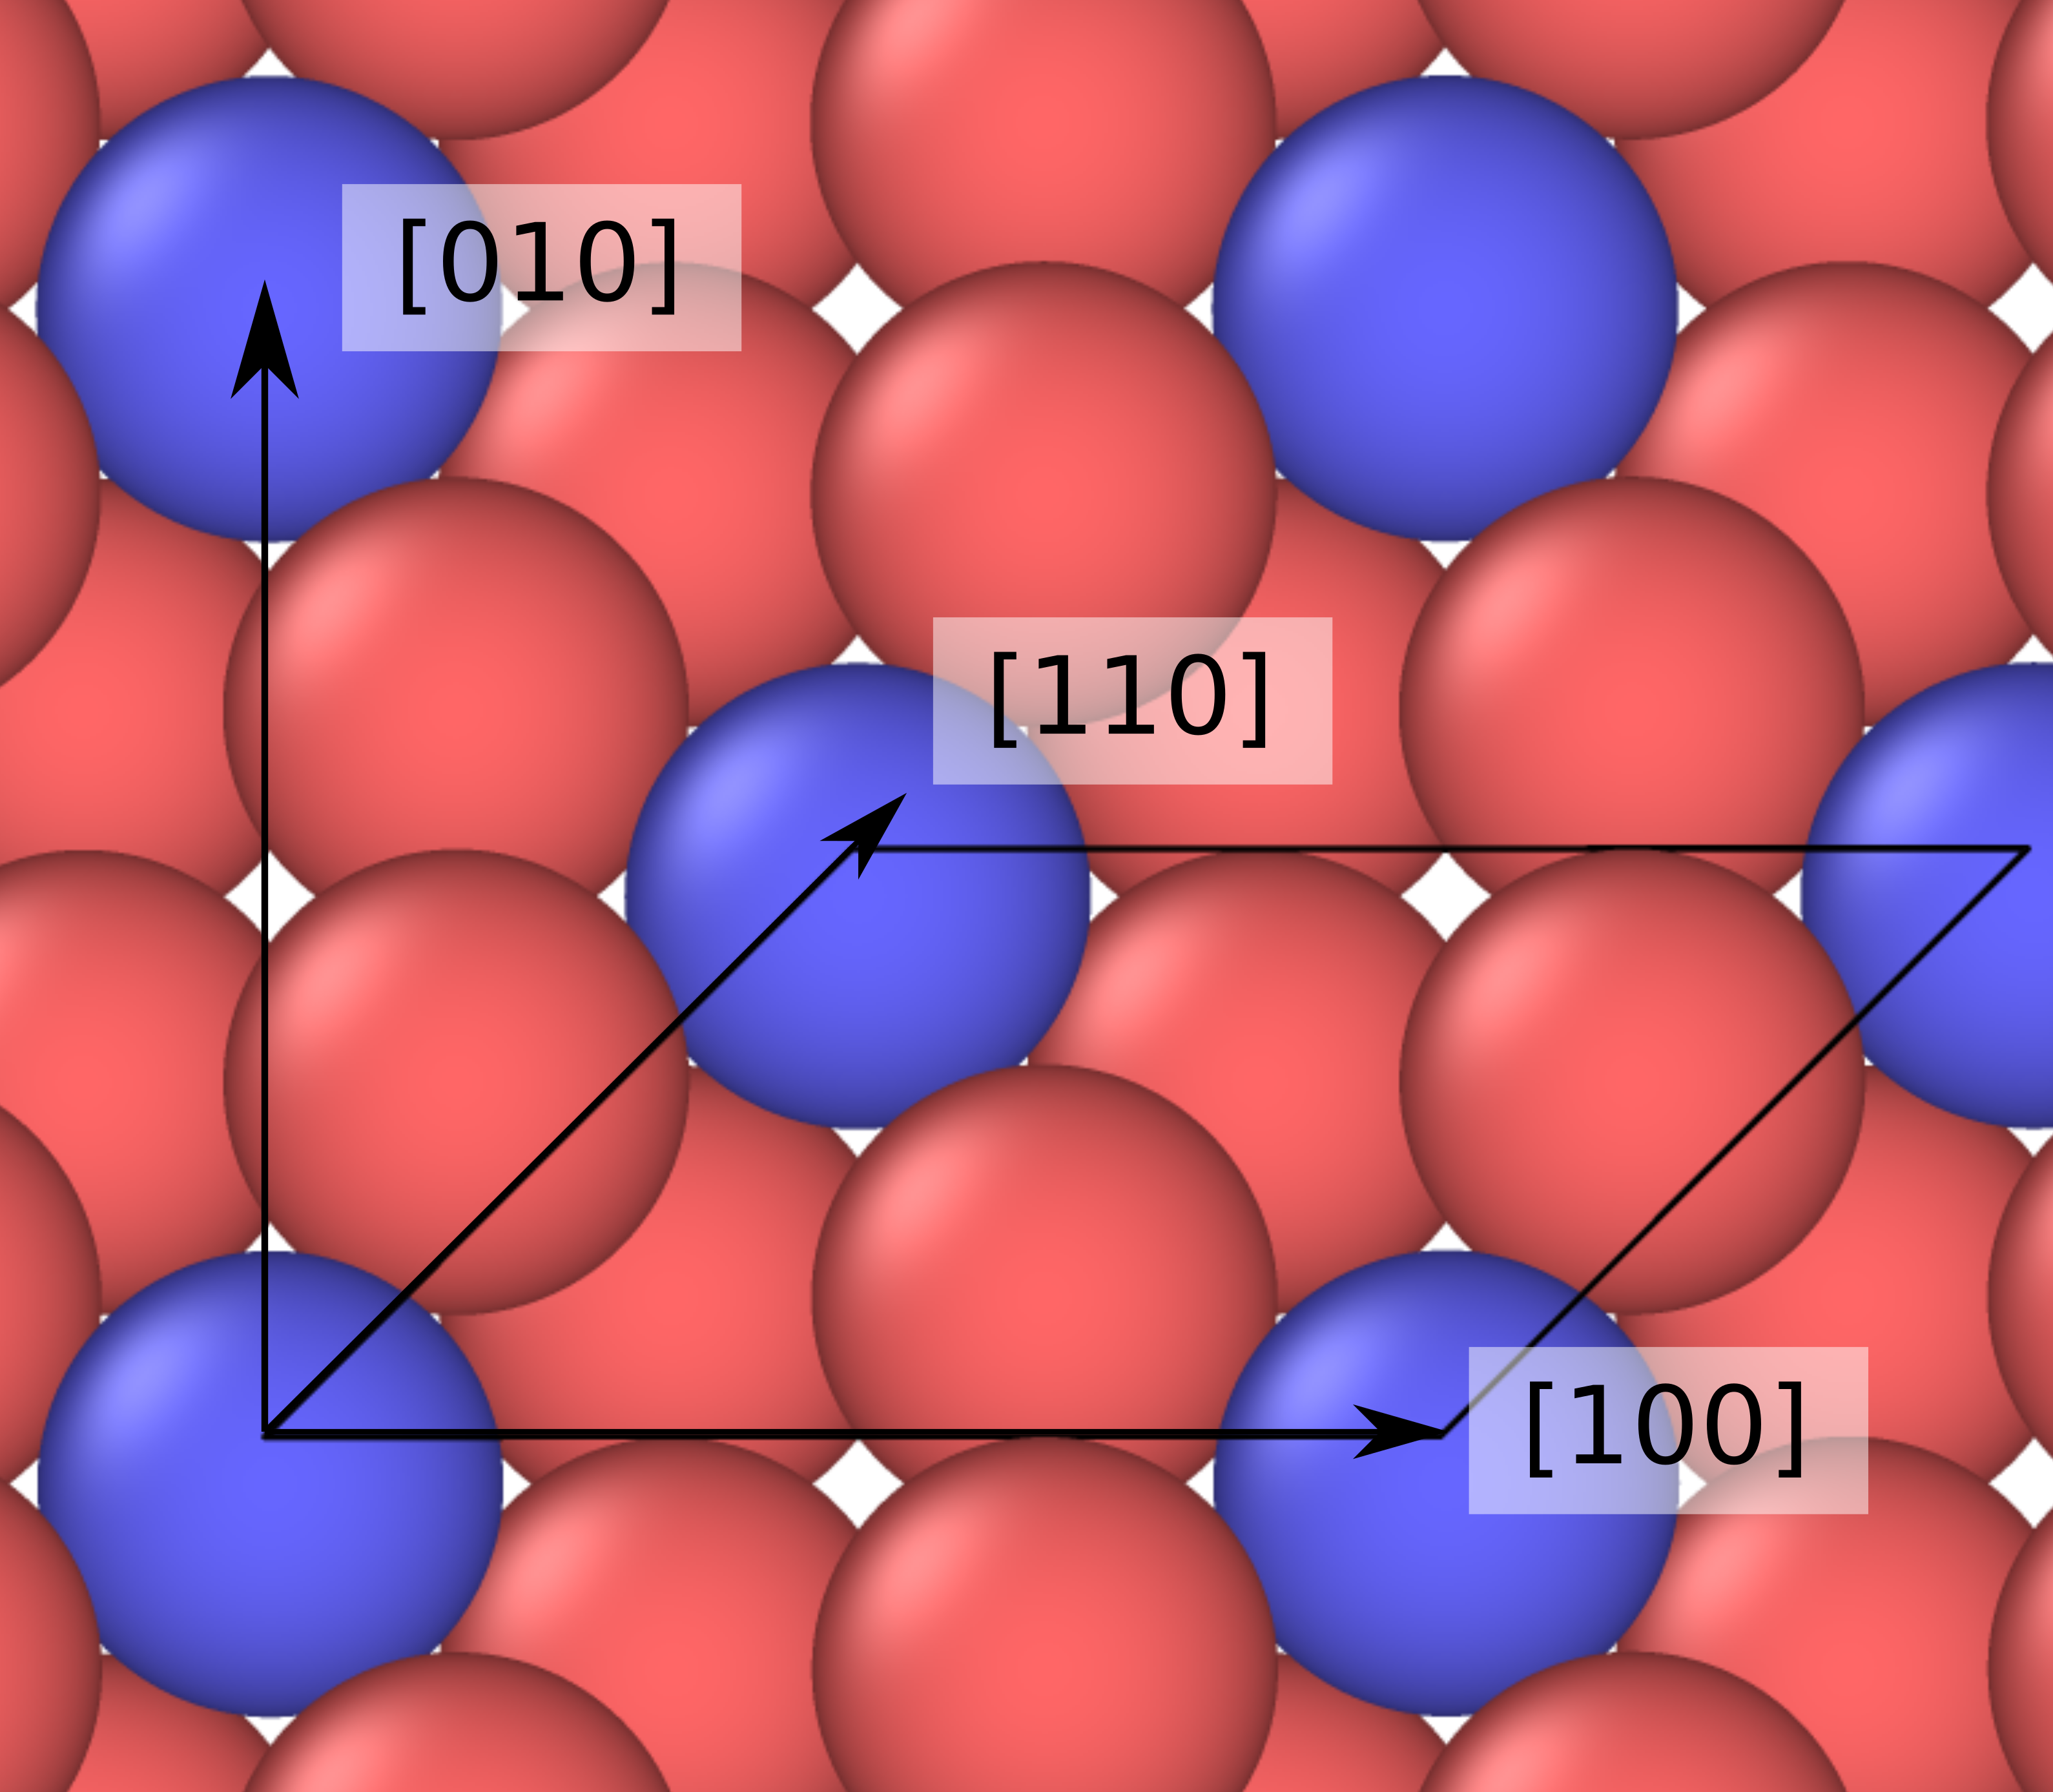
\includegraphics[width=0.40\textwidth]{figures/GSF_Theta0m11_AtomicView.png}
 }}%
\subfloat[]{{
 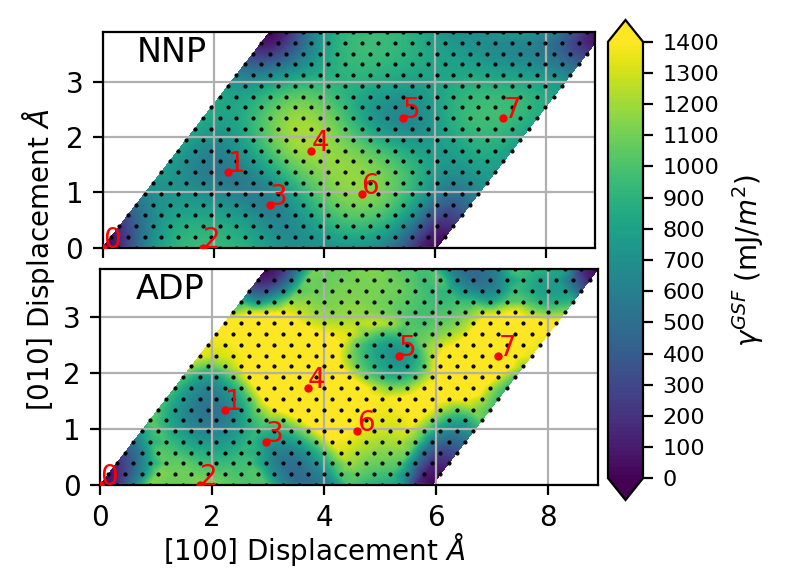
\includegraphics[width=0.60\textwidth]{figures/GSF_Theta0m11_surf.png}
 }}%
\\
\subfloat[]{{
 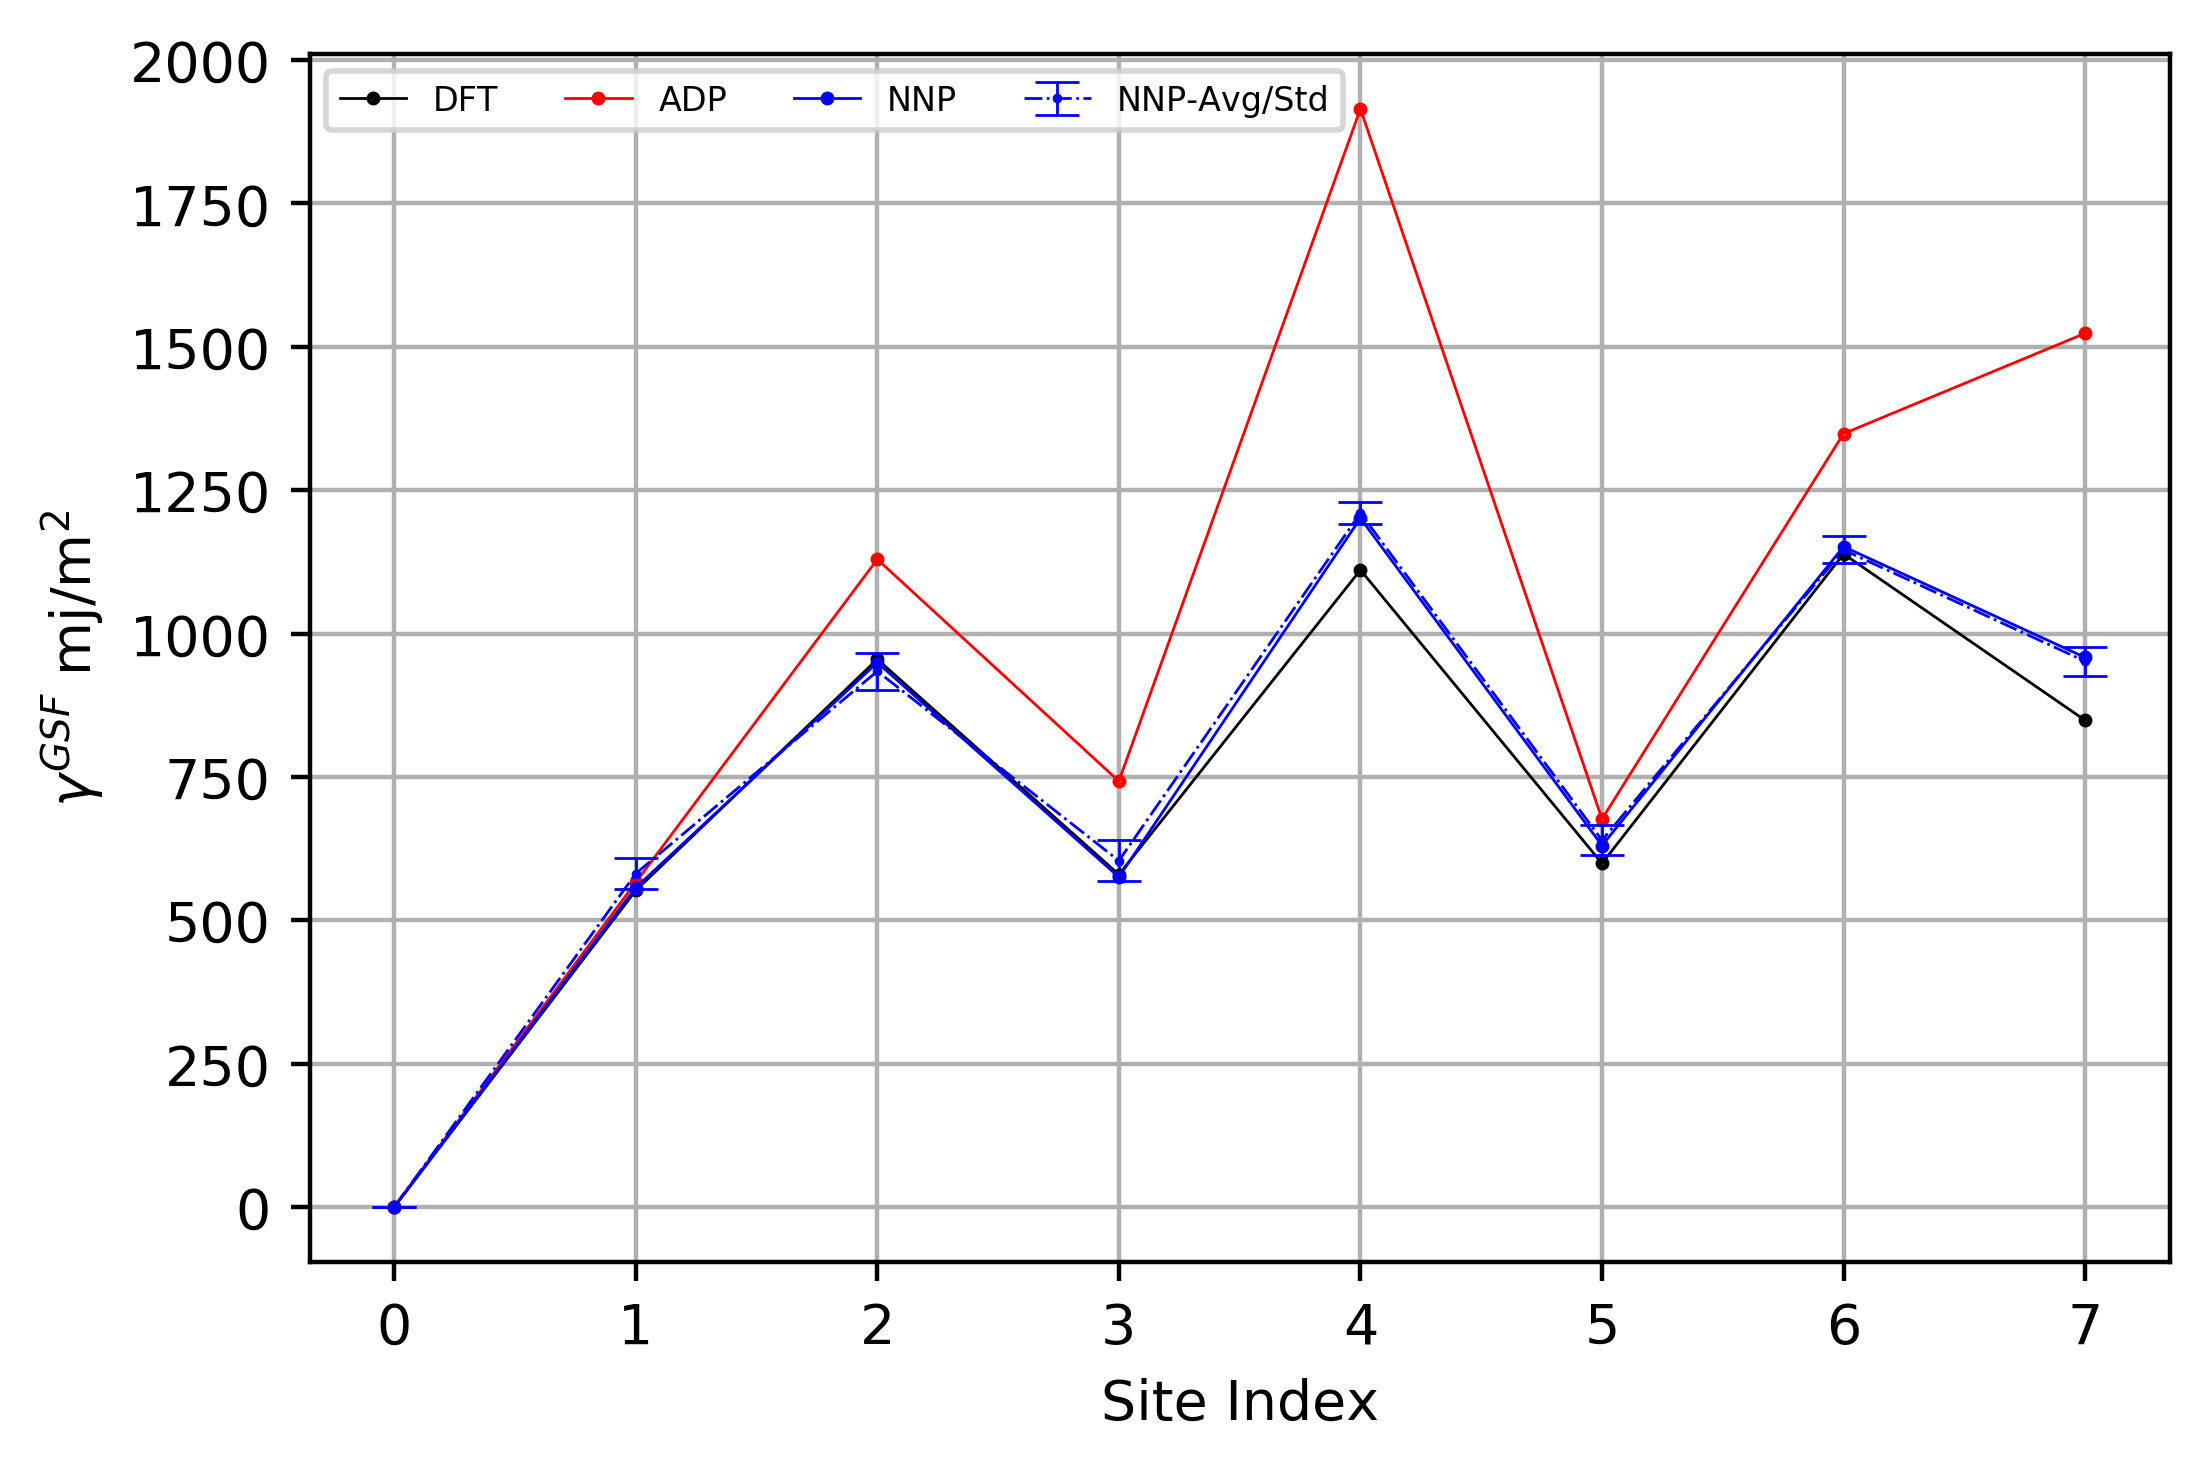
\includegraphics[width=1.00\textwidth]{figures/NOTINOQMD_00001-GSF_0m11.png}
 }}%
\caption{(a) In-plane unit cell for the (0$\overline{1}$1) Generalized Stacking Fault Surface of the $\theta$ precipitate; (b) Generalized Stacking Fault Energy surface as computed by NNP11 and the ADP at a discrete set of points indicated by black dots, from which the energy contour is constructed.  Red points and labels are local minima or maxima for which the energies were computed via DFT and present in the training set; (c) GSFE at the selected extremal points, as computed by DFT (black dots), all the NNPs (blue dashed lines), NNP11 (blue dots), and the ADP (red dots); the structures contributing to the GSFE for these 7 sites are included in the training set.}
\label{fig:GSF_Theta_0m11}
\end{figure}


\section{Results: Validation}

\subsection{Generalized Stacking Faults $\theta''$} \label{sct:gsf_theta_dp}

GP zones and $\theta''$ precipitates are among the most pertinent to understanding mechanical properties of Al-Cu alloys\cite{Nie2014PhysicalAlloys}. 
The most important plane of shearing in the precipitate is then that which most closely corresponds to the (111)-type glide planes of Al.
Both the $\theta''$ precipitates and the GP zones are structurally similar, being composed of (100) planes of Cu in Al. 
The $\theta''$ consists of (100) planes of Cu with one intervening plane of Al spaced by two lattice constants while a GP zone is a single plane of (100) Cu. Here we examine the (111) GSFE surface of $\theta''$ since a GP zone does not have a periodic structure; however, results for $\theta''$ should extrapolate well to GP zones.

Figure \ref{fig:GSF_ThetaDP_111}(a,b) shows the GSFE surface geometry and the energies over the slip surface $\theta''$, as predicted by the NNP and the ADP.  
Even though outside the training set, the NNP predicts a smooth GSFE with maxima and minima at the expected symmetry points.  The ADP prediction is much less smooth, with a lack of radial symmetry around the extremal points and with sharp ridges extending across the high energy regions.
Most troubling is that regions of the ADP-predicted $\theta''$ surface are negative, i.e. the sheared precipitate is more stable than the unsheared precipitate.  The ADP cannot be used reliably to investigate shearing of these precipitates.
Figure \ref{fig:GSF_ThetaDP_111}(c) shows the GSFE energies at the extremal points indicated in Figure \ref{fig:GSF_ThetaDP_111}(b) as predicted by DFT, the NNPs, and the ADP.
The NNPs are in excellent agreement with the DFT results at all points while the ADP is in serious error at several points.
Relative to the GSFE of $\theta$ (0$\overline{1}$1) (Figure \ref{fig:GSF_Theta_0m11}), which was in the training dataset, the accuracy of the NNP is lower and with notably higher variation across the family of NNPs.
Nonetheless, the accuracy remains quite good, validating that these NNPs can be reliable used in complex mechanistically-important environments.
We also note that the NNPs can be further improved by the inclusion of more training data relevant to particular problems of interest, whereas traditional potentials such as the ADP remain high constrained by the limited degrees of freedom available for describing alloys.

\begin{figure}[H]%
\centering%
\subfloat[]{{
 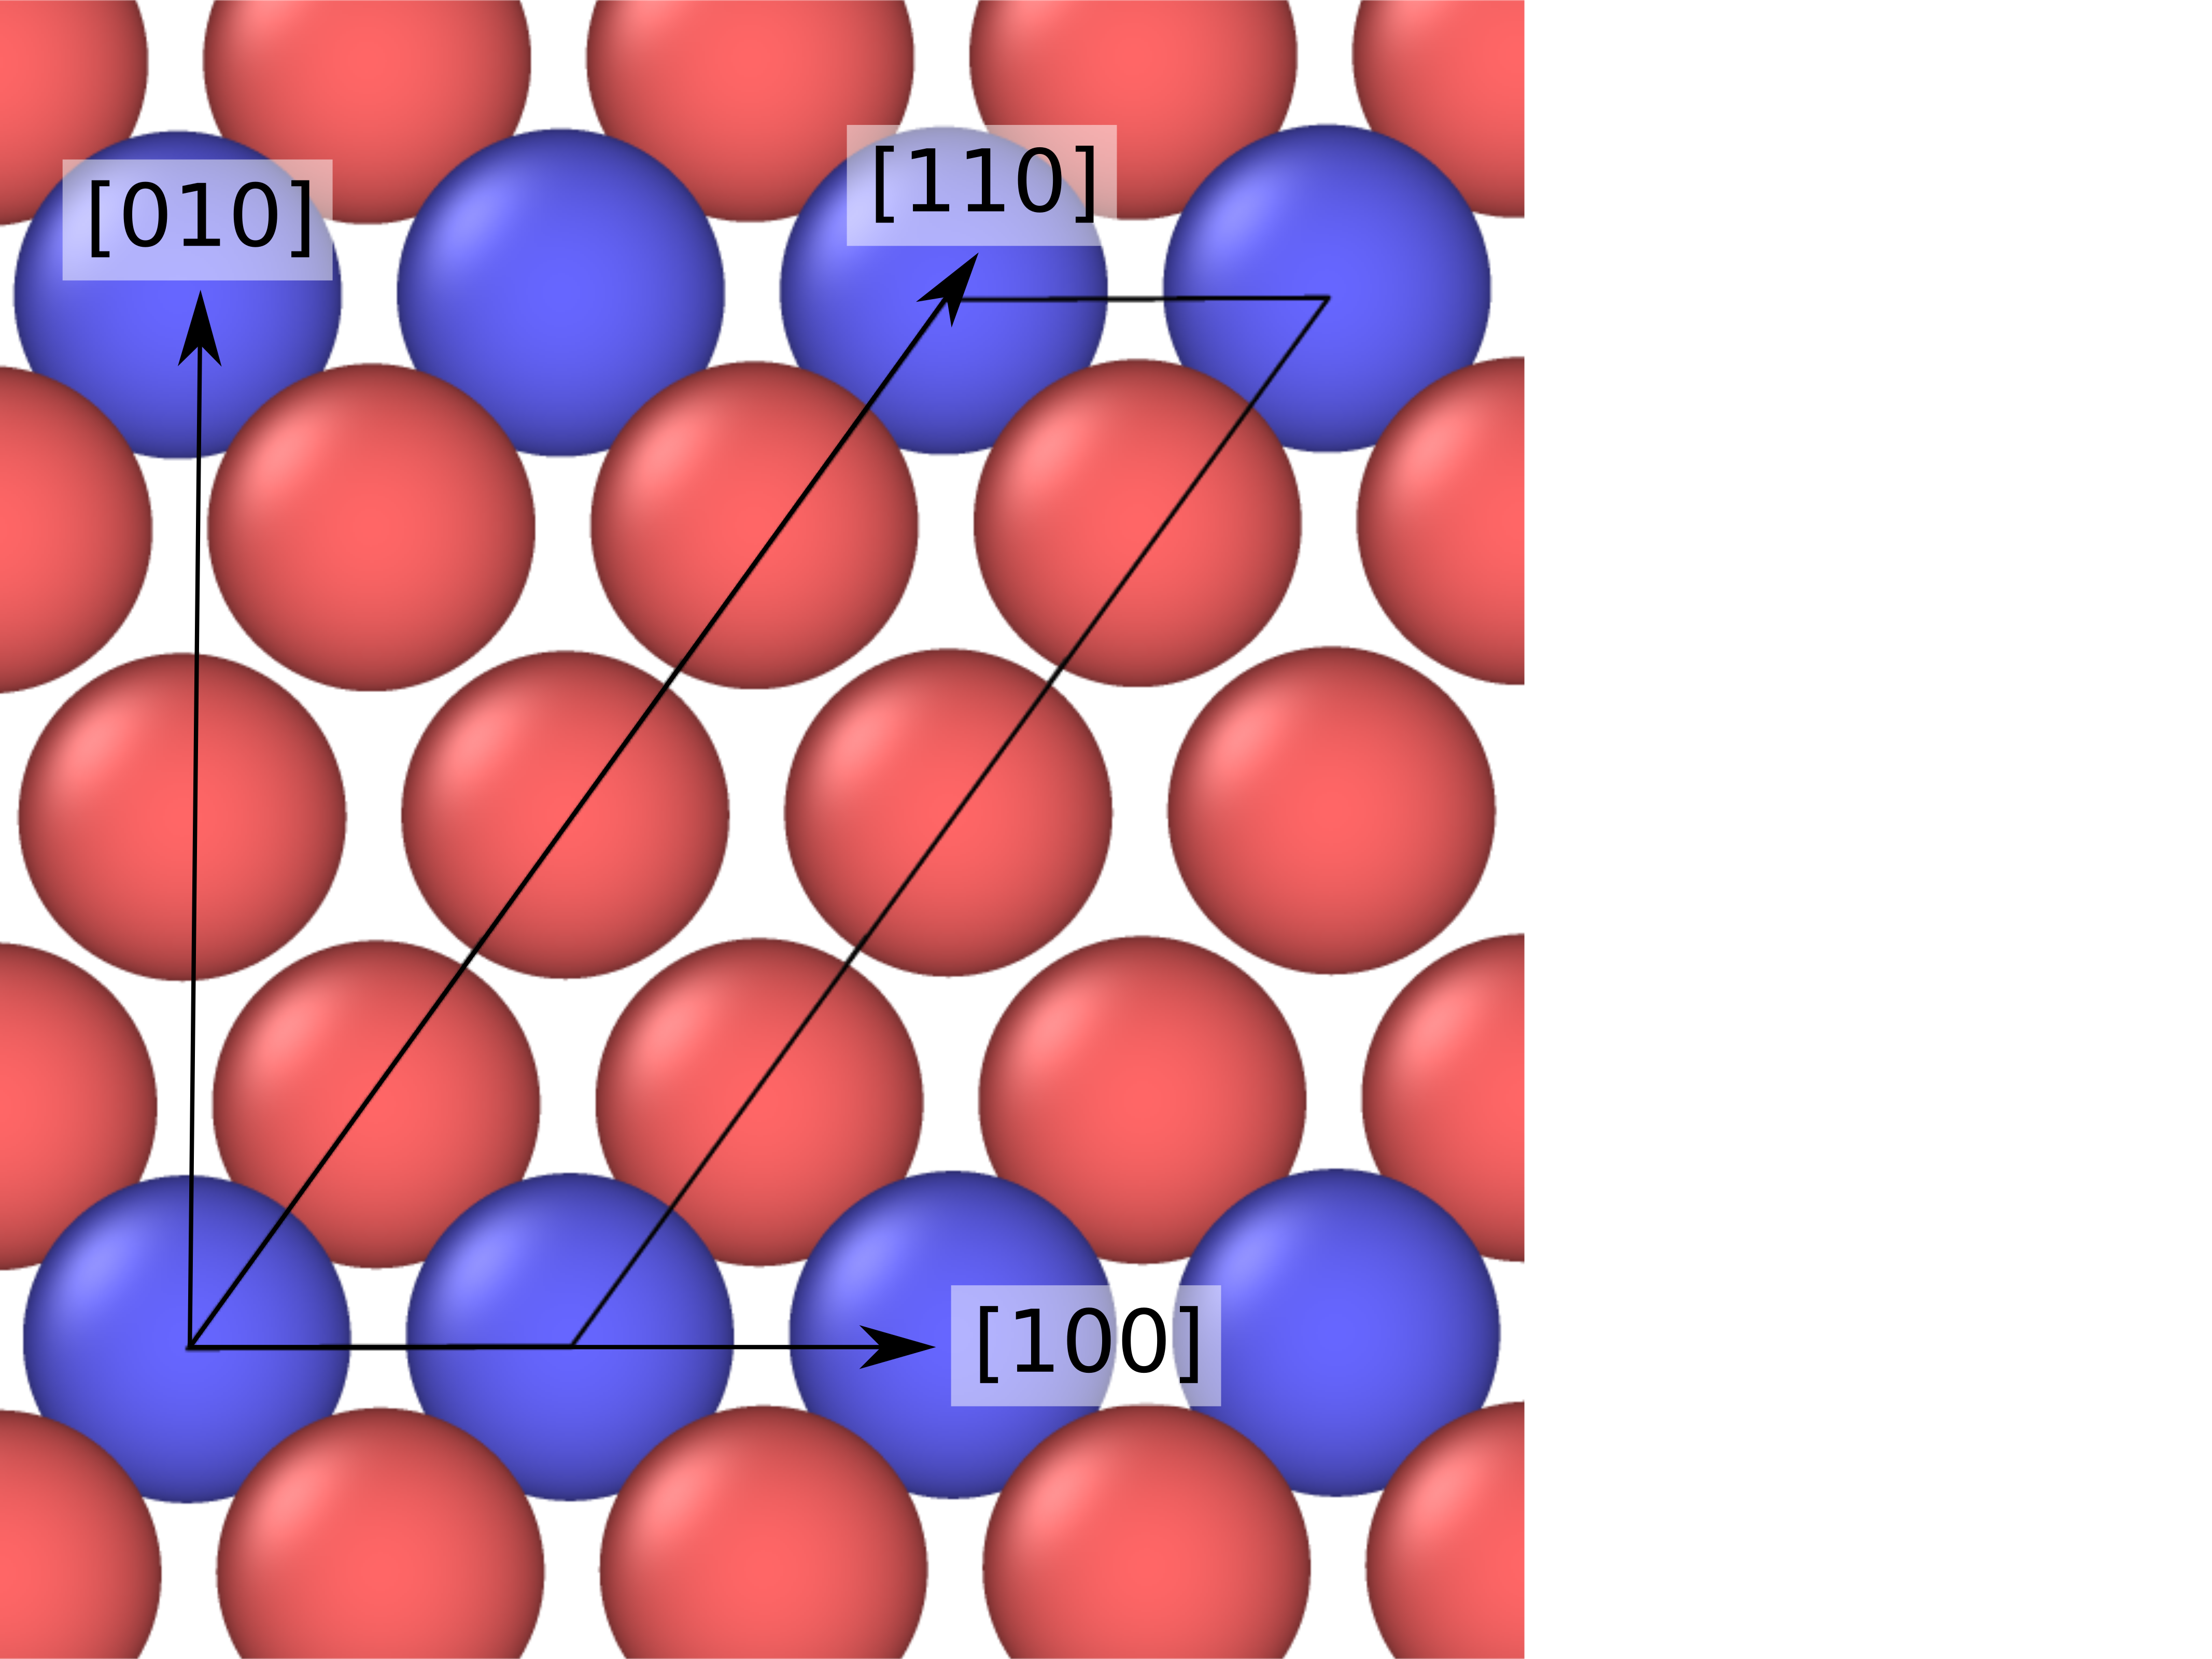
\includegraphics[width=0.32\textwidth]{figures/GSF_ThetaDP111_AtomicView.png}
 }}%
\subfloat[]{{
 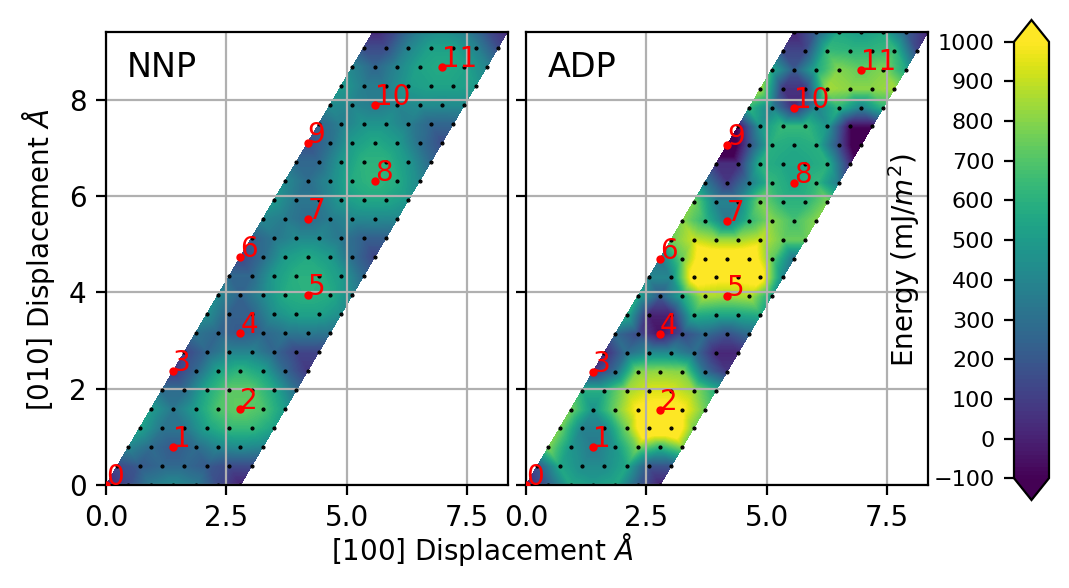
\includegraphics[width=0.68\textwidth]{figures/GSF_ThetaDP111_surf.png}
 }}%
\\
\subfloat[]{{
 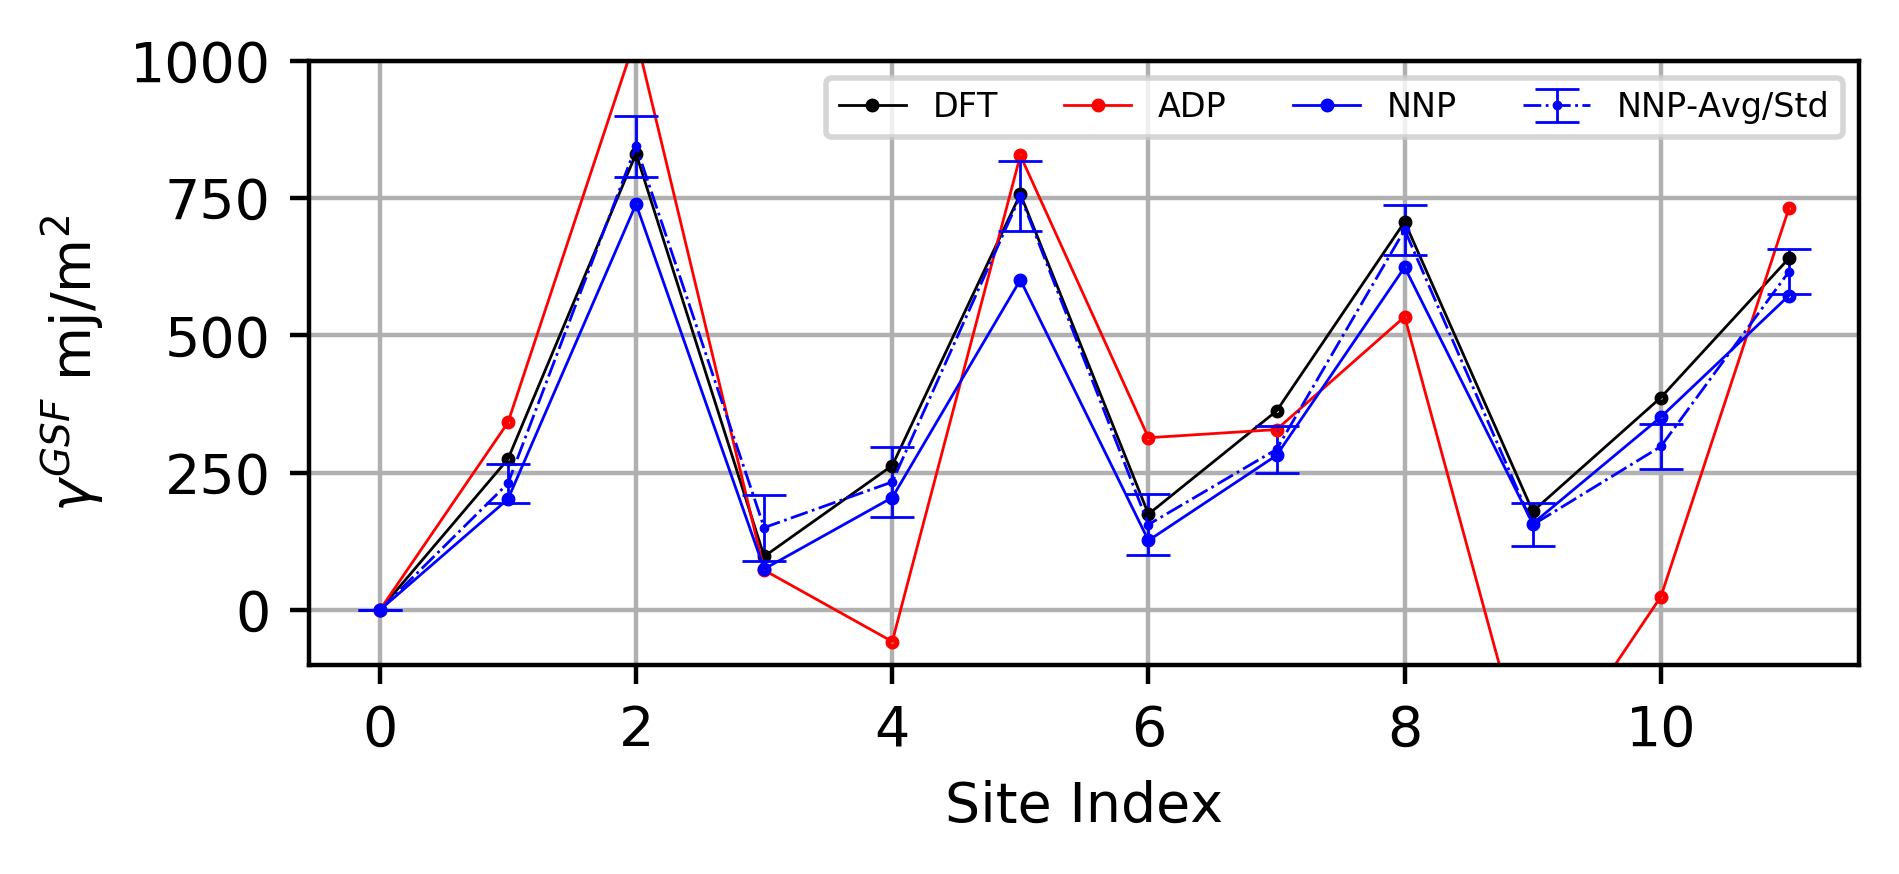
\includegraphics[width=1.00\textwidth]{figures/NOTINOQMD_00002-GSF_111.png}
 }}%
\caption{
In-plane unit cell for the (111) Generalized Stacking Fault Surface of the $\theta''$ precipitate; (b) Generalized Stacking Fault Energy surface as computed by NNP11 and the ADP at a discrete set of points indicated by black dots, from which the energy contour is constructed.  Red points and labels are local minima or maxima for which the energies were computed via DFT and present in the training set; (c) GSFE at the selected extremal points, as computed by DFT (black dots), all the NNPs (blue dashed lines), NNP11 (blue dots), and the ADP (red dots); the structures contributing to the GSFE for these 11 sites are not included in the training set.
}
\label{fig:GSF_ThetaDP_111}
\end{figure}


\subsection{Antisites and Vacancies} \label{sct:antsite_results}

In modeling the evolution of precipitate microstructures, it is unavoidable that there will be anti-site defects and vacancies inside the precipitates.  These configurations also serve as further tests of the ability of the NNPs to broadly capture the energetics of the entire Al-Cu system.
For this reason, we compute the unrelaxed antisite and vacancy formation energies for every OQMD structure predicted to be stable using the NNPs (see Figure \ref{fig:matparam_stats1}). 
Unique atomic sites in each structure were identified using pymatgen.
The primitive unit cell was then used to generate larger cells with a minimum of 108 atoms to minimize defect-defect interactions.
For each of the unique sites identified, a different atom was substituted, e.g. Al $\rightarrow$ Cu or Cu $\rightarrow$ Al, or the atom was removed to create a vacancy.  The unrelaxed formation energies $\Delta E^{antisite}_f$ of all the antisite structures were then calculated relative to the solid solution alloy as
\begin{equation}
\Delta E^{antisite}_f = E^{antisite} - E^{pristine} - E^{ref}_{new} + E^{ref}_{old}
\end{equation}
where $E^{antisite}$ and $E^{pristine}$ are the total energies of the precipitates with and without the antisite defect and $E^{ref}_{new}$, $E^{ref}_{old}$,  are the reference energies for the new and old element respectively, as stated in 
equations \ref{eqn:formRef_Al} and \ref{eqn:formRef_Cu}.

Figure \ref{fig:antisite_plot} shows the antisite results.
%Note that, for clarity of visualization, when there are multiple antisites for a given element and structure, we only display the one with the lowest DFT energy of formation.
When there are multiple possible antisites or vacancies for a given element in a structure, we only plot the one with the lowest DFT formation energy, this is purely to make the figure easier to read, the overall accuracy being the same for all vacancies and antisites. 
For completeness we include Figure \ref{fig:antisite_plot_all} in the supplementary which shows the energies for all antisites and vacancies.
Error bars rarely exceed 0.1eV and are almost always centered around the correct DFT value.
ADP also performs reasonably but has substantially more errors, with many cases deviating by more than 1 eV from DFT.
These results demonstrate that NNPs make accurate predictions of point defects that are not in the training set. 

\begin{figure}[H]%
\centering%
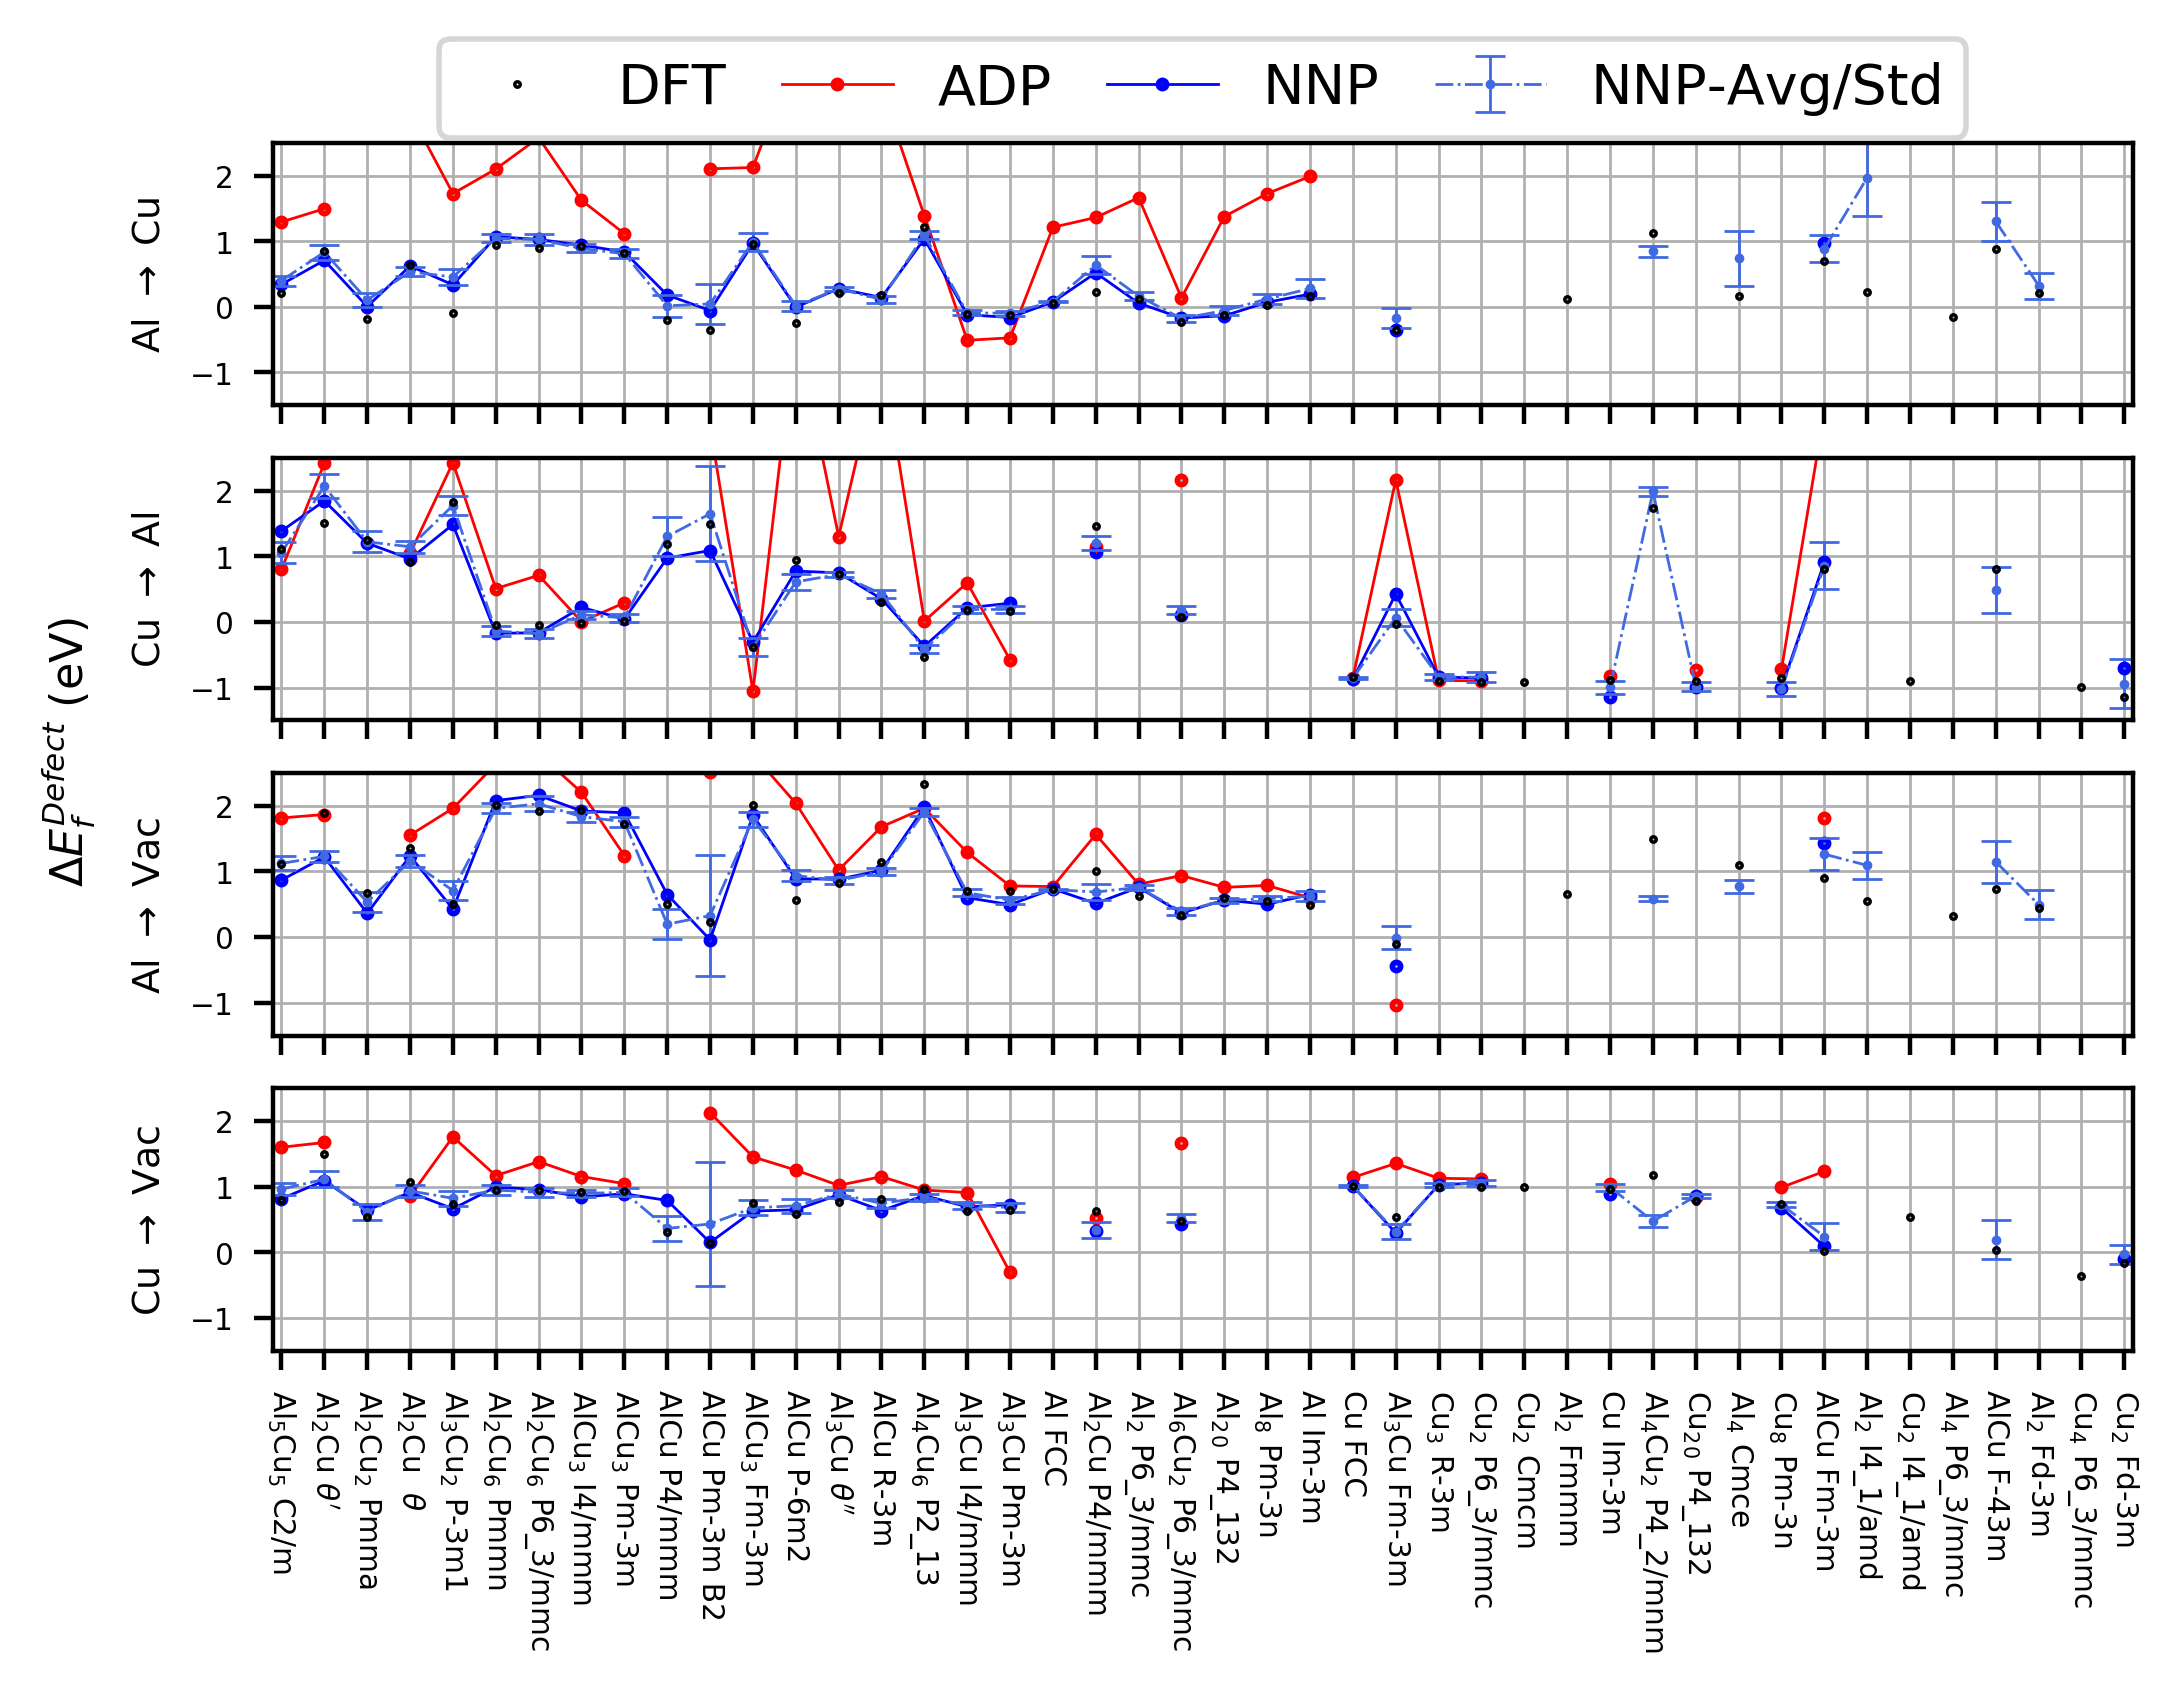
\includegraphics[width=1\textwidth,center]{figures/antisite_vacancies.png}%
\caption{DFT antisite formation energy vs. ADP/NNP antisite formation energy.
These structures were not included in the training set.}%
\label{fig:antisite_plot}
\end{figure}

\subsection{$\theta$ to $\theta'$ transition temperature} \label{sct:thetap_theta_transition}
We now turn to the investigation of the phase transition between the $\theta$ phase and the $\theta'$, comparing the NNPs to the ADP. The T=0K formation energies of both phases have been presented in Figure \ref{fig:matparam_stats1}, and both the NNPs and ADP provide good predictions, with the ADP results also previously reported ~\cite{Apostol2011}. An analysis of the finite-T Gibbs free energy starts with the underlying equations of state of both phases. We therefore fit the T=0K energies to the Vinet equation of state

\begin{eqnarray}
\label{Vinet}
E^{}_{0}(V) &\!\!=\!\!& E^{}_{0}(V^{\rm eq}_0) \;+\; \frac{4B_{T\!,0}V^{\rm eq}_0}{(B_{T\!,0}' -1)^2} \;-\; \frac{V^{\rm eq}_0B_{T\!,0}}{(B_{T\!,0}'
% B^{\rm eq}_0 \text{\begin{minipage}{.3cm}
%  \hspace{.0cm}\Large$'$\vspace{.2cm}
% \end{minipage}}
-1)^2} \:\left\{ 5+3B_{T\!,0}'\left[ \left(\frac{V}{V^{\rm eq}_0}\right)^{1/3}\!\!\!-1 \right]-3\left(\frac{V}{V^{\rm eq}_0}\right)^{1/3} \right\}\nonumber\\[.1cm]
&& \hspace{5.05cm}\text{\Large$\times$} \exp \left\{ -\frac{3}{2}\left(B_{T\!,0}'-1\right)\left[ \left(\frac{V}{V^{\rm eq}_0}\right)^{1/3}\!\!\!-1 \right] \right\},
\end{eqnarray}

with volume $V$, the equilibrium volume at T=0K $V^{\rm eq}_0$, the isothermal bulk modulus $B_{T,0}$ and the pressure derivative of the isothermal bulk modulus $B_{T,0}'$. Table~\ref{albert_tab1} reveals that the ADP potential predicts a large negative value for the derivative $B_{T,0}'$ of the bulk modulus for the $\theta$ phase, which has critical implications for phase stability. The $B_{T,0}'$ values predicted by our neural network differ from the DFT reference for both phases but are positive while the ADP value for the $\theta'$ is in better agreement with DFT.

\begin{table}[H]
    \caption{Derivative of the isothermal bulk modulus $B_{T,0}'$ at T=0K  for the $\theta$ an $\theta'$ phases comparing ADP, DFT, and our neural network.}
\begin{tabular}{lccc}
\hline
\hline
Phase        & ADP (this work)          & DFT        & Neural Network \\ 
\hline 
Theta ($\theta$)        & -4.2      & 4.55     & 2.29  \\
Theta prime ($\theta'$)        & 2.9    & 4.58 & 1.03 \\      
\hline
\hline
\end{tabular}
\label{albert_tab1}
\end{table}


% \begin{table}[H]
%     \caption{Ground state properties for the $\theta'$ phase comparing previously reported ADP results~\cite{Apostol2011} to our calculations using ADP, DFT, and our neural network.}
% \begin{tabular}{lcccc}
% \hline
% \hline
% Property        & ADP~\cite{Apostol2011}             & ADP          & DFT        & Neural Network \\ 
%                 & Apostol et al.        & (this work)  & (this work)& (this work)    \\ 
% \hline 
% a  (\AA)        & 5.649                 & 5.649        & 5.780      & 5.79           \\
% B  (GPa)        & 135.9                 & 136.3        & 94.47      & 96.7           \\
% B' (no units)   & -                     & 2.9          & 4.58       & 1.03           \\ 
% \hline
% \hline
% \end{tabular}
% \label{albert_tab1}
% \end{table}


% \begin{table}[H]
%     \caption{Ground state properties for the $\theta$ phase comparing previously reported ADP results~\cite{Apostol2011} to our calculations using ADP, DFT, and our neural network.}
% \begin{tabular}{lcccc}
% \hline
% \hline
% Property        & ADP~\cite{Apostol2011}             & ADP          & DFT        & Neural Network \\ 
%               & Apostol et al.        & (this work)  & (this work)& (this work)    \\ 
% \hline 
% a  (\AA)        & 5.935                 & 5.935        & 6.056      & 6.037          \\
% c  (\AA)        & 4.908                 & 4.908        & 4.869      & 4.925          \\
% B  (GPa)        & 147.6                 & 146.8        & 99.60      & 114.86         \\
% B' (no units)   & -                     & -4.2         & 4.55       & 2.29           \\ 
% \hline
% \hline
% \end{tabular}
% \label{albert_tab2}
% \end{table}

The full anharmonic Gibbs free energy versus temperature for both $\theta'$ and $\theta$ phases is computed using the methodology in Refs. [~\cite{Grabowski2009,Glensk2015,Glensk2015b}]. We first compute the quasiharmonic Helmholtz vibrational free energies $F^{\rm vib}(T)$ at seven different atomic volumes over the relevant range of volume expansion via direct diagonalization of the force constant matrix to obtain the 3N eigenvectors $\mathbf{k}_i$ and eigenfrequencies $\omega_{i}$ in supercells of N=768 ($\theta$) and N=648 ($\theta'$) atoms.  The vibrational free energy is then
\begin{equation}
    %\nonumber
    F^{\rm vib}(T) = \frac{1}{N} \sum_{i}^{3N} \left[\frac{\hbar\omega_{i}}{2} + k_{\rm B} T \ln\left[1-\mathrm{e}^{- \beta \hbar\omega_{i}}\right]\right],
    \label{Fqh3}
\end{equation}

The Gibbs free energy versus temperature is then computed as.....GIVE THE GENERAL RESULT HERE, PLEASE - THIS IS NOT SPECIFIC TO ADP NOR TO ANY PARTICULAR FITTING OF THE VOLUME CURVES, ETC.  WE ARE NOT TOO INTERESTED IN APPROXIMATE METHODS (E.G. STABILITY OF ADP USING ONLY LINEAR VOLUME EXPANSION).  JUST ADDRESS THE FINAL GIBBS FREE ENERGY, STATING THAT AN EXPANSION UP TO THIRD ORDER WAS USED OR SOMETHING LIKE THAT.  FIGURE PART (A) CAN BE SHOWN, BUT ELIMINATE LINEAR FIT (NOT IMPORTANT), DELETE FIGURE PART (B) (IT REMAINS UNCLEAR WHERE THIS ACTUALLY COMES FROM SINCE THERE ARE NO EQUATIONS SHOWN....) AND FIGURE PART(C) CAN SHOW ONLY THE FINAL RESULTS, WHICH ARE GIBBS FREE ENERGIES VS T FOR BOTH NNP AND ADP UP TO WHATEVER TEMPERATURE ADP IS STABLE.  THIS PAPER IS NOT ABOUT THE ADP SO THIS FIGURE SHOULD SHOW BOTH ADP AND NNP RESULTS, OR JUST SHOW NNP RESULTS FOR FIGURES (A) AND (B) AND THEN FINAL RESULTS FOR BOTH NNP AND ADP IN FIGURE (C).  THEN COMMENT ON THE FIGURE - ADP THETA IS UNSTABLE BEYOND XXX K WHILE THE NNP11 SHOWS A TRANSITION AT YYY K.
YOU CAN COMMENT THAT PREVIOUS ADP ANALYSIS USING A LINEAR APPROXIMATION SUGGESTED THETA WOULD BE STABLE BUT THAT THE FULL ANHARMONIC ANALYSIS SHOWS THE LINEAR RESULT TO BE INCORRECT - THIS IS ABOUT ALL THAT NEEDS TO BE SAID.

\begin{figure}[H]
    %\includegraphics[width=\columnwidth]{../bilder/phase_transition-crop.pdf}
    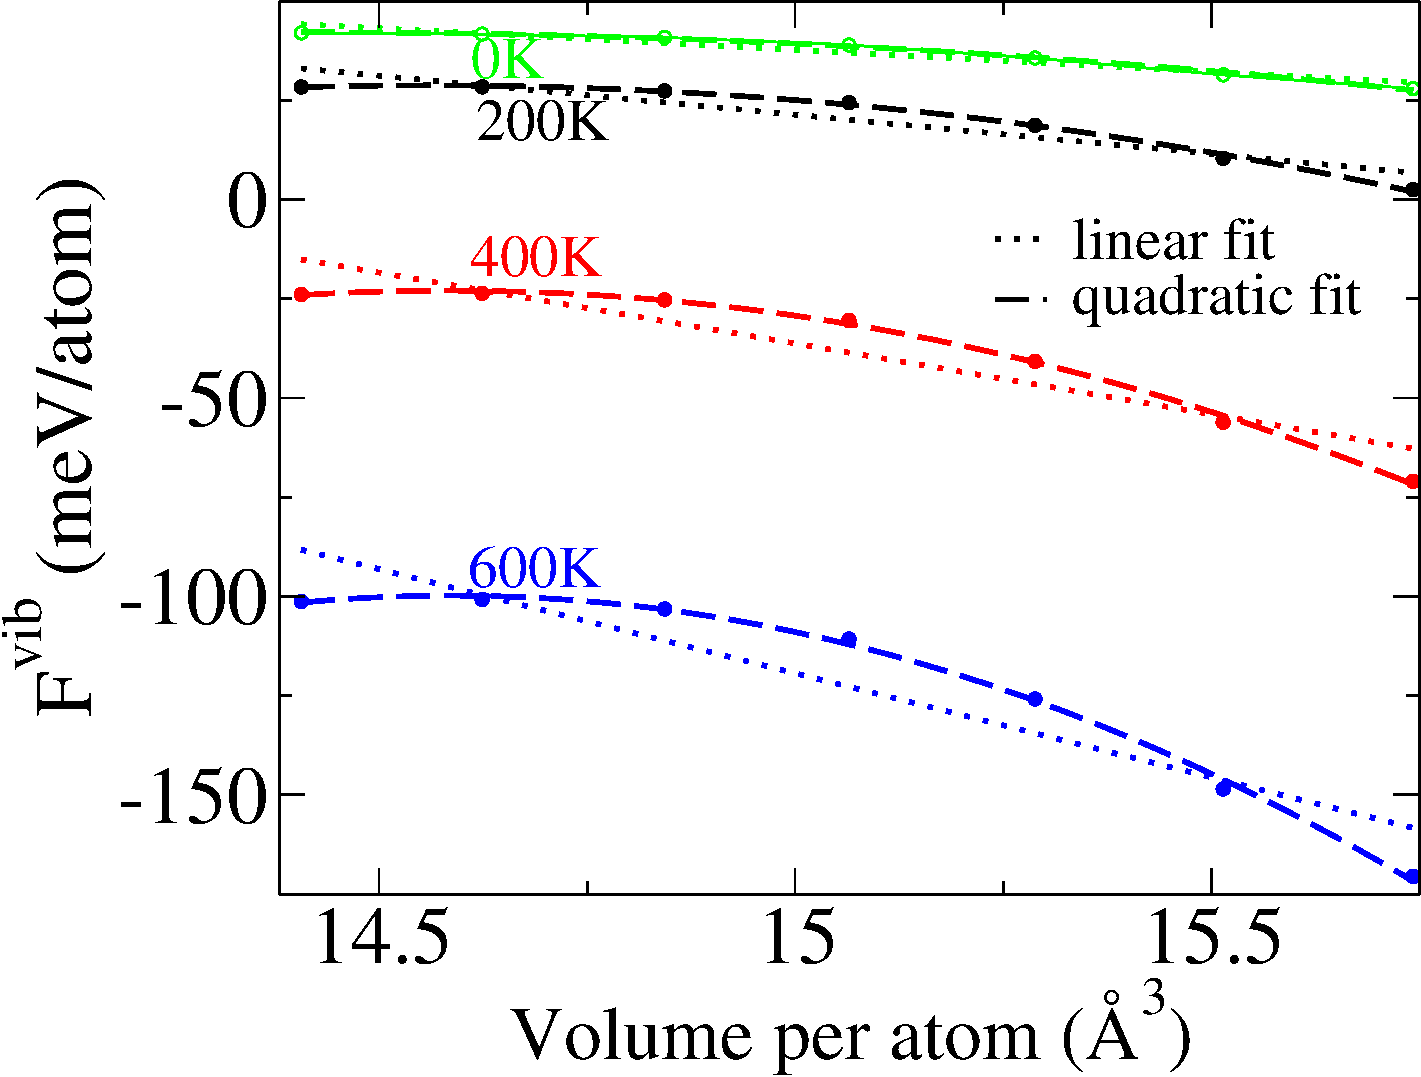
\includegraphics[width=0.5\columnwidth]{albert_figures/Fvib_vs_Volume-crop.pdf}
    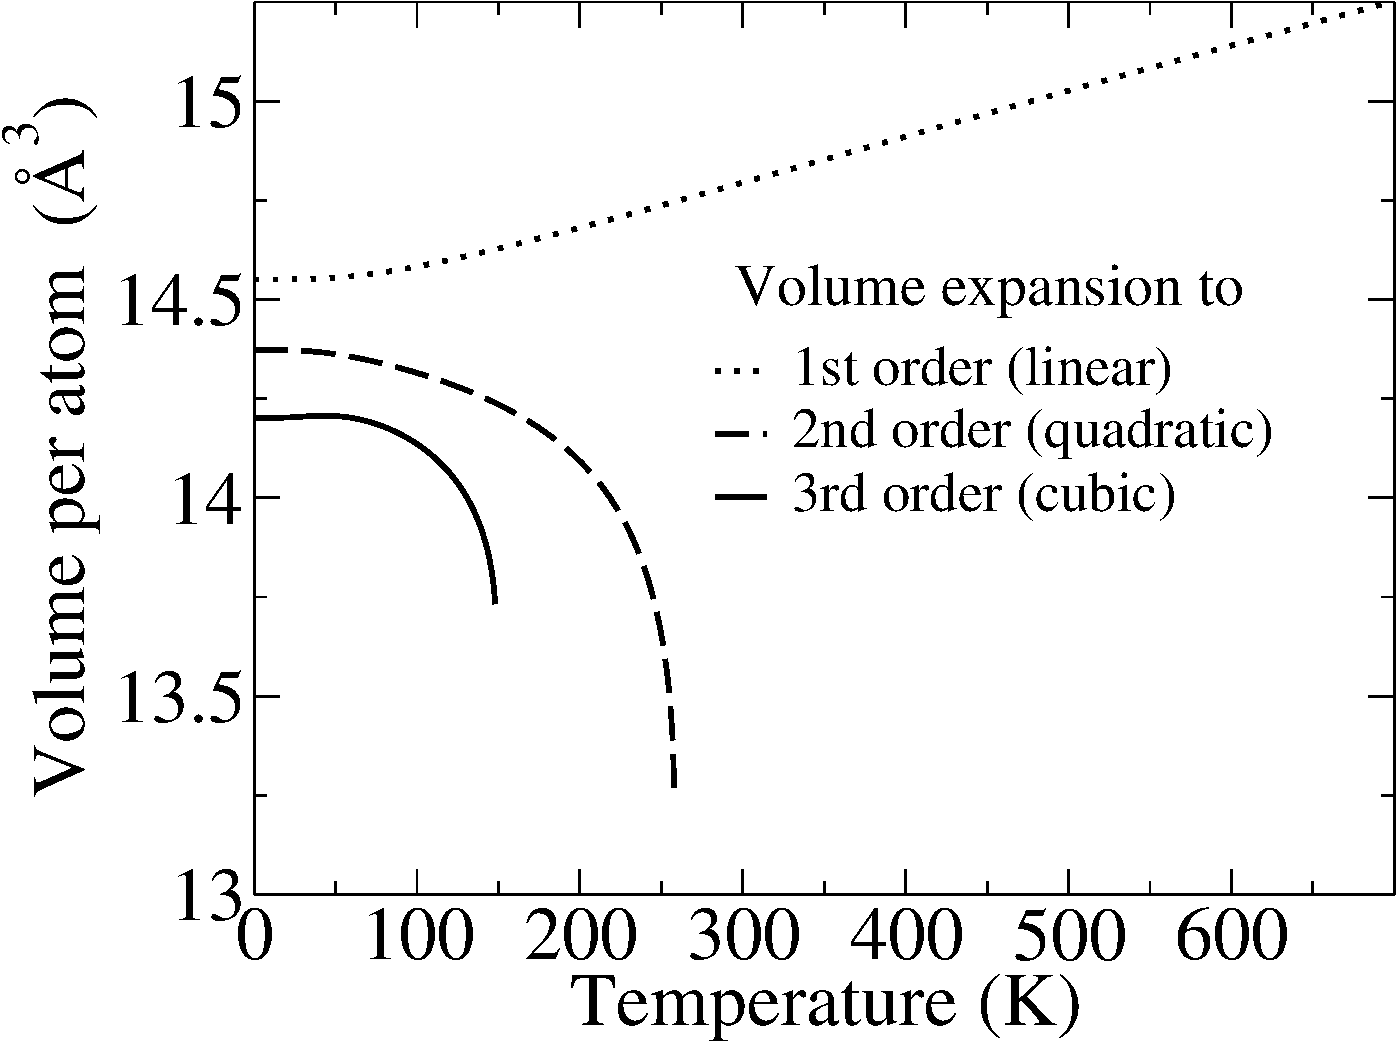
\includegraphics[width=0.5\columnwidth]{albert_figures/volume_expansion-crop.pdf}
    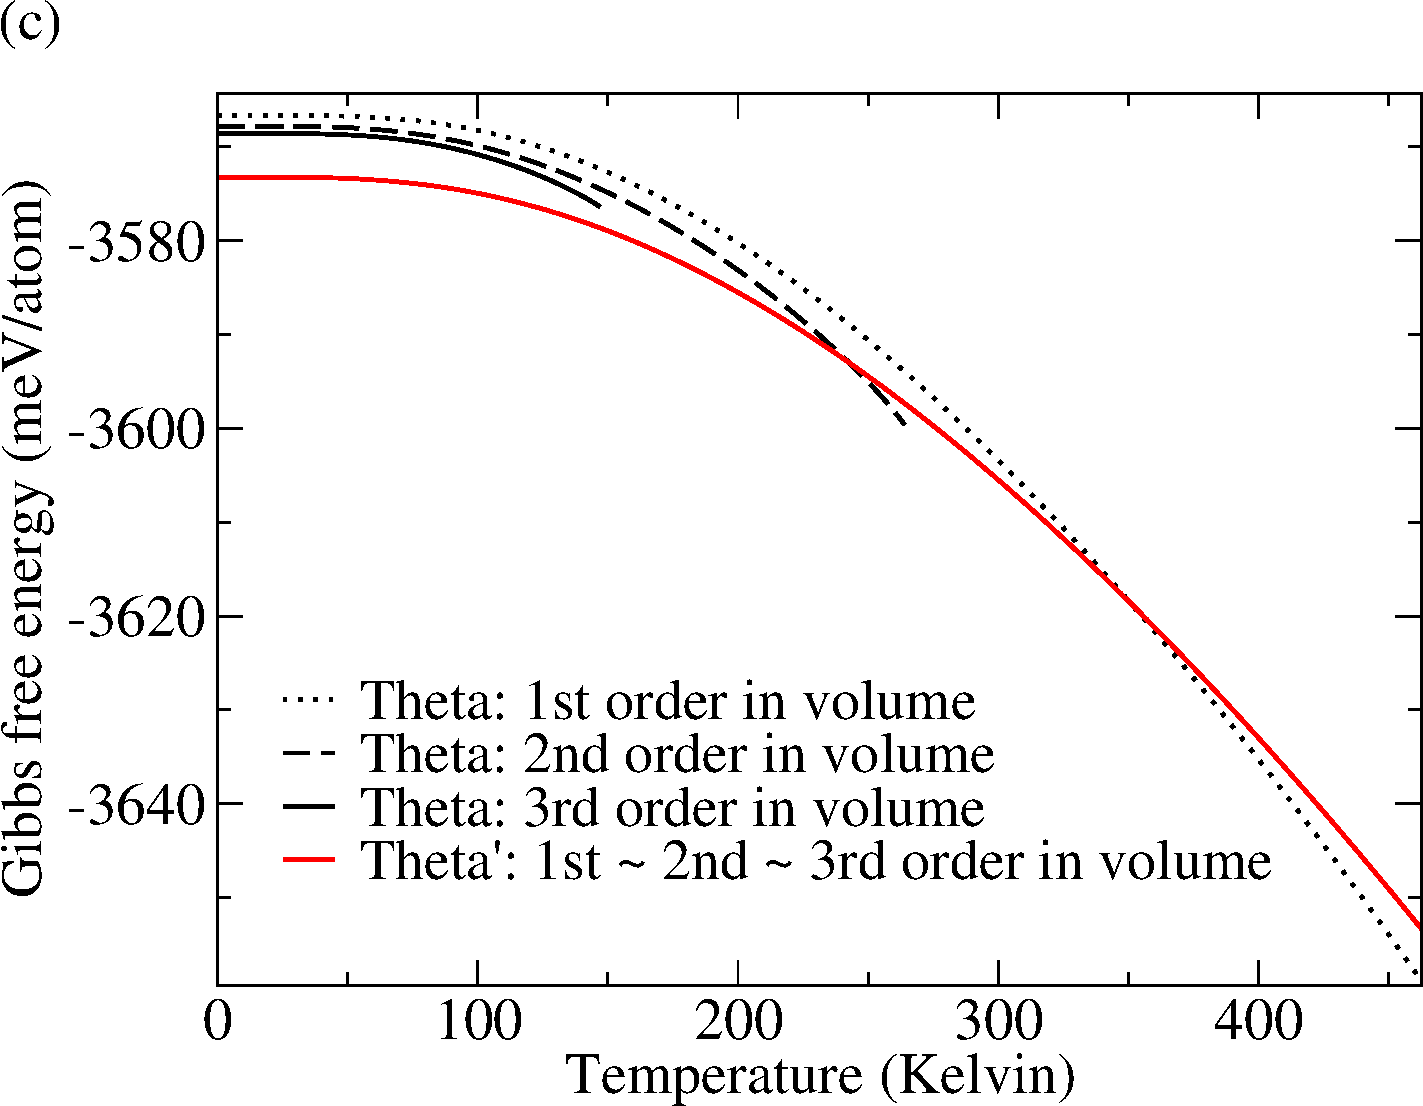
\includegraphics[width=1.0\columnwidth]{albert_figures/summary_phase_transition-crop.pdf}
    \caption{Results for the $\theta$ phase using the ADP potential. (a) Vibrational free energies $F^{\rm vib}(T)$ at different volumes (full circles) obtained at 0~K, 200~K, 400~K and 600~K. The dotted (dashed) lines are interpolations using linear (quadratic) polynomials. (b) Volume expansion of the $\theta$ phase applying the linear (dotted), quadratic (dashed) and cubic polynomials (solid line) for the volume dependence of the free energy surface. (c) Gibbs free energies as function of temperature for the $\theta$ phase (black) and for $\theta'$ (red) using different extrapolations for the volume.} 
    \label{fig1}
\end{figure}




\begin{figure}[H]
    %\includegraphics[width=\columnwidth]{../bilder/phase_transition-crop.pdf}
    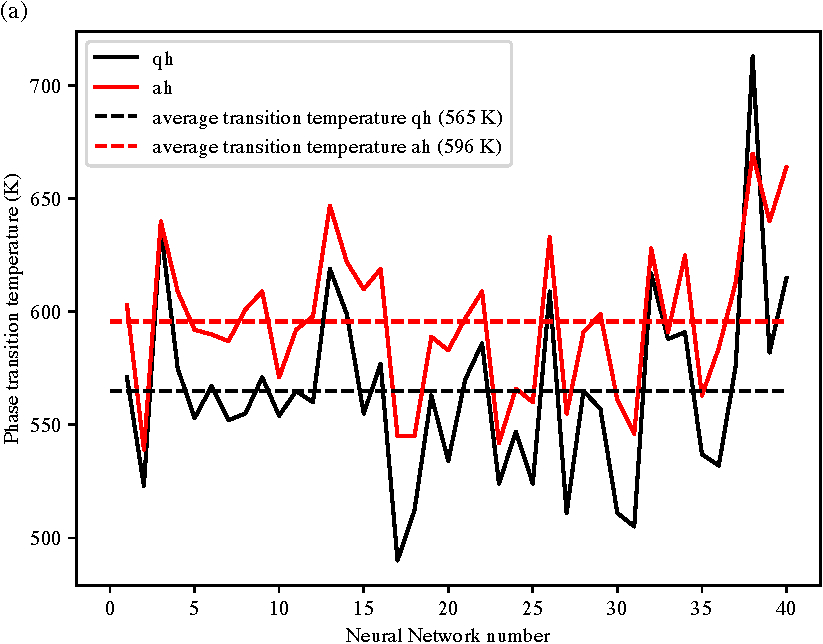
\includegraphics[width=\columnwidth     ]{albert_figures/alle-crop.pdf}
    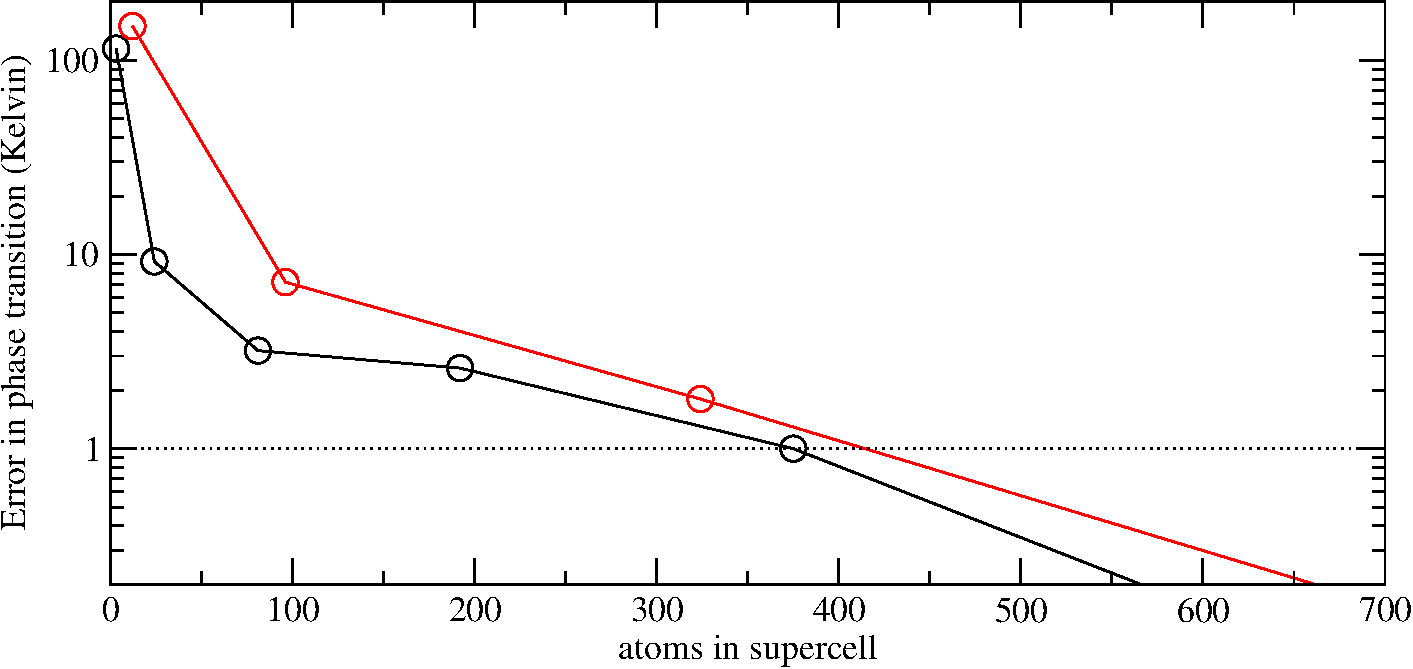
\includegraphics[width=0.5\columnwidth]{albert_figures/convergence_atoms_in_supercell-crop.pdf}
    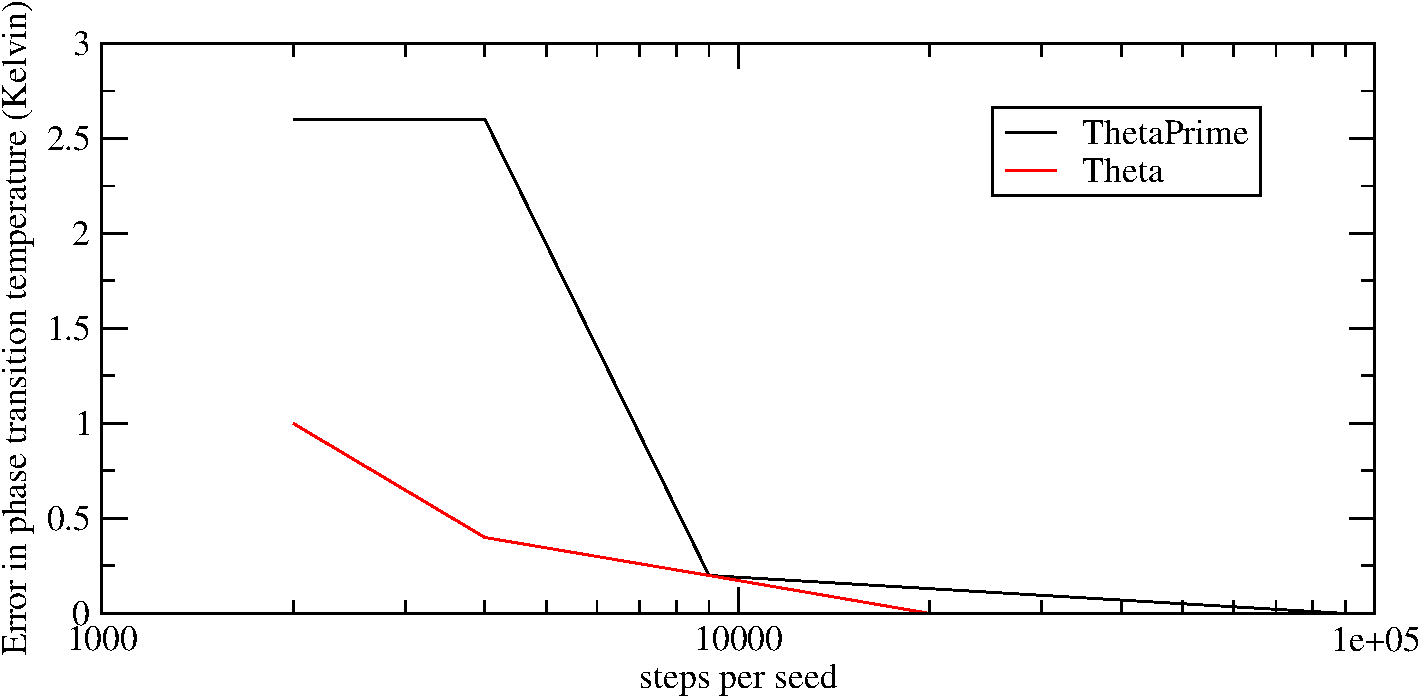
\includegraphics[width=0.5\columnwidth ]{albert_figures/convergence_steps-crop.pdf}
    \caption{(a) Phase transition temperature between $\theta$ and $\theta'$ as obtained by 40 neural network potentials trained with different initial random seed, in quasiharmoinc approximation (black) and taking the full anharmonicity into account (red). Averages are indicated by the corresponding dotted lines. (b)  } 
    \label{fig2}
\end{figure}

NOW I AM CONFUSED.  I AM REALLY ONLY INTERESTED IN SHOWING THE FULL ANHARMONIC RESULT. SO, JUST DESCRIBE HOW THAT IS DONE, CLEARLY BUT CONCISELY. ALL OF THE METHODS AND ANALYSIS ARE ENTIRELY IN THE LITERATURE AND NEED NOT BE REPEATED HERE. 
We now analyze the quasiharmonic (qh) phase transition temperature as predicted by our neural network potential and assess in a first step the variance due to the initial random seed of training. To this end, we calculate the full quasiharmonic free energy surface and the resulting phase transition temperature for 40 different neural network potentials. The different transition temperatures are shown in Fig.~\ref{fig2}~(a) (black solid line) with an average phase transition temperature of 565~K (dashed solid line) with a standard deviation of 33~K. We find that ---in contrast to the ADP potential--- all investigated potentials are stable in quasiharmonic approximation up to the tested 1400~K. 

In order to obtain the phase transition temperature including the full anharmonic interactions, we perform thermodynamic integration~\cite{Grabowski2009,Glensk2015}. Corresponding convergence tests, shown in Figs.~\ref{fig2}(b) and (c), reveal that supercells containing 96 and 81 atoms ---for the $\theta$ and $\theta'$ phases respectively--- give rise to small numerical errors in the phase transition temperature of about 10~K, while the largest considered cells (768 and 648 atoms) show negligible numerical errors of less than 1~K. To obtain the anharmonic corrections to the free energy, we perform molecular dynamics calculations with 1~fs time step at seven volume and seven temperature points along the thermodynamic path connecting the quasiharmonic to the fully anharmoinc free energy surface. At every temperature and volume point we run molecular dynamics at five coupling parameters and average over three molecular dynamic runs. The corresponding numerical errors are when using 9000 time steps per molecular dynamics run are less than 1~K as show in Figs.~\ref{fig2}(c) and therefore sufficient for our purpose. Taking the full anharmonicity into account, the phase transition temperature is raised by 31~K to 696~K (with a standard deviation of 5~K).

FIGURES FOR THIS SECTION WILL BE SIGNIFICANTLY REDUCED IN NUMBER AND CONTENT.  QH RESULTS NOT NEEDED, PER ABOVE....


\subsection{Solute Clusters and Kinetic Monte Carlo (KMC)} \label{sct:solute_clusters_KMC}

In early-stage precipitation, pre-precipitates are nucleating by formation of small multi-atom clusters.  An understanding of the nucleation and early-stage growth thus requires that a potential properly represent not only many possible precipitate phases and precipitate/matrix interfaces but also possible clusters that cannot be classified as precipitates.  The pair interactions have already been discussed, and so here we focus on several 3 and 4 atom clusters of Cu in Al that have recently been studied by \cite{Gorbatov2019EffectiveAlloys} et al. in their development of a cluster expansion method.  The specific clusters are illustrated in Table \ref{table:solute_cluster} and we use the notation of Gorbatov et al.  Among these clusters, we note that the 111 and 111111 (compact triangle and tetrahedron of nearest neighbor Cu atoms, respectively) are not compatible with the formation of GP-I and GP-II zones on the (100) planes that occur in real Al-Cu while the 112, 111112, and 111122 clusters are consistent with GP-I and GP-II zones.

We compute the cluster formation energy $\Delta E^{cluster}_{f,(N-X,X)}$ as the energy of the embedded cluster relative to the energy of Cu in solid solution,
\begin{equation}
\Delta E^{cluster}_{f,(N-X,X)} = E^{cluster}_{N-X,X} - \sum_i E^{ref}_i
\end{equation}
The DFT values for all the clusters as computed in simulation cells of 256 atoms are shown in Table \ref{table:solute_cluster} along with the NNP and ADP values.  The DFT predicts that clusters favoring the (100) plane are energetically preferable as compared to the other clusters and with the 111111 tetrahedron cluster having positive formation energy.  NNP11 is in reasonable agreement with DFT for most of the clusters, but notably incorrectly predicts a strongly negative formation energy for the 111111 cluster and also over-predicts the stability of the 111 cluster.  NNP10, also shown, is in better agreement with DFT with respect to the relative stability of the clusters.  Across the mean and standard deviation of the 40 NNPs, the deviations seen for NNP11 are also not evident.  The ADP potential shows gross errors, predicting all clusters to be very energetically favorable and predicting the relative stability of the 3-atom clusters incorrectly (as does NNP11 but with a much smaller difference).  Application of ADP to the study of early-stage clustering is thus expected to be very inaccurate while the performance of the NNPs may vary.  We will investigate this next.

IN TABLE 4, NEED TO ADD ADP RESULTS FOR UNRELAXED 4- AND 10- ATOM TETRAHEDRAL CLUSTERS.
%
%\begin{figure}[H]%
%\centering%
%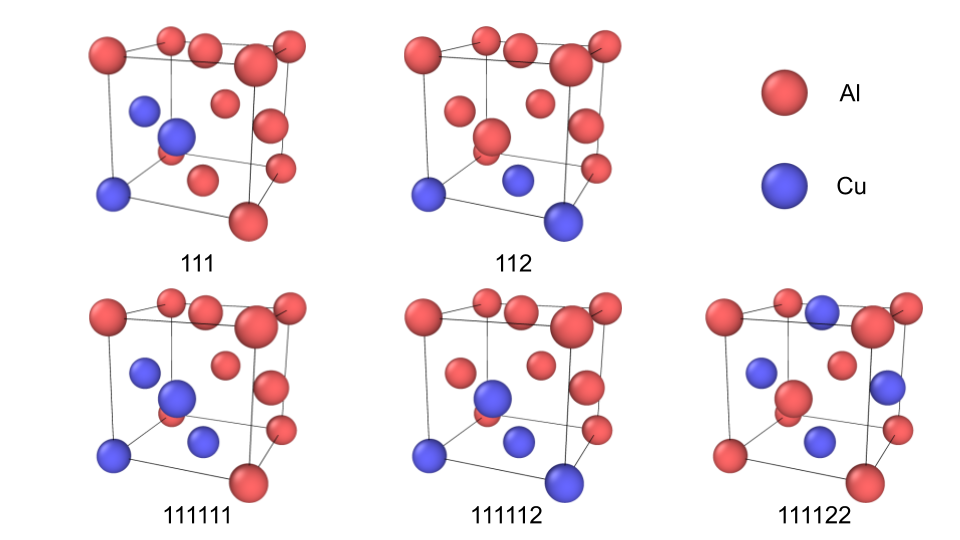
\includegraphics[width=1\textwidth,center]{figures/ClusterPlot-Daniel-2020.04.15.png}%
%\caption{Three and four atom clusters considered in this study. 
%Clusters are described using the the length of edges of the cluster, e.g., 111 represents three edges all nearest neighbors. Note that there are three edges for a three atom cluster but six edges for a four atom cluster.}%
%\label{fig:atomview_clusters}
%\end{figure}

\begin{table}[H]
\begin{tabular}{l|cccccV}%
\hline%
&DFT&ADP&NNP11& NNP10& NNP-\emph{Avg / StdDev} & Figure \\%
\hline%
\hline%
&&&&&& \\
$E^{3Cu}_{111}$ (eV)&-0.073&{-}0.718&{-}0.112& -0.096 &\emph{-0.060 / 0.037}  & 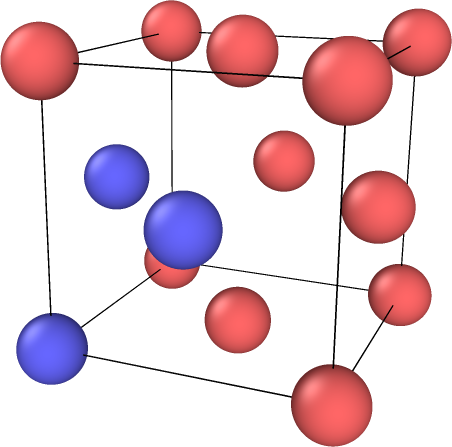
\includegraphics[width=0.07\textwidth]{figures/SoluteCluster_111.png}  \\%
$E^{3Cu}_{112}$ (eV)&-0.112&{-}0.595&{-}0.097& -0.127 &\emph{-0.085 / 0.025}  &  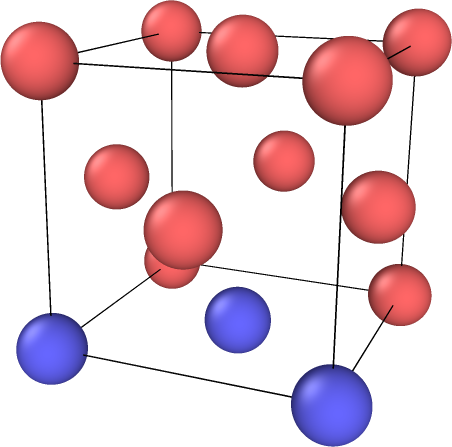
\includegraphics[width=0.07\textwidth]{figures/SoluteCluster_112.png}\\%
$E^{4Cu}_{111111}$(eV)&0.039&{-}0.612&{-}0.081& -0.003 &\emph{0.071 / 0.086}  &  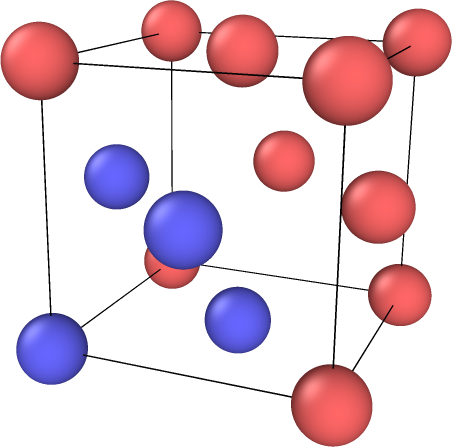
\includegraphics[width=0.07\textwidth]{figures/SoluteCluster_111111.png}\\%
$E^{4Cu}_{111112}$(eV)&-0.126&{-}1.071&{-}0.184& -0.183 &\emph{-0.093 / 0.066}& 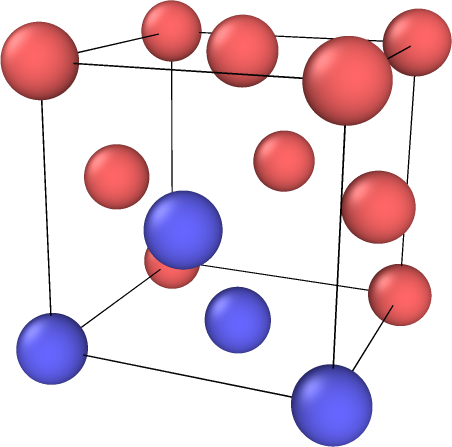
\includegraphics[width=0.07\textwidth]{figures/SoluteCluster_111112.png} \\%
$E^{4Cu}_{111122}$(eV)&-0.268&{-}1.275&{-}0.226& -0.312 &\emph{-0.205 / 0.055}&  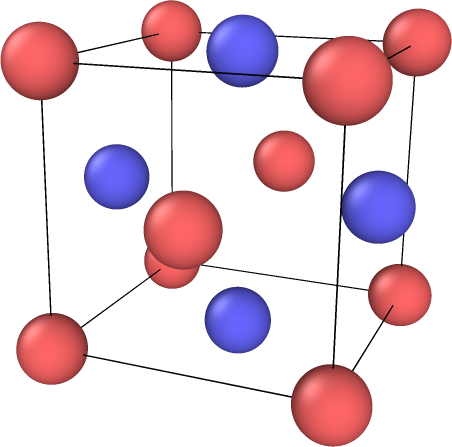
\includegraphics[width=0.07\textwidth]{figures/SoluteCluster_111122.png}\\%
$E^{4Cu}_{Unrelaxed}$(eV)&0.322& $-$ &0.435&0.464&\emph{0.576 / 0.093}&  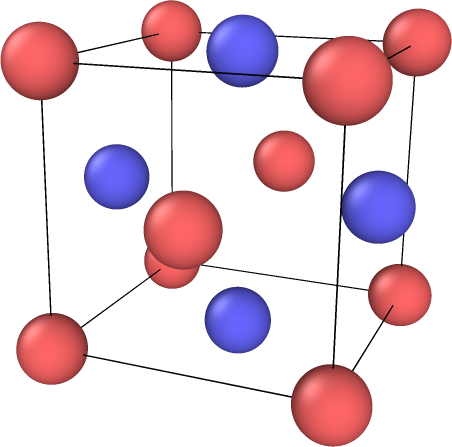
\includegraphics[width=0.07\textwidth]{figures/SoluteCluster_111122.png}\\%
$E^{10Cu}_{Unrelaxed}$(eV)&1.62& $-$ &1.589& 2.254 &\emph{2.275 / 0.618}&  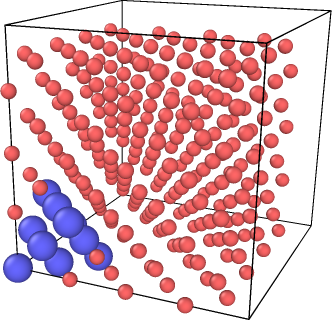
\includegraphics[width=0.07\textwidth]{figures/SoluteCluster_10atoms.png}\\%
%$E^{10Cu}_{Unrelaxed}$(eV)&1.62& $-$ &\textcolor{red}{?}& - &\emph{ / }&  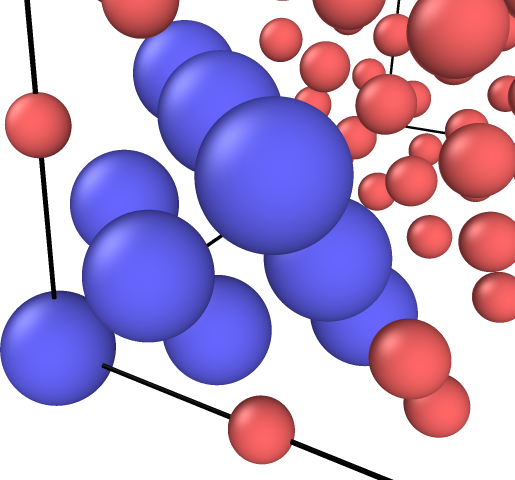
\includegraphics[width=0.07\textwidth]{figures/SoluteCluster_10atoms_v2.png}\\%
\hline%
\end{tabular}%
\caption{Cu cluster energies for DFT, ADP and NNP. Clusters are described using the the length of edges of the cluster, e.g., 111 represents three edges all nearest neighbors. Note that there are three edges for a three atom cluster but six edges for a four atom cluster.
}
\label{table:solute_cluster}
\end{table}


\begin{table}[H]
	\centering
	\begin{tabular}{l|ccccc}
		\toprule
		& \multicolumn{5}{c}{Migration energy [eV]}                   \\
		\cmidrule(r){2-6}
		Rate         & DFT$^1$    & ADP  & NNP11 & NNP10  & NNP-\emph{Avg / StdDev}  \\
		\midrule
		$\omega^{0}$ & 0.58 & 0.63 & 0.58 & 0.58 & \emph{0.58 / 0.01}\\
		$\omega^{1}$ & 0.38 & 0.46 & 0.41 & 0.42 & \emph{0.42 / 0.02}\\
		$\omega^{2}$ & 0.57 & 0.76 & 0.43 & 0.52 & \emph{0.47 / 0.04}\\
		\bottomrule
	\end{tabular}
	\caption{Vacancy migration barriers with a single Cu atom in the Al matrix. The labels (0,1,2) are consistent with the 5-frequency model for FCC lattice. $^1$The reported DFT results were computed by Mantina \textit{et. al}\cite{Mantina2009FirstCoefficients}.}
	\label{tab:vacmig}
\end{table}


To examine the early-stage clustering under realistic conditions of time and temperature, we perform off-lattice KMC simulations of the evolution of an Al-4-5\% Cu alloy starting from a random solid solution state.  For this demonstration, we use the bulk vacancy migration barrier $E^{Mig}_{Al}$ in Al (computed from DFT) as the migration barrier for all vacancy-mediated transitions, and compute the enthalpy barrier between the initial state $i$ and final state $f$ using a simple chemical-kinetics model as
\begin{equation}
E^{Mig}_{i-f}= E^{Mig}_{Al} + (E_{f} - E_{i})/2
\end{equation}
Where $E_{f}$ and $E_{i}$ are the fully-relaxed final and initial state energies of the entire system.  Table ~\ref{tab:vacmig} shows the migration barriers for the three main transitions [DO NOT USE $\omega$ NOTATION - EITHER USE WORDS OR ADD A SMALL FIGURE AS IN TABLE 4 PICTURES.  WORDS SHOULD BE FINE - E.G. BULK V-AL EXCHANGE , V-CU EXCHANGE, AND V-AL EXCHANGE IN V-AL-CU TRIPLET OR SOMETHING....]  in the 5-frequency model as computed via DFT\cite{Mantina2009FirstCoefficients}, NNP11, and also NNP10 that will be discussed further below.  All three migration barriers are well-captured by both NNPs but the approximation above will use only $\omega_0$ for all transitions, including those in and around small clusters the form during the KMC.  Thus, the KMC will satisfy detailed balance and capture the correct thermodynamics but not represent the true time-scale of evolution\cite{Mantina2009FirstCoefficients} of the system. We use a 1000 atom supercell containing one vacancy and execute simulations at 300K with 4\% Cu and at 696K with 5\% Cu using both NNP11 and NNP10, the latter providing a better representation of the energetics of the 3- and 4- atom Cu clusters shown in Table \ref{table:solute_cluster}.

Figure~\ref{fig:gp1} shows KMC simulations using NNP11 and NNP10 with Al-4\% Cu at 300K after $5\times10^{5}$ KMC steps.  Both systems ultimately form Cu GP-I precipitates consistent with real alloys under similar conditions. NNP11 requires a much longer time, nearly 1 sec, before the GP-I starts to form as compared to NNP10 (less than 0.1 sec), which may reflect the different competing energetics of the various 3- and 4-atom clusters in NNP11 as compared to NNP10. The NNP10 structure also has a much lower energy, indicating a more-well-formed precipitation state, relative to NNP11, again indicating that the GP-I formation with NNP11 may compete energetically with some other structures at the early stages of formation. Starting the KMC simulation from different initial random geometries and/or other NNPs leads to the formation of GP-I within a similar time-frame and energy levels. The NNPs thus consistently capture the behavior expected in real materials.  Gorbatov et al. and Ogata et al. have recently presented KMC studies of the same problem, showing similar formation of the GP-I zones, and so our results are not unique.  However, Gorbatov et al. used a cluster expansion method that, while suitable for KMC, cannot be used for any other studies beyond Al-Cu thermodynamics such as plasticity and fracture studies.  Ogata et al. used a new EAM-type Al-Cu potential, and such a potential would require significant more validation across many properties shown here before it could be deemed broadly applicable to the Al-Cu system.  The NNPs show the expected precipitation behavior while also being valid for a wide range of applications.

KMC simulations at higher temperature (696K) (and slightly higher Cu concentration (5\%)) reveal pitfalls of some of the NNPs, however.  For a few NNPs (NNP 13, XX, YY, ZZ), a dense block of FCC Cu is formed with a very low energy compared to the initial solid solution.  This spurious behavior arises because these NNPs have negative formation energies for the 3-atom 111 and 4-atom tetrahedral 111111 clusters (table~\ref{table:solute_cluster}) and even larger formation energies for larger dense clusters (10 atom cluster shown in table~\ref{table:solute_cluster}.  This incorrect feature favors nucleation and then growth of the dense FCC Cu.  Neither NNP11 nor NNP10 has this error, and so KMC simulations at 696K show no precipitation and only sporadic few-atom clusters of Cu; this is consistent with expectations for real Al-Cu under these conditions.  

The above findings reinforce that careful validation of any potential (NNP or otherwise) must be done within the range of structures for which the NNP will be used.  This result also highlights the use of multiple NNPs for the same problem, especially extracting new structures from a simulation using NNP-X and evaluating them using other NNPs.  Finally, having a family of NNPs can enable mixing and matching of the NNPs in a set of related studies - e.g. NNP10 being used for precipitate evolution in KMC, for instance, while NNP11 (or some other choice) being employed to study dislocations moving through the microstructure established using NNP10.  The close agreement among the family of NNPs for many properties makes such a mix-and-match strategy feasible in a manner that is not as feasible using traditional potentials.


\begin{figure}[H]
  \centering
  \includegraphics[width=6.5in]{kmcFigures/gp1.pdf}
  \caption{Energy vs simulation time and the final geometry showing Cu GP1 precipitate formation. The simulations were carried out with potential number '10' and '11' at 300K using a 1000 atom supercell containing 40 Cu atoms for $5\times10^6$ KMC steps.
  }
  \label{fig:gp1}
\end{figure}
%
%\begin{figure}[H]
%  \centering
%  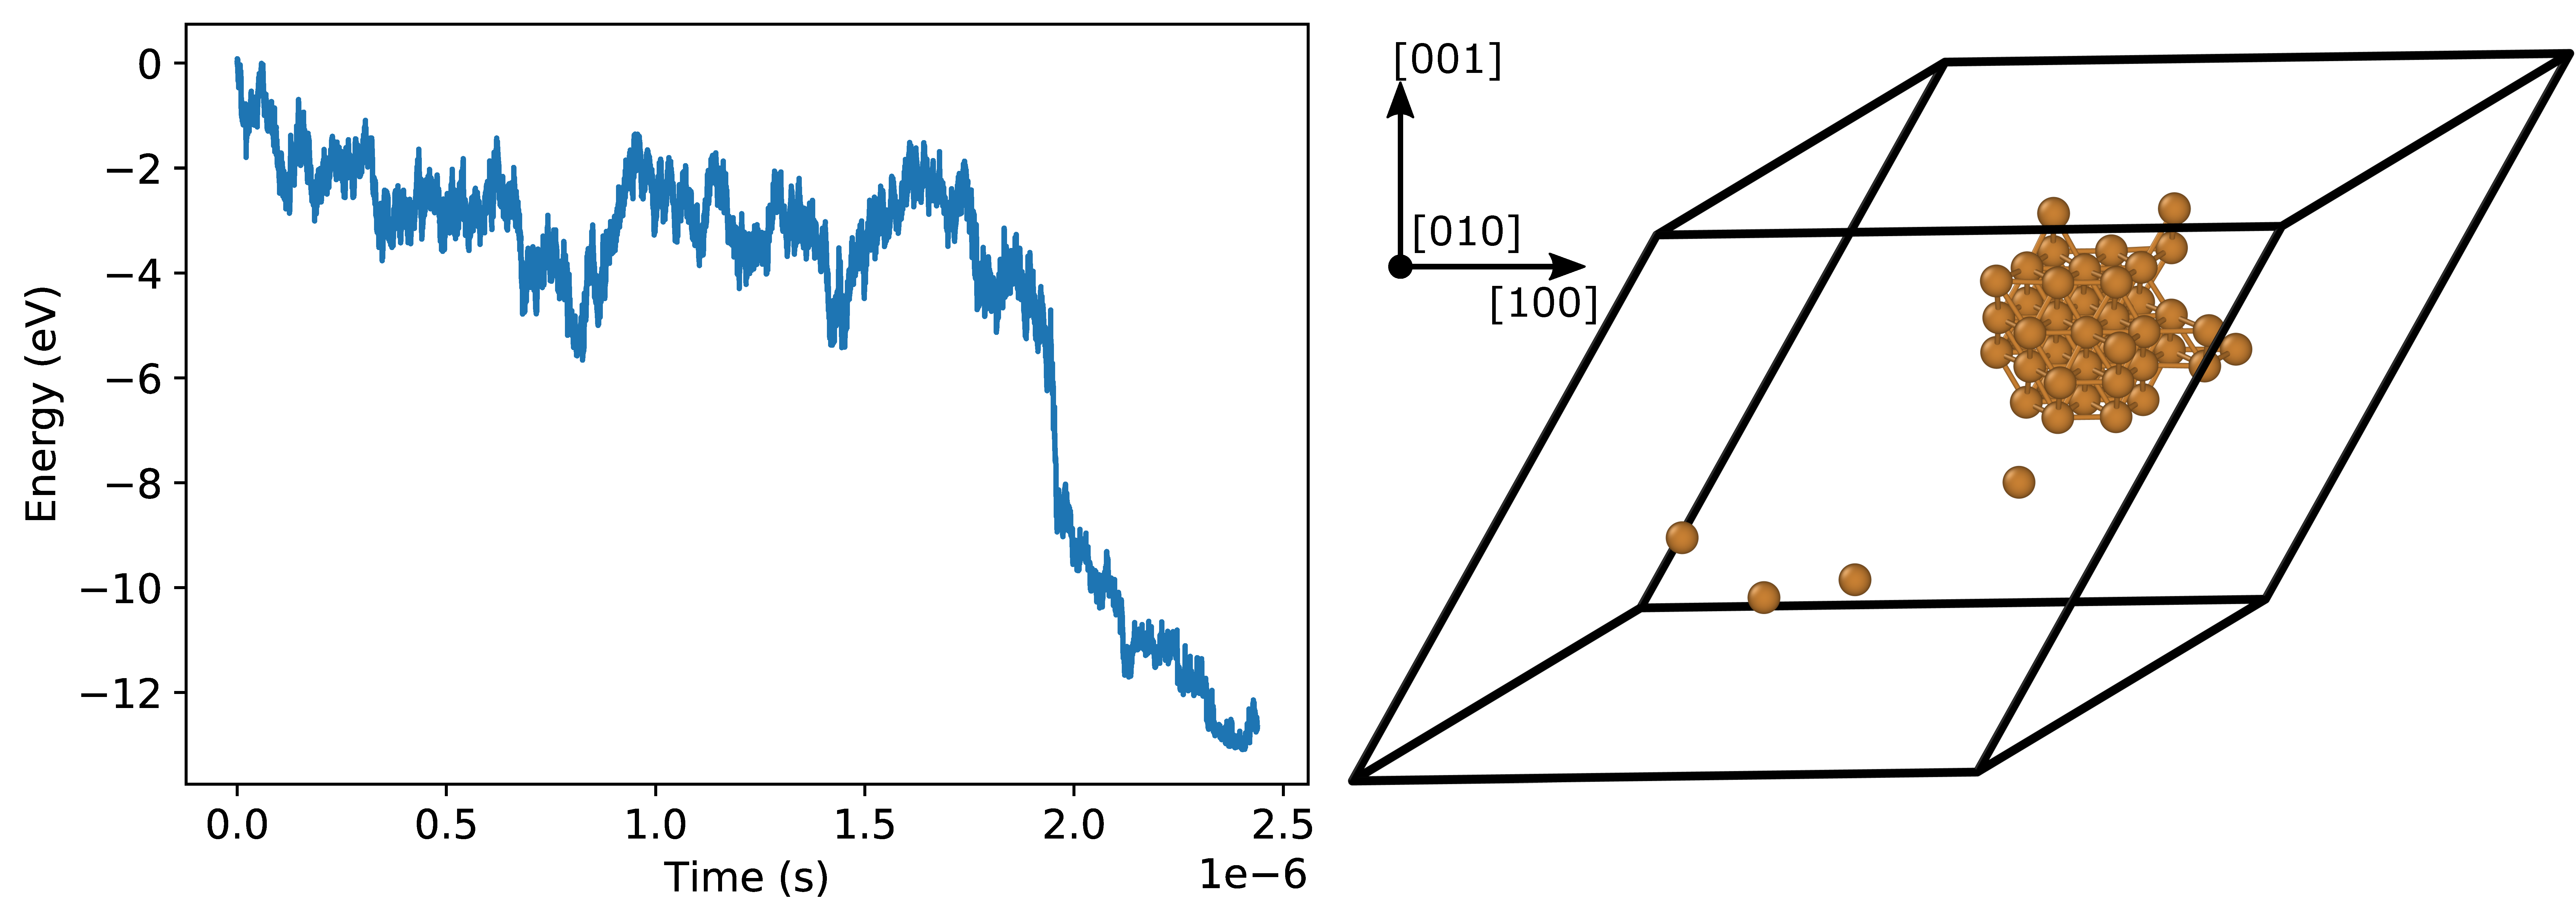
\includegraphics[width=6.5in]{kmcFigures/cubulk.pdf}
%  \caption{Energy vs simulation time and the final geometry showing the non-physical Cu precipitate. The simulation was carried out with potential number '13' at 696K using a 1000 atom supercell containing 50 Cu atoms for $5\times10^6$ KMC steps.
%  \textcolor{red}{Likely to change this figure to a run with the with best C44 potential}
%  }
%  \label{fig:cubulk}
%\end{figure}

\subsection{Dislocations and Fracture in Aluminum} \label{sct:fracture_dislocation}

In any applications of potentials to plasticity and fracture, it is essential to demonstrate that the potential reproduces a reasonable structure for the relevant dislocation(s) and exhibits physically-expected behavior at sharp crack tips.  There are no precise first-principles results for comparisons, but DFT results using other settings and novel simulations methods provide a approximate references for determining whether the ML potential is reasonable and physical.  An ML potential can also be compared to other traditional potentials where the behavior has previously been found reasonable.

With that background, we examined the predictions of the NNP11 potential for the structure and energetics of the $a$<110>/2 edge and screw dislocations in pure Al.
The methodology to create the dislocation is standard, and described in \cite{Hu2020AtomisticDynamics}.
An edge or screw dislocation is placed at the center of a cylindrical cell of radius 31.48 ($\AA$) RECHECK WITH YI - THIS RADIUS IS SMALL AND THE BOUNDARY REGION OF 22 A LEAVES NO SPACE FOR THE DISLOCATION, PRACTICALLY - ONE OR THE OTHER IS NOT CORRECT.
All atoms in the cell are deformed according to the anisotropic displacement field of a Volterra dislocation computed using the Stroh formalism\cite{Stroh1958DislocationsElasticity}.
Atoms within 22$\AA$ of the outer boundary are then fixed at these initial positions, and all interior atoms relaxed to a minimum energy condition.
The core structure for both edge and screw dislocations for NNP11 is shown in Figure \ref{fig:dislocation_NNPvsDFT} along with the DFT-computed structure from \cite{Woodward2008PredictionTheory}.
The NNP11 dislocation dissociates into two partial dislocations, as expected.
The dissociation distance between the two partials differs slightly from the DFT reference, recalling that the NNP11 has a higher $C_{44}$ then usually obtained in DFT and that this DFT structure is obtained by very different methodology and DFT parameters.

\begin{figure}[H]%
\centering%
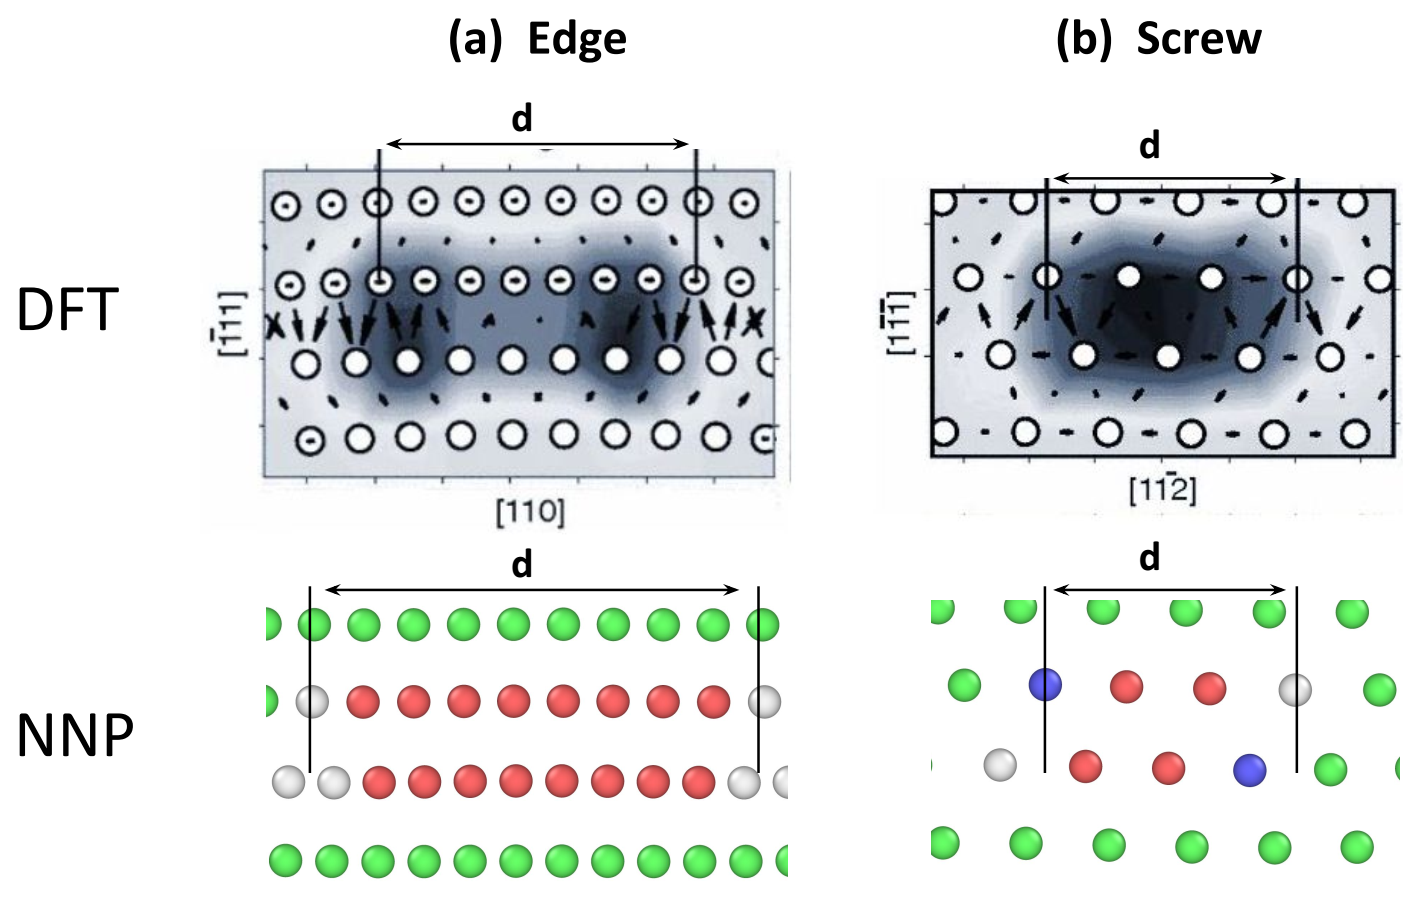
\includegraphics[width=1\textwidth,center]{figures/dislocation_NNPvsDFT.png}%
\caption{Atomistic structures of the edge and screw $a$<110>/2 dislocations in pure Al as predicted by DFT and NNP11. (a) Edge dislocation: DFT shows the differential displacement map and the estimated partial dislocation spacing; NNP shows atoms identified by common neighbor analysis (green = FCC, red = HCP; white = other) where the HCP atoms lie in the stacking fault between the two partials and the partial core regions appear as white, with the estimated partial dislocation spacing shown. (b) Screw dislocation: as in (a) but where white and blue atoms identify the screw partial cores.
DFT image adapted from \cite{Woodward2008PredictionTheory} with permission of the APS
}%
\label{fig:dislocation_NNPvsDFT}
\end{figure}

As a quantitative measure, we compute the core energy $\Gamma^{core}$ energy of the dislocation as defined at distance $r_c = b$ using the analysis of Ref. \cite{Hu2020AtomisticDynamics}.
We compute $E^{core}=1.144$ eV/nm for the edge dislocation and $1.055$ eV/nm for the screw dislocation, respectively, which compare well to the values from EAM potentials of Ercolessi-Adams\cite{Ercolesi1994InteratomicMethod} (edge: 0.463 eV/nm; screw: 0.810 eV/nm) and Mishin\cite{Mishin1999InteratomicCalculations} (edge: 1.198 eV/nm; screw 1.262 eV/nm) \cite{Hu2020AtomisticDynamics}.  The EAM potentials have been widely used for modeling of dislocations in Al, and so the values obtained for the NNP, along with the accurate structures, indicate the suitability of the NNP for studying dislocations.

Our broad experience with both ML and traditional potentials has indicated that they can struggle to correctly capture behavior at the tip of a sharp crack. 
So here we examine the most basic fracture test for an FCC metals, the emission of a dislocation from a sharp crack tip.
Theoretical models predict that the critical stress intensity factor $K_{Ie}$ for emission of the first partial dislocation from the tip of a crack with crack plane (111) and crack line direction (110) is
\begin{equation}
K_{Ie} =
\begin{cases}
\sqrt{\gamma^{USF}o(\theta^{slip},\phi^{Burgers})}/F_{12}(\theta) & \gamma^{111} \leq 3.45\gamma^{USF}\\
 \sqrt{(0.5\gamma^{USF}+0.145\gamma^{111})o(\theta^{slip},\phi^{Burgers})}/F_{12}(\theta) & \gamma^{111} > 3.45\gamma^{USF}
\end{cases}
\end{equation}
Where $\gamma^{USF}$ is the unstable stacking fault energy, $\gamma^{111}$  is the surface energy of the emission plane, $o(\theta^{slip},\phi^{Burgers})$ is an anisotropic elasticity term dependent on the inclination of the slip plane and Burgers vector, and $F_{12}(\theta^{slip})$ provides the resolved slip on the slip plane oriented at an angle with respect to the crack plane (see Andric \& Curtin\cite{Andric2019AtomisticFracture}).  Using the DFT-computed values of the various material quantities, the critical value is predicted to be $K_{Ie}=0.341$ MPa $\sqrt{\text{m}}$.  A multiscale DFT simulation using the same crack orientation but different DFT parameters\cite{Nair2011} was shown to emit a dislocation at $K_{Ie}$=0.368 (MPa$\sqrt{\text{m}}$).  We note further that emission occurs rather than cleavage because the stress intensity for cleavage, related to the surface energy, is larger than $K_{Ie}$.  This background provides a basis for assessing the NNPs and demonstrates the range of values that can emerge from DFT assessments.

We simulate the crack tip behavior following the K-test methodology carefully described by Andric \& Curtin \cite{Andric2019AtomisticFracture}.  We use a simulation cell of size 200*200*10 $\AA^3$, insert a crack terminating along the $z$ direction in the center of the cell, hold boundary atoms fixed at the anistropic elastic predictions for the desired applied stress intensity factor, and allow all interior atoms to relax using the conjugate-gradient method followed by steepest descent with force tolerance 1$e$-05 ev/A.  Successive increments in load level are applied until any notable event occurs at the crack tip.
All 40 NNPs show partial dislocation emission and with no gross artifacts at the crack tip; a typical example is shown in Figure \ref{fig:fracturedislocation_images}, which is qualitatively similar to results found with many traditional potentials.  The emission event occurs at a critical load of $K_{Ie}=0.354+/-0.007$ (MPa$\sqrt{\text{m}}$) across all 40 NNPs, in very good agreement with the DFT-predicted theoretical value and consistent with the value found in the direct multiscale DFT simulation.  Some variation does arise among the NNPs: 13 NNPs showed emission of only the leading partial (Figure \ref{fig:fracturedislocation_images} (a)) while 27 NNPs showed the emission of a second twinning partial just behind the crack tip (Figure \ref{fig:fracturedislocation_images} (b) following the leading partial with no increase in the applied load.  The NNP simulations are thus consistent with theory and other simulations showing that this second partial emission event is the next expected event.  The load for this second event depends on several additional factors including the unstable twinning fault energy, and results from EAM Al potentials show that the load is only slightly higher than that required for the first event.  The NNP behavior is thus within the scope of reasonable behavior.  Overall, the NNPs for pure Al provide a very good representation of the crack tip and the first partial emission process as compared to DFT, theory, and other simulations.


\section{Conclusion}

We have developed a family of Behler-Parinello-type neural-network potentials (NNPs) for the Al-Cu system based on a comprehensive metallurgically-relevant training dataset based on first-principles DFT.  We have demonstrated the ability of these potentials to predict many different properties of importance in metallurgy, including the many possible phases, solute properties, shearing of precipitates, early stage clustering during annealing, dislocation structures, and crack tip performance.  We emphasize that it is essential to study the performance of any potential across such a broad spectrum of structures if the potential is to be used for realistic studies of atomistic phenomena.  Our examination of the NNPs has included properties that are directly derived from the training dataset, and hence expected to be well-captured by the non-linear regression of the NN method.  But, moreover, we investigated a number of properties and structures that were intentionally not in the training dataset.  The methodology is easily extendable to the inclusion of more training data when the current family of NNPs is found to be inaccurate for some problems, as will undoubtedly be the case in the future.  To facilitate such future advances, our entire DFT training set is available along with the DFT provenance necessary to expand the database using the same DFT parameters.

The NNPs developed here have been extensively compared to the newest and widely-used traditional interatomic potential for Al-Cu, the Angularly-Dependent Potential from Apostol and Mishin.  While the ADP is based on some underlying physical principles, it has far fewer fitting parameters and hence performs comparably to the NNPs only for those few properties to which the ADP is fit.  Across the much broader range of properties that are necessary for realistic metallurgical studies, the NNPs here are demonstrably far better, and the ADP gives unphysical behavior for some important situations.  We reiterate that our purpose is not to denigrate the ADP in particular but rather to show that one of the best traditional alloy potentials has many deficiencies and that a machine learning approach overcomes those deficiencies.  The overarching philosophical concern about the use of ML potentials is that they contain no physics and so can possibly fail very badly in situations where a traditional potential might also fail quantitatively but not qualitatively.  With our comparison of the NNP to ADP, this concern can be partially relieved.  Across a much wider spectrum of properties that must be well-represented for realistic atomic-scale studies in alloys, the NNPs perform far better than the ADP and so it is, in fact, use of the ADP that will more likely introduce hidden errors across a wide scope of possible applications, leading to incorrect predictions either qualitatively or quantitatively.  A compromise strategy, emerging in the literature, is to combine a traditional potential such as the ADP with an ML potential that is trained on the difference between the traditional potential and a DFT training set.  Such a strategy can be pursued in the future for Al-Cu using our openly-available DFT training set.

The family of NNPs is not perfect.  Most notably, $C_{44}$ of Al has substantial errors even with careful inclusion of relevant structures.
Across our family of NNPs, and adding structures intended to bias the optimization toward a better representation of $C_{44}$, we could not achieve an error below 10\%.  Similarly, we could not reduce the errors on solute pair energies below ~20meV, again despite the careful inclusion of structures in the training set.  These limitations might be resolved through the use of other ML methods, other optimization methods based on energy differences between structures rather than absolute energies, a larger set of descriptors for the atomic environments, etc., and all of these can also be pursued in the future using our openly-available DFT training set.

In summary, we have demonstrated that a machine learning interatomic potential can be created that accurately captures the exceptionally rich and diverse phase space of a binary alloy, here Al-Cu, with very good and physical performance for material properties and structural response that are necessary for metallurgical studies.  This demonstration points to continued development of ML-based interatomic potentials based on an extensive database of carefully-chosen metallurgically-relevant structures as a viable path toward the quantitative study of metal alloys at the atomic scale.

\section{Acknowledgements}
The authors acknowledge support for this work by the NCCR MARVEL, funded by the Swiss National Science Foundation. The authors would also like to acknowledge E. Mak for running the fracture simulations, Y. Hu for the dislocation results, Dr. B. Yin for helpful discussions regarding DFT calculations, R. Ahmad for insight into GSF structures, and Drs. G. Pizzi \& S. Huber for their help in running AiiDA.

\newpage
\bibliographystyle{unsrt}  
\bibliography{references}  %%% Remove comment to use the external .bib file (using bibtex).
%%% and comment out the ``thebibliography'' section.

\newpage
\appendix
\section{Supplementary}
\subsection{Symmetry Function Hyperparameters} \label{apd_sct:symmfunc_hyperparam}

\bgroup
\def\arraystretch{1.2}
\begin{longtable}{ccccc}
\caption{Hyperparameters for the radial symmetry functions.} \\
\hline
Element1 & Element2 & $\eta$ & $r_2$ & $r_c$ \\
\hline
\hline
Al &  Al & $1.117 \times 10^{-1}$ & $1.301 \times 10^{1}$ & $1.600 \times 10^{1}$ \\
Al &  Al & $1.166 \times 10^{-1}$ & $7.071 \times 10^{0}$ & $2.000 \times 10^{1}$ \\
Al &  Al & $1.350 \times 10^{-1}$ & $9.170 \times 10^{0}$ & $2.000 \times 10^{1}$ \\
Al &  Al & $1.560 \times 10^{-2}$ & $0.000 \times 10^{0}$ & $8.000 \times 10^{0}$ \\
Al &  Al & $1.689 \times 10^{-1}$ & $1.057 \times 10^{1}$ & $1.600 \times 10^{1}$ \\
Al &  Al & $2.109 \times 10^{-1}$ & $7.336 \times 10^{0}$ & $1.600 \times 10^{1}$ \\
Al &  Al & $2.500 \times 10^{-3}$ & $0.000 \times 10^{0}$ & $2.000 \times 10^{1}$ \\
Al &  Al & $2.982 \times 10^{-1}$ & $6.169 \times 10^{0}$ & $8.000 \times 10^{0}$ \\
Al &  Al & $3.900 \times 10^{-3}$ & $0.000 \times 10^{0}$ & $1.600 \times 10^{1}$ \\
Al &  Al & $4.466 \times 10^{-1}$ & $6.504 \times 10^{0}$ & $8.000 \times 10^{0}$ \\
Al &  Al & $4.770 \times 10^{-2}$ & $1.542 \times 10^{1}$ & $2.000 \times 10^{1}$ \\
Al &  Al & $5.830 \times 10^{-2}$ & $1.000 \times 10^{1}$ & $2.000 \times 10^{1}$ \\
Al &  Al & $6.900 \times 10^{-3}$ & $0.000 \times 10^{0}$ & $1.200 \times 10^{1}$ \\
Al &  Al & $7.100 \times 10^{-3}$ & $0.000 \times 10^{0}$ & $2.000 \times 10^{1}$ \\
Al &  Al & $7.430 \times 10^{-2}$ & $0.000 \times 10^{0}$ & $8.000 \times 10^{0}$ \\
Al &  Al & $8.020 \times 10^{-2}$ & $1.189 \times 10^{1}$ & $2.000 \times 10^{1}$ \\
Al &  Cu & $1.117 \times 10^{-1}$ & $1.301 \times 10^{1}$ & $1.600 \times 10^{1}$ \\
Al &  Cu & $1.166 \times 10^{-1}$ & $7.071 \times 10^{0}$ & $2.000 \times 10^{1}$ \\
Al &  Cu & $1.350 \times 10^{-1}$ & $9.170 \times 10^{0}$ & $2.000 \times 10^{1}$ \\
Al &  Cu & $1.689 \times 10^{-1}$ & $1.057 \times 10^{1}$ & $1.600 \times 10^{1}$ \\
Al &  Cu & $2.109 \times 10^{-1}$ & $7.336 \times 10^{0}$ & $1.600 \times 10^{1}$ \\
Al &  Cu & $2.500 \times 10^{-3}$ & $0.000 \times 10^{0}$ & $2.000 \times 10^{1}$ \\
Al &  Cu & $2.982 \times 10^{-1}$ & $6.169 \times 10^{0}$ & $8.000 \times 10^{0}$ \\
Al &  Cu & $4.466 \times 10^{-1}$ & $6.504 \times 10^{0}$ & $8.000 \times 10^{0}$ \\
Al &  Cu & $4.770 \times 10^{-2}$ & $1.542 \times 10^{1}$ & $2.000 \times 10^{1}$ \\
Al &  Cu & $5.830 \times 10^{-2}$ & $1.000 \times 10^{1}$ & $2.000 \times 10^{1}$ \\
Al &  Cu & $6.900 \times 10^{-3}$ & $0.000 \times 10^{0}$ & $1.200 \times 10^{1}$ \\
Al &  Cu & $7.100 \times 10^{-3}$ & $0.000 \times 10^{0}$ & $2.000 \times 10^{1}$ \\
Al &  Cu & $8.020 \times 10^{-2}$ & $1.189 \times 10^{1}$ & $2.000 \times 10^{1}$ \\
Al &  Cu & $9.510 \times 10^{-2}$ & $0.000 \times 10^{0}$ & $2.000 \times 10^{1}$ \\
Cu &  Al & $1.000 \times 10^{-2}$ & $0.000 \times 10^{0}$ & $2.000 \times 10^{1}$ \\
Cu &  Al & $1.073 \times 10^{-1}$ & $0.000 \times 10^{0}$ & $1.600 \times 10^{1}$ \\
Cu &  Al & $1.117 \times 10^{-1}$ & $1.301 \times 10^{1}$ & $1.600 \times 10^{1}$ \\
Cu &  Al & $1.166 \times 10^{-1}$ & $7.071 \times 10^{0}$ & $2.000 \times 10^{1}$ \\
Cu &  Al & $1.350 \times 10^{-1}$ & $9.170 \times 10^{0}$ & $2.000 \times 10^{1}$ \\
Cu &  Al & $1.689 \times 10^{-1}$ & $1.057 \times 10^{1}$ & $1.600 \times 10^{1}$ \\
Cu &  Al & $2.109 \times 10^{-1}$ & $7.336 \times 10^{0}$ & $1.600 \times 10^{1}$ \\
Cu &  Al & $2.500 \times 10^{-3}$ & $0.000 \times 10^{0}$ & $2.000 \times 10^{1}$ \\
Cu &  Al & $2.982 \times 10^{-1}$ & $6.169 \times 10^{0}$ & $8.000 \times 10^{0}$ \\
Cu &  Al & $3.900 \times 10^{-3}$ & $0.000 \times 10^{0}$ & $1.600 \times 10^{1}$ \\
Cu &  Al & $4.466 \times 10^{-1}$ & $6.504 \times 10^{0}$ & $8.000 \times 10^{0}$ \\
Cu &  Al & $4.770 \times 10^{-2}$ & $1.542 \times 10^{1}$ & $2.000 \times 10^{1}$ \\
Cu &  Al & $5.830 \times 10^{-2}$ & $1.000 \times 10^{1}$ & $2.000 \times 10^{1}$ \\
Cu &  Al & $6.900 \times 10^{-3}$ & $0.000 \times 10^{0}$ & $1.200 \times 10^{1}$ \\
Cu &  Al & $8.020 \times 10^{-2}$ & $1.189 \times 10^{1}$ & $2.000 \times 10^{1}$ \\
Cu &  Cu & $1.000 \times 10^{-2}$ & $0.000 \times 10^{0}$ & $2.000 \times 10^{1}$ \\
Cu &  Cu & $1.117 \times 10^{-1}$ & $1.301 \times 10^{1}$ & $1.600 \times 10^{1}$ \\
Cu &  Cu & $1.166 \times 10^{-1}$ & $7.071 \times 10^{0}$ & $2.000 \times 10^{1}$ \\
Cu &  Cu & $1.350 \times 10^{-1}$ & $9.170 \times 10^{0}$ & $2.000 \times 10^{1}$ \\
Cu &  Cu & $1.560 \times 10^{-2}$ & $0.000 \times 10^{0}$ & $8.000 \times 10^{0}$ \\
Cu &  Cu & $1.600 \times 10^{-1}$ & $0.000 \times 10^{0}$ & $2.000 \times 10^{1}$ \\
Cu &  Cu & $1.689 \times 10^{-1}$ & $1.057 \times 10^{1}$ & $1.600 \times 10^{1}$ \\
Cu &  Cu & $2.109 \times 10^{-1}$ & $7.336 \times 10^{0}$ & $1.600 \times 10^{1}$ \\
Cu &  Cu & $2.500 \times 10^{-3}$ & $0.000 \times 10^{0}$ & $2.000 \times 10^{1}$ \\
Cu &  Cu & $2.982 \times 10^{-1}$ & $6.169 \times 10^{0}$ & $8.000 \times 10^{0}$ \\
Cu &  Cu & $3.900 \times 10^{-3}$ & $0.000 \times 10^{0}$ & $1.600 \times 10^{1}$ \\
Cu &  Cu & $4.466 \times 10^{-1}$ & $6.504 \times 10^{0}$ & $8.000 \times 10^{0}$ \\
Cu &  Cu & $4.770 \times 10^{-2}$ & $1.542 \times 10^{1}$ & $2.000 \times 10^{1}$ \\
Cu &  Cu & $5.830 \times 10^{-2}$ & $1.000 \times 10^{1}$ & $2.000 \times 10^{1}$ \\
Cu &  Cu & $6.900 \times 10^{-3}$ & $0.000 \times 10^{0}$ & $1.200 \times 10^{1}$ \\
Cu &  Cu & $8.020 \times 10^{-2}$ & $1.189 \times 10^{1}$ & $2.000 \times 10^{1}$ \\
\hline
\end{longtable}
\egroup

\begin{table}[H]
\caption{Hyperparameters for the angular symmetry functions.}
\centering
\vspace{1em}
\bgroup
\def\arraystretch{1.2}
\begin{tabular}{cccccccc}
\hline
Element1 & Element2 & Element3 & $\eta$ & $\lambda$ & $\zeta$ & $r_c$\\
\hline
\hline
Al &  Al &  Al & $3.900 \times 10^{-3}$ &  1 &  1.0 & $1.600 \times 10^{1}$ \\
Al &  Al &  Cu & $3.900 \times 10^{-3}$ &  1 &  1.0 & $1.600 \times 10^{1}$ \\
Cu &  Al &  Cu & $3.900 \times 10^{-3}$ &  1 &  1.0 & $1.600 \times 10^{1}$ \\
\hline
\end{tabular}
\label{table:symfunc_angular_hypers}
\egroup
\end{table}

%\subsection{Histogram of Errors} \label{apd_sct:rmse_histogram}
%
%\begin{figure}[H]%
%\centering%
%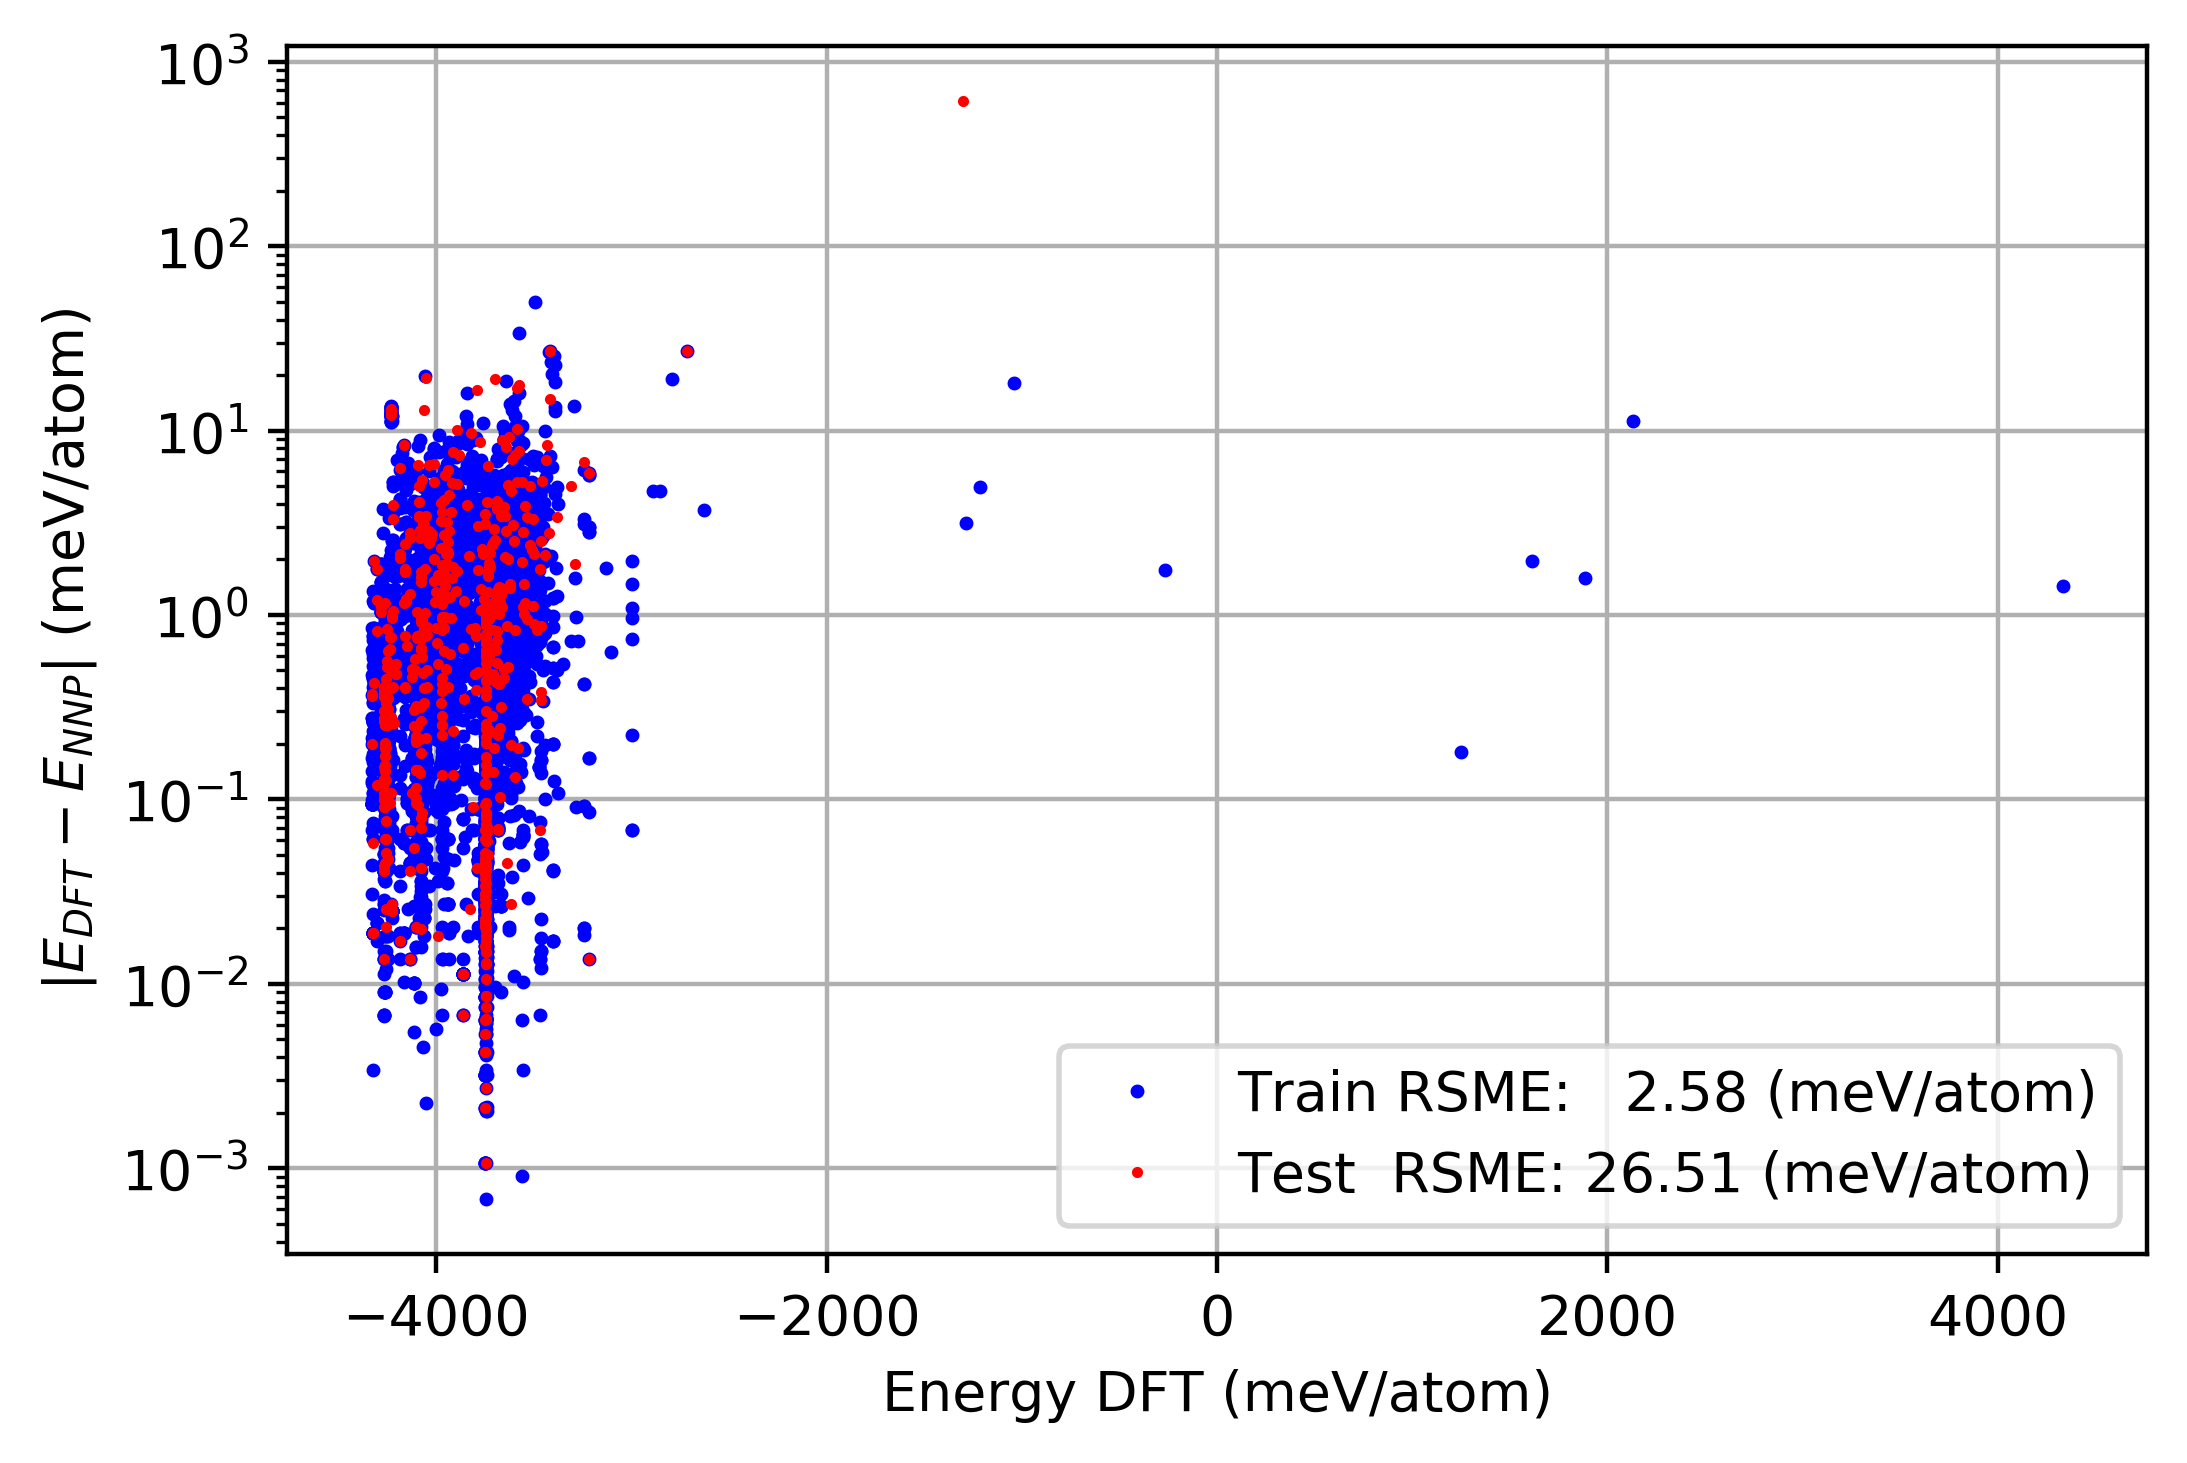
\includegraphics[width=1.0\textwidth,center]{figures/plot_nnperrors.png}%
%\caption{DFT Energy vs Deviation from DF.
%Note the large test error outlier, an order of magnitude larger than the next-greatest test error. }%
%\label{fig:rmse_plot}
%\end{figure}


\subsection{Equation of State of NNP} \label{apd_sct:eos_data}

\begin{figure}[H]%
\centering%
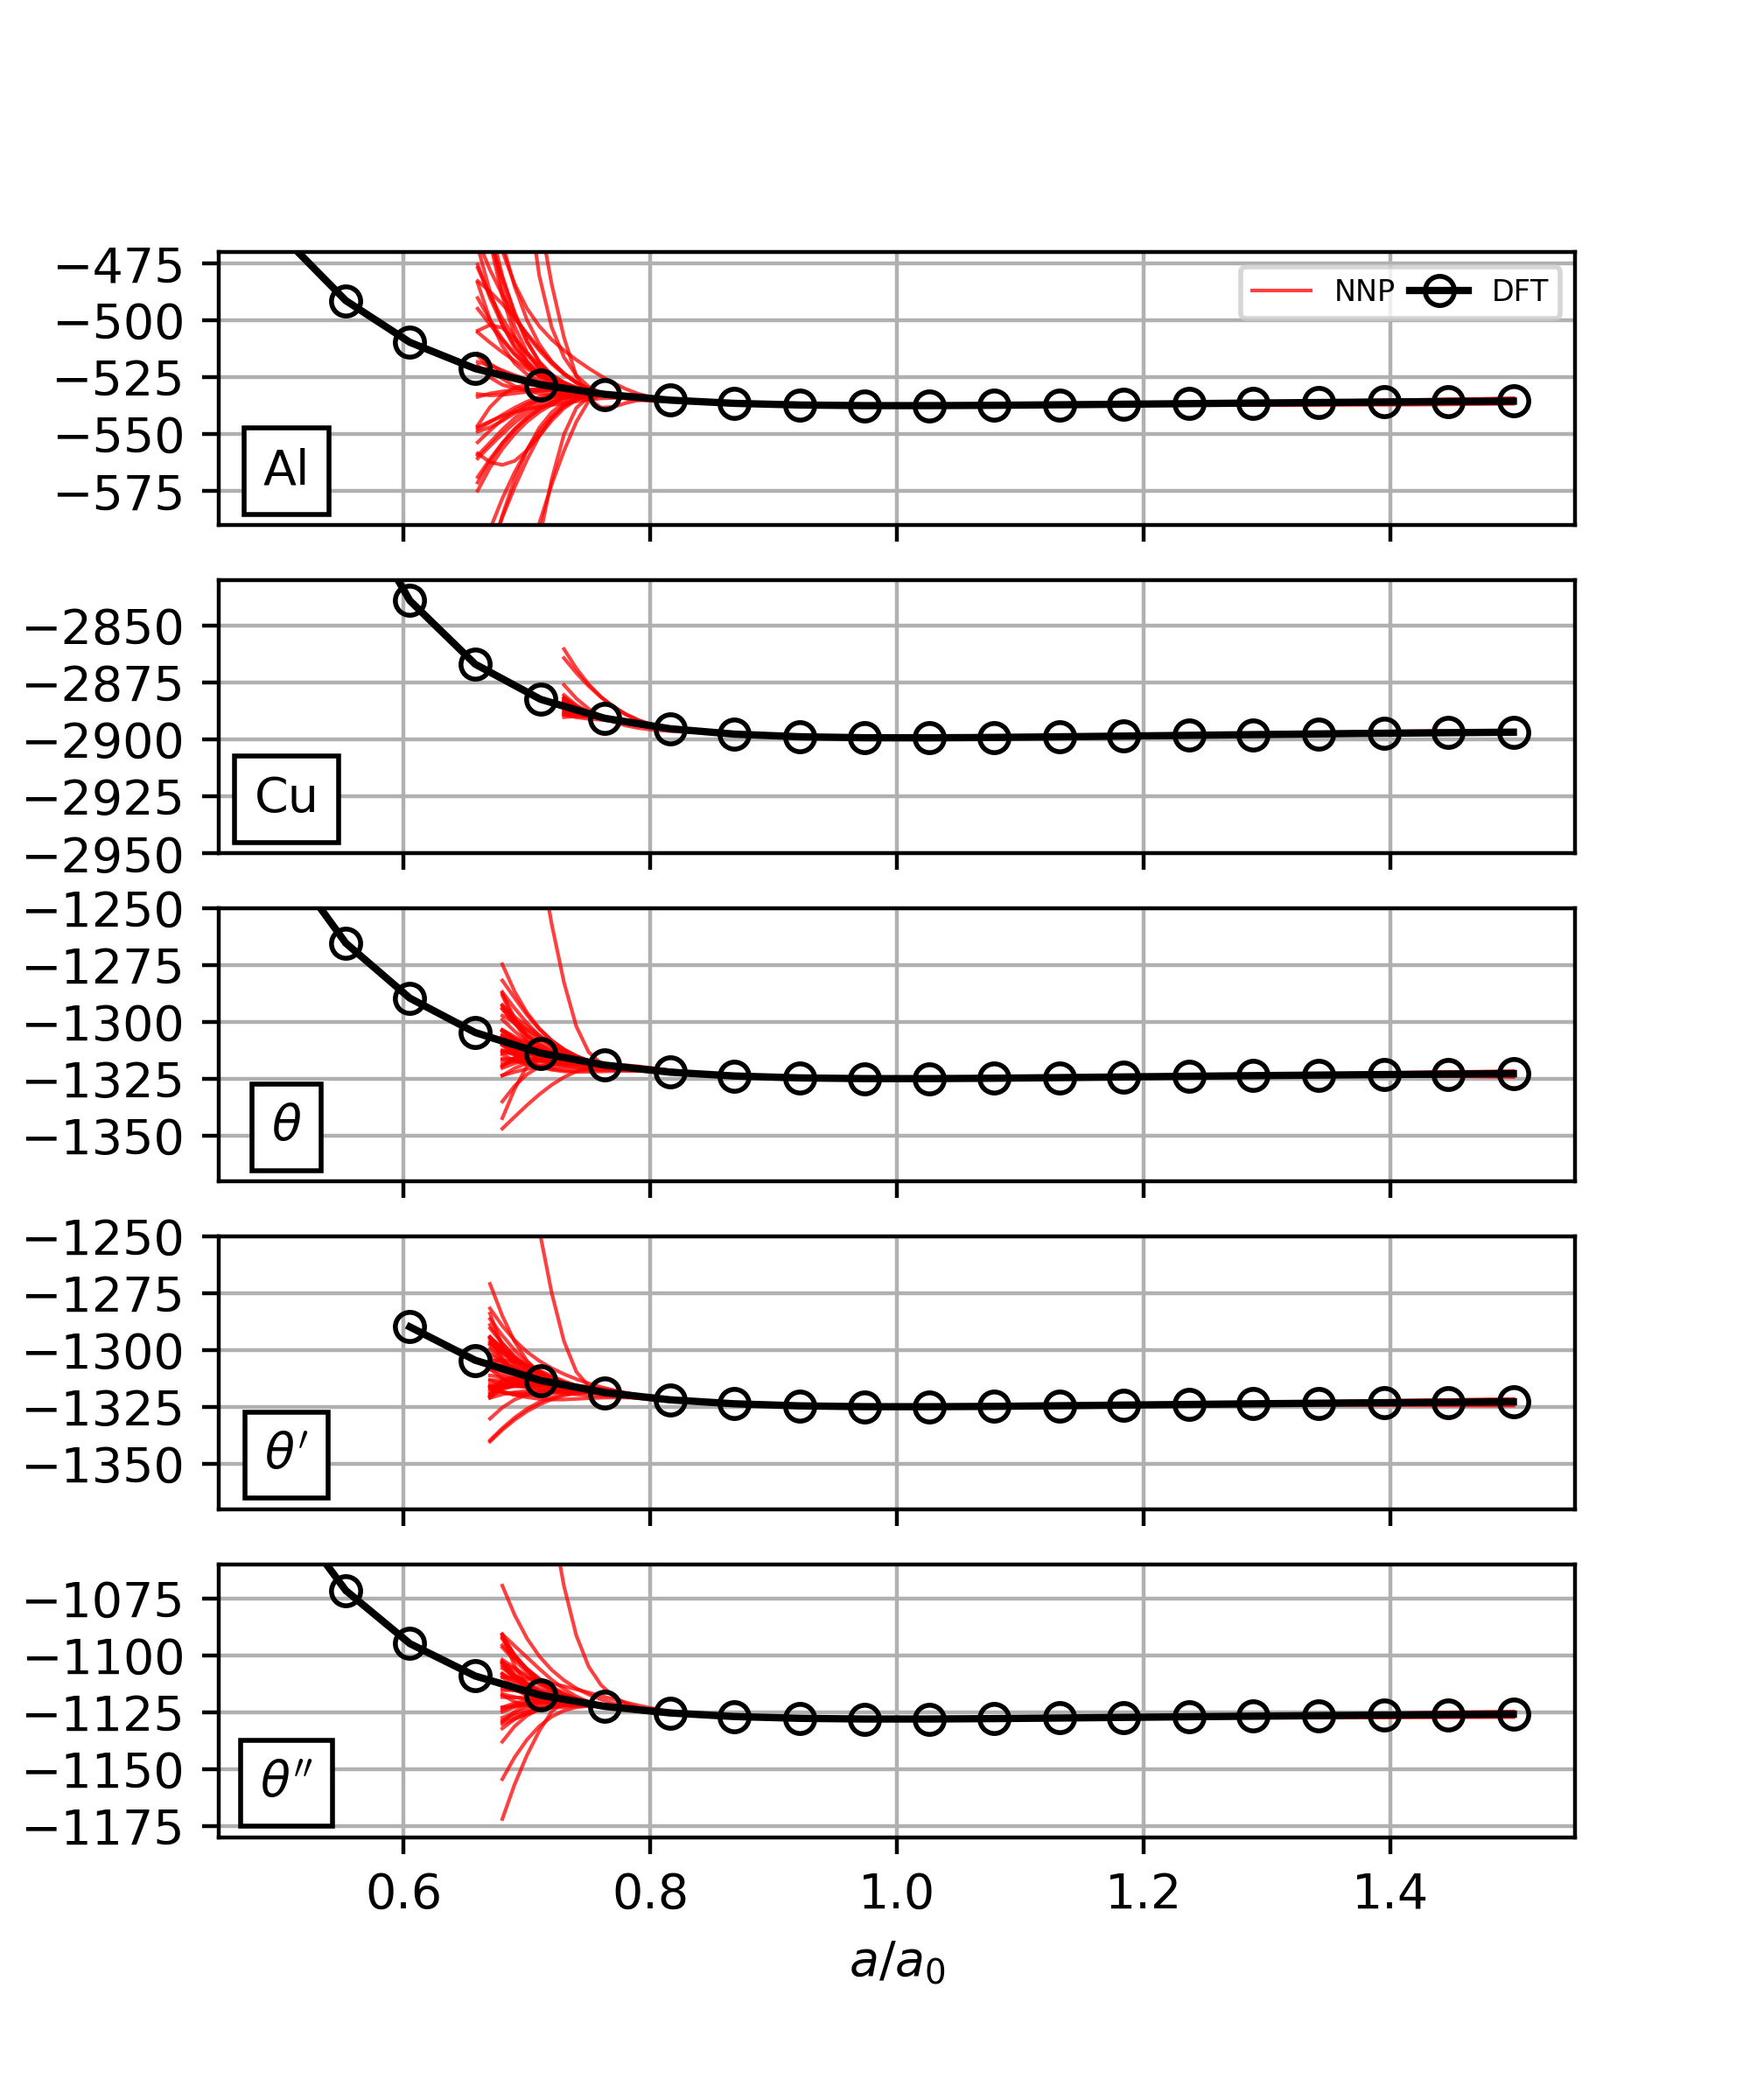
\includegraphics[width=1.0\textwidth,center]{figures/EOS_all.png}%
\caption{Energy vs $a/a_0$ for Al, Cu, $\theta$, $\theta'$, $\theta''$ using NNP and DFT. Only structures with a $a/a_0$ between 1.2 and 0.8 were included in training.}%
\end{figure}


\begin{landscape}
\subsection{Additional Interface Formation Energy Plots} \label{apd_sct:add_interface}

\begin{figure}[H]%
\centering%
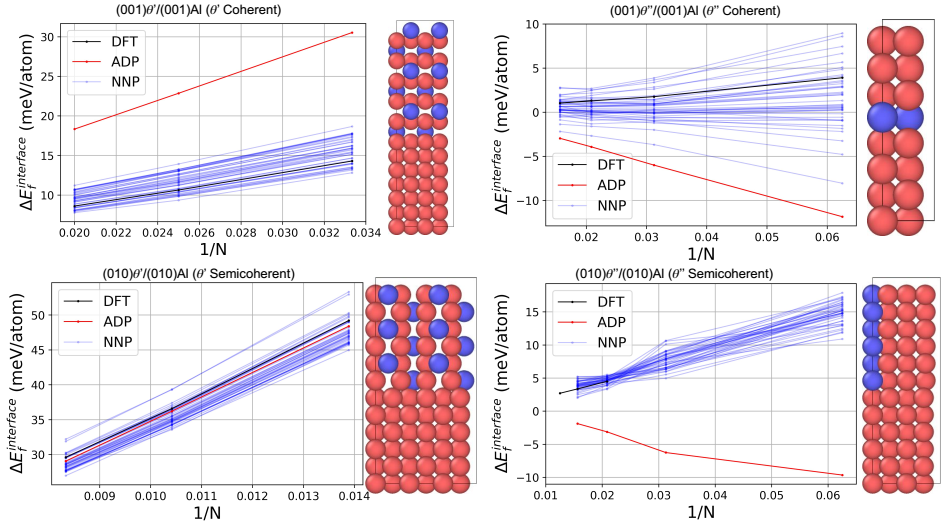
\includegraphics[width=1.4\textwidth,center]{figures/InterfaceAll.png}%
\caption{Interface formation enregy vs inverse number of atoms, with atomic illustration of all interfaces considered in this work}%
\label{fig:interface_structures}
\end{figure}
\end{landscape}


\subsection{Additional Solute Plots and Figures} \label{apd_sct:adn_solsol}

\begin{figure}[H]%
\centering%
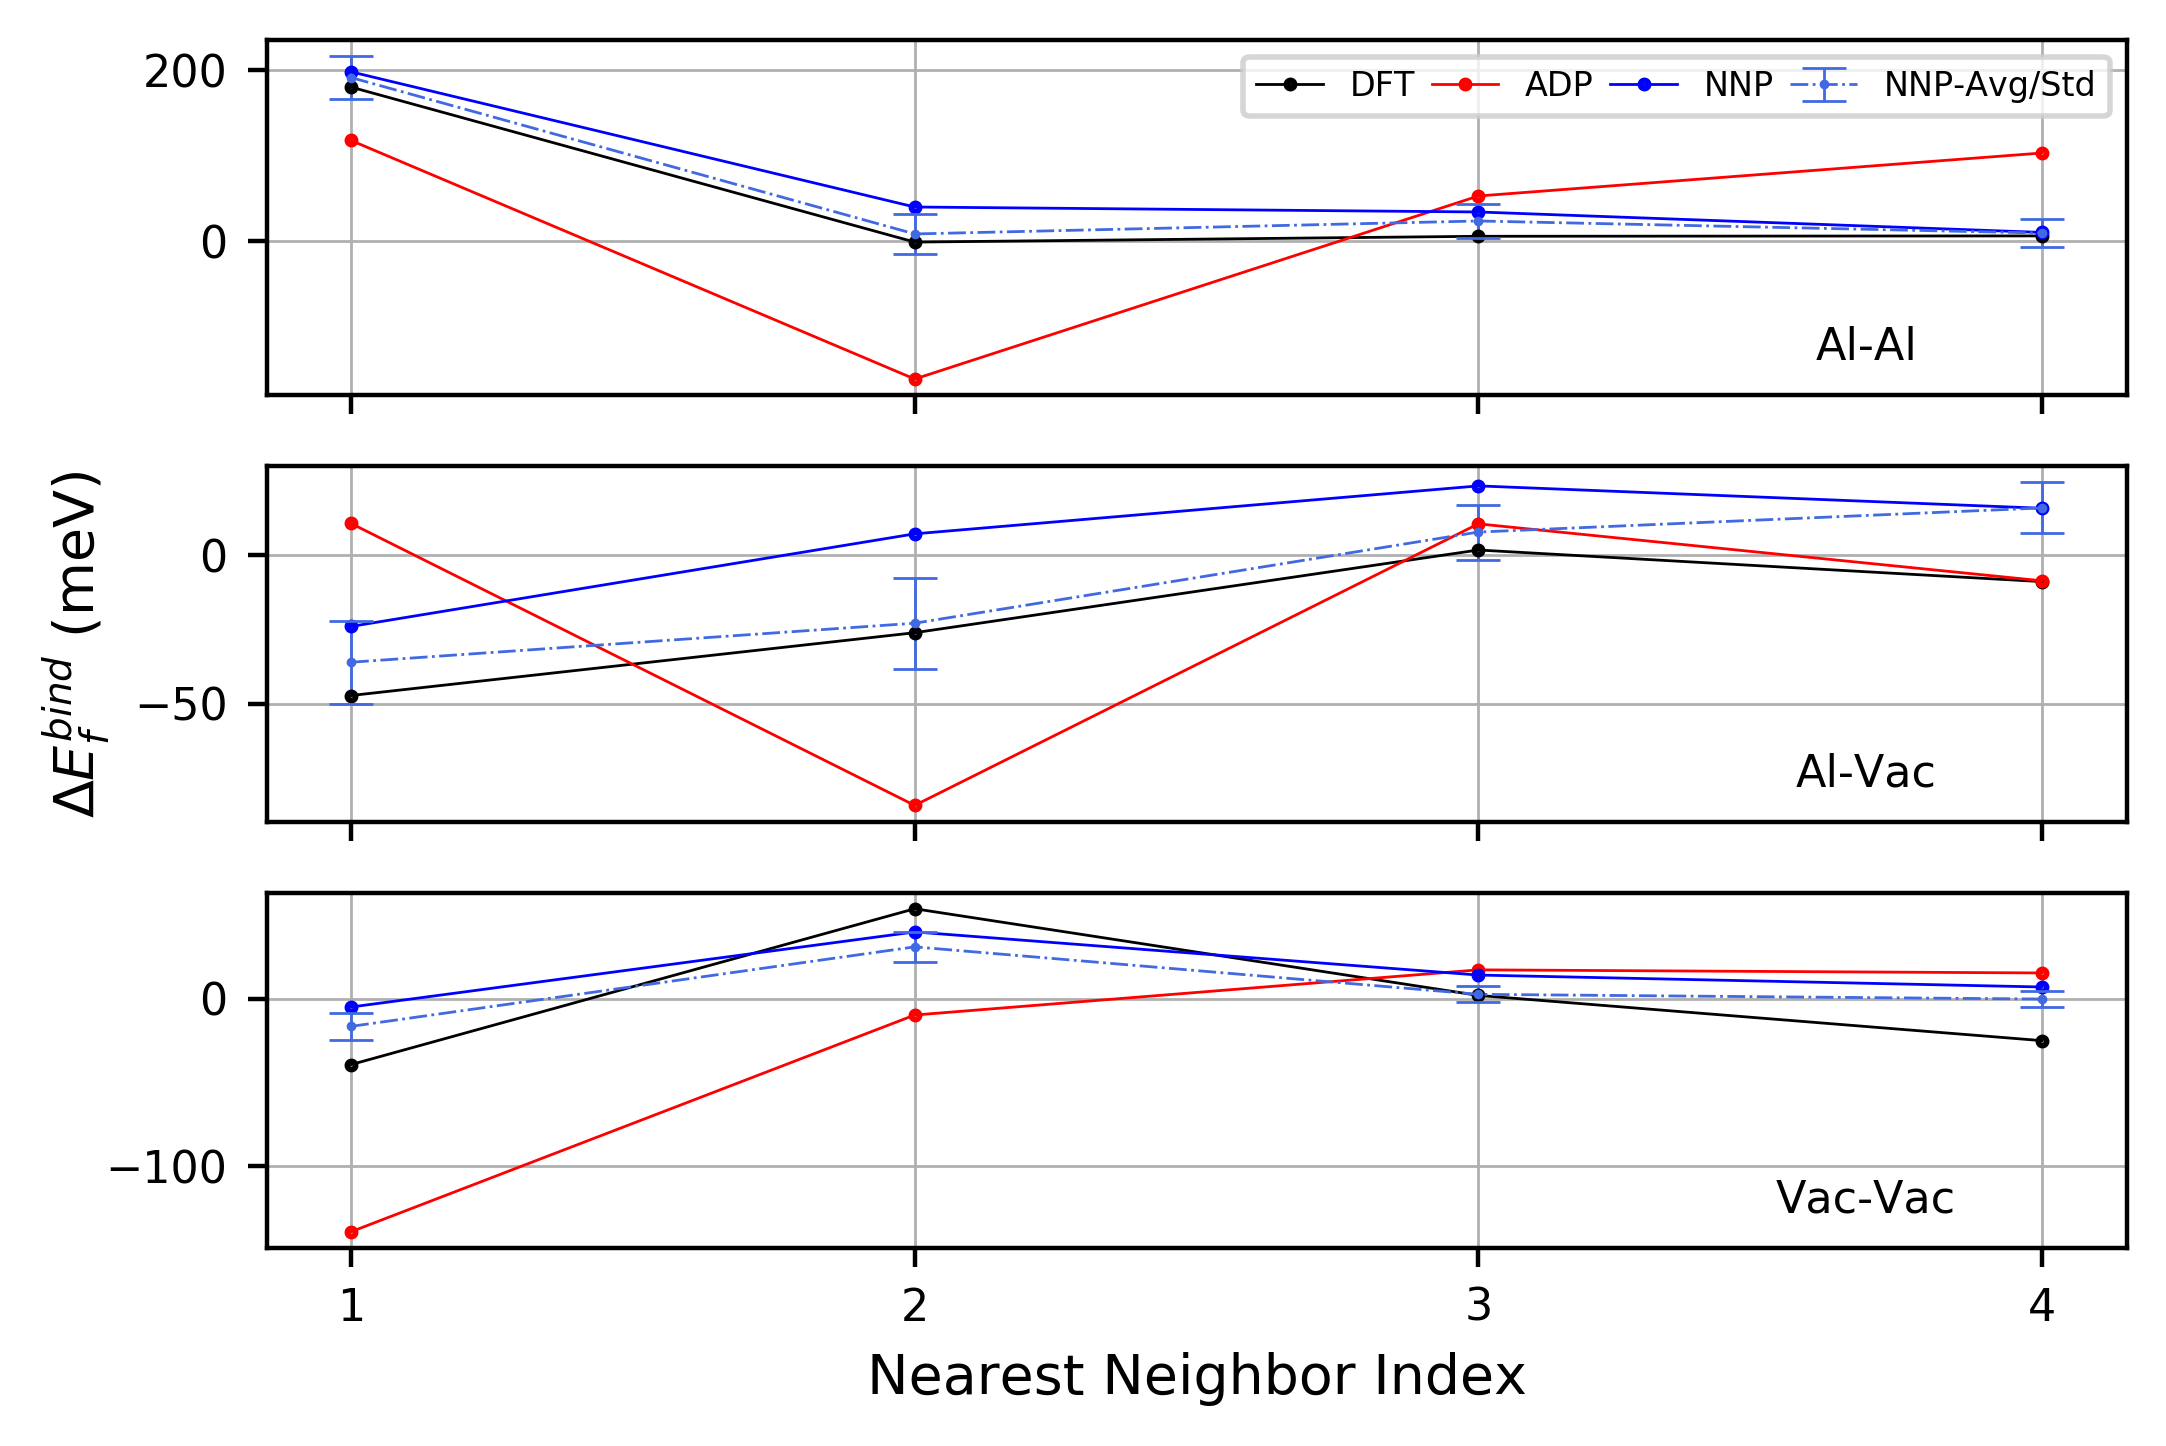
\includegraphics[width=1\textwidth,center]{./figures/solsol_in_cu.png}%
\caption{Neighbor index vs. binding energy $E_{bind}$ for Al-Al, Al-Vac and Vac-Vac in Cu matrix.}%
\label{fig:solsol_in_cu}
\end{figure}

\subsection{Additional Antisite Figures} \label{apd_sct:adn_antisites}
\begin{figure}[H]%
\centering%
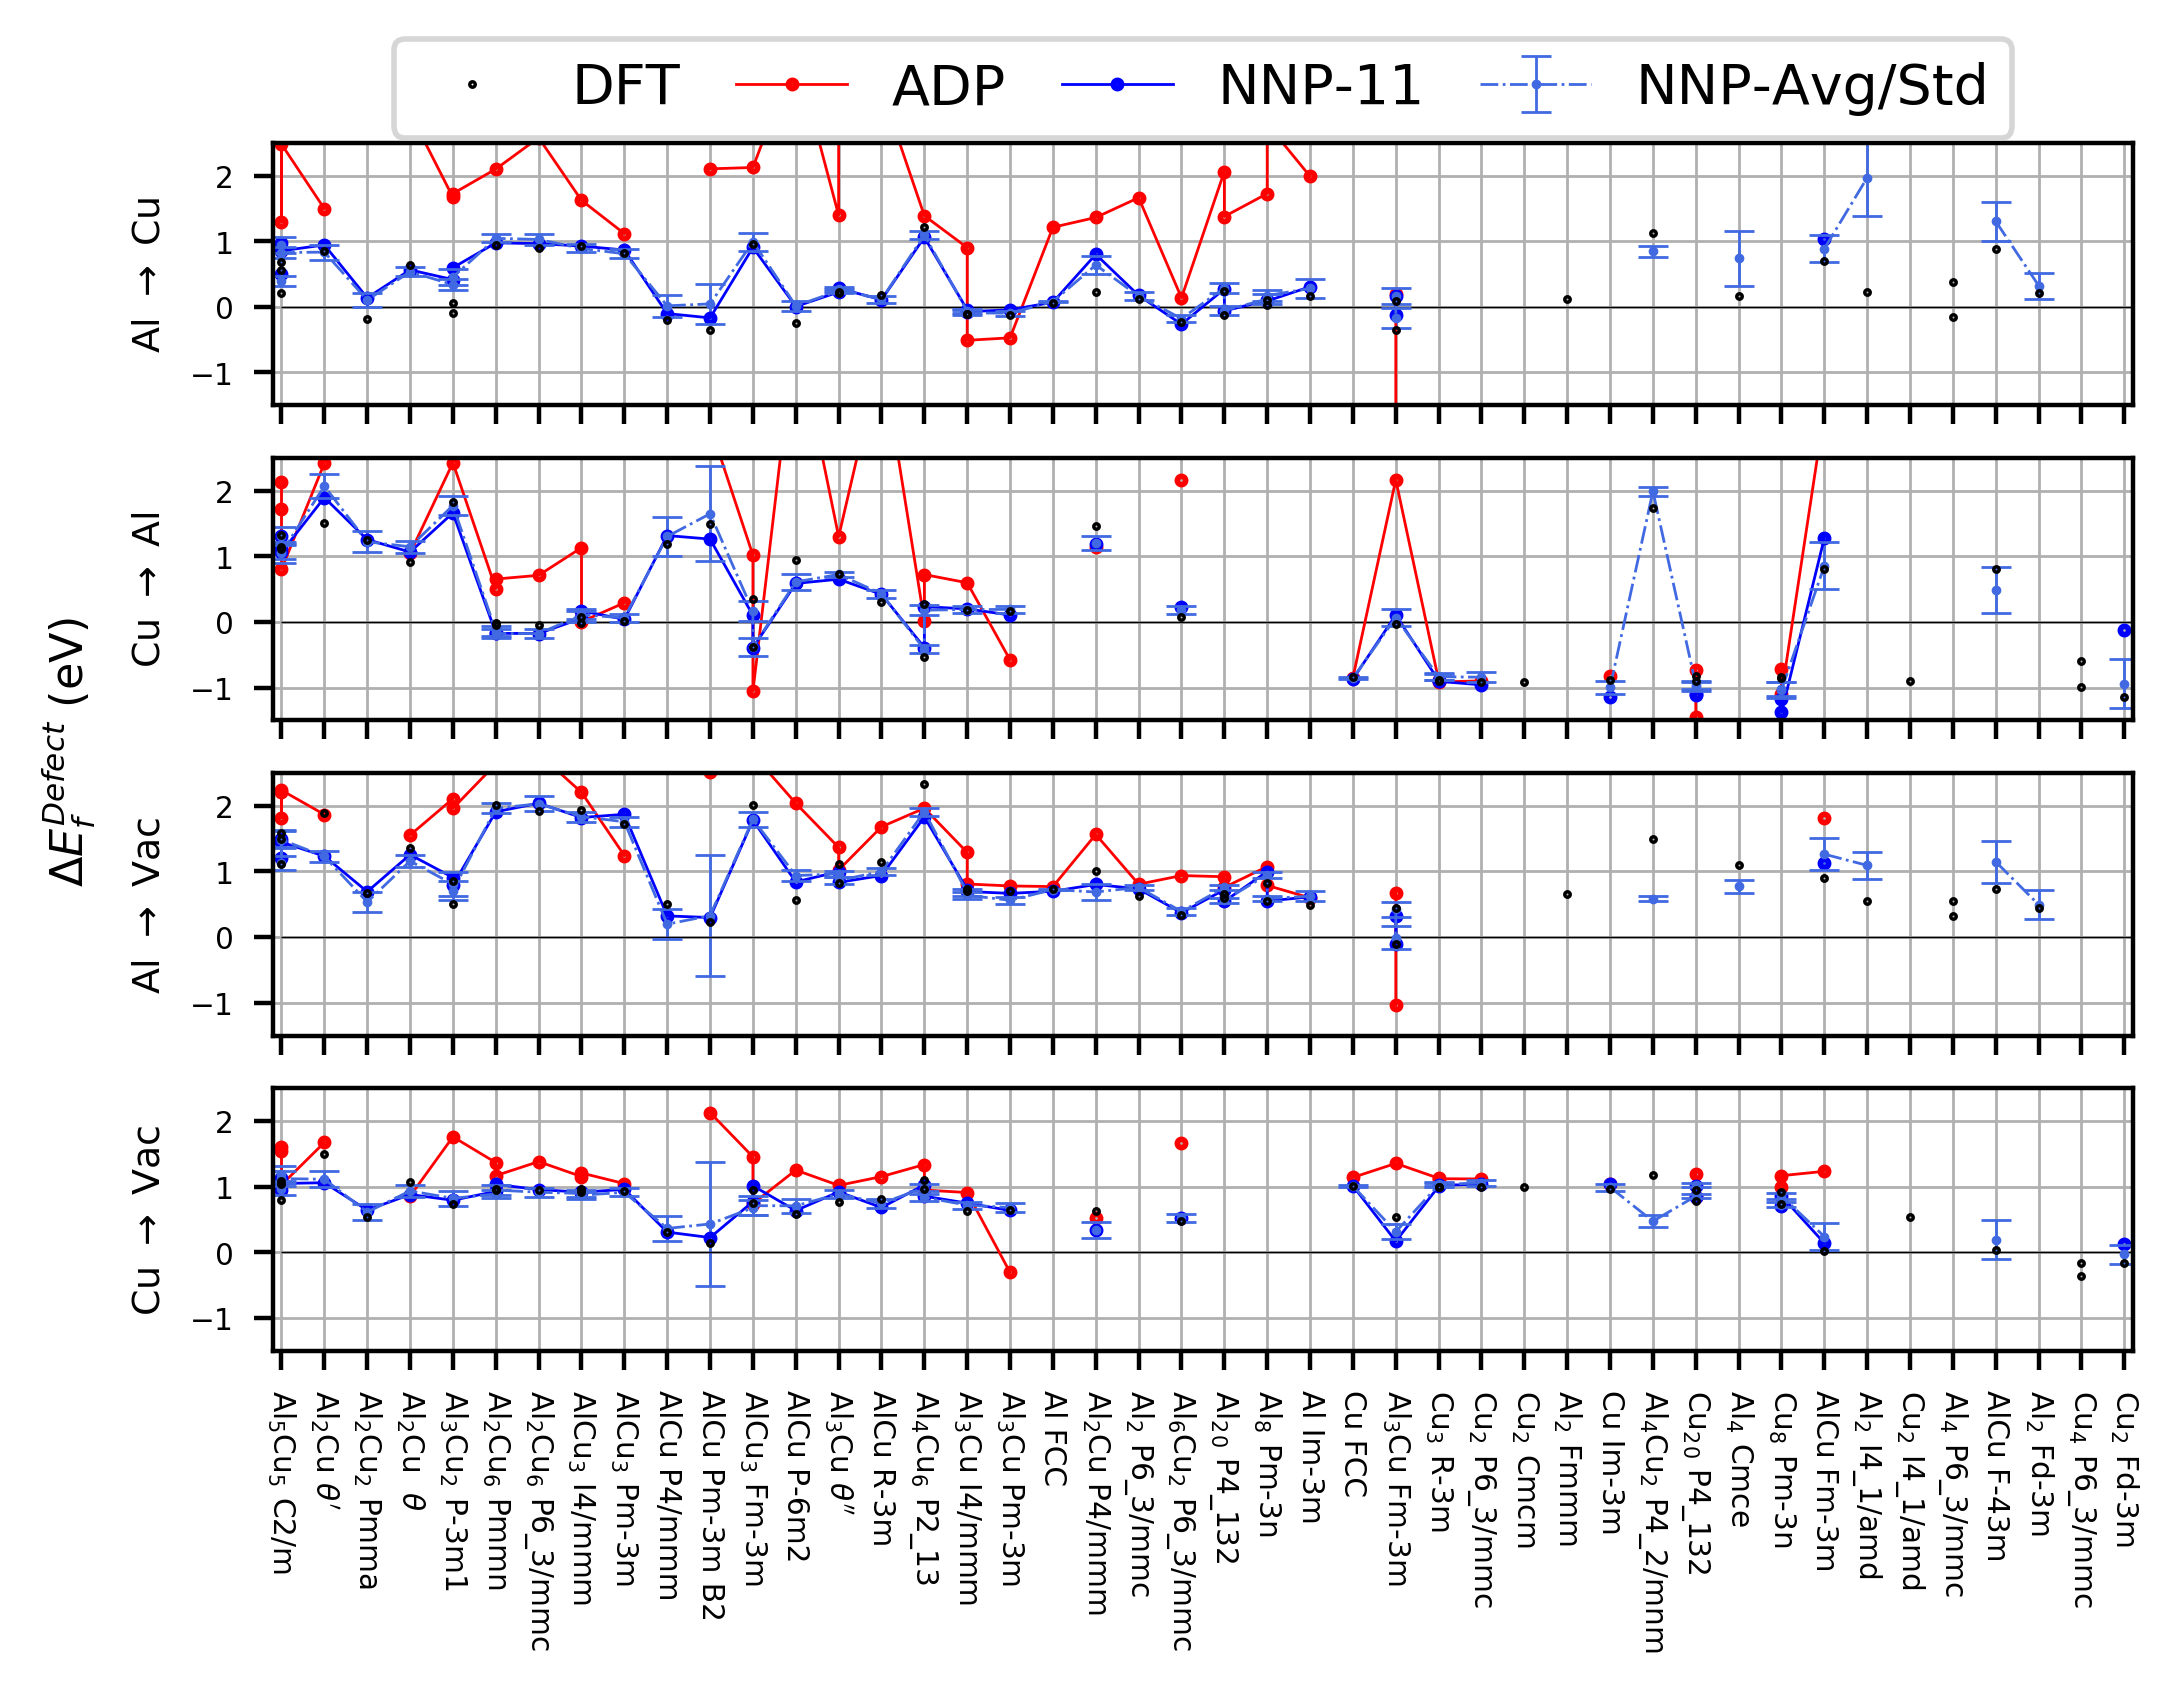
\includegraphics[width=1\textwidth,center]{figures/antisite_vacancies_allsites.png}%
\caption{DFT antisite formation energy vs. ADP/NNP antisite formation energy
for all vacancies and antisites.
These structures were not included in the training set.}%
\label{fig:antisite_plot_all}
\end{figure}

\subsection{Dislocations and Fracture} \label{apd_sct:fracturedislocation_images}


\begin{figure}[H]%
\centering%
\subfloat[]{{
 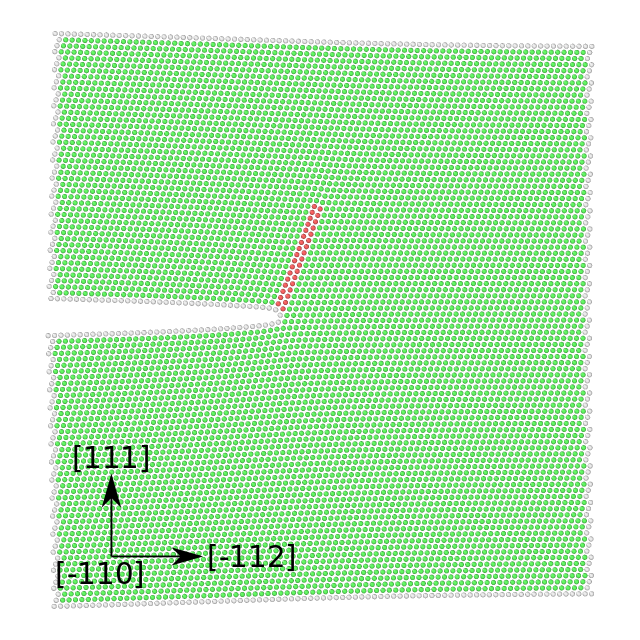
\includegraphics[width=0.50\textwidth]{figures/fracture_emit-leading.png}
 }}%
\subfloat[]{{
 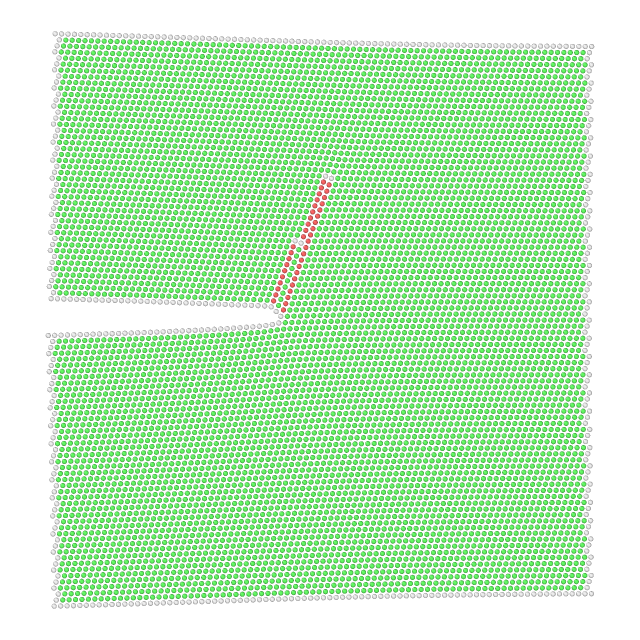
\includegraphics[width=0.50\textwidth]{figures/fracture_emit-leading-twin.png}
 }}%
\\
\caption{Observed dislocation emissions: (a) Leading (b) Leading and Twin Partial.
Green atoms are those in FCC configuration, red are for HCP (i.e. stacking faults) and white atoms are neither HCP nor FCC (e.g. surfaces, crack tips).}
\label{fig:fracturedislocation_images}
\end{figure}




\subsection{Additional Tables}
\begin{tabular}{l|lll|lll}%
\hline%
Structure&\multicolumn{3}{c}{FCC Al}&\multicolumn{3}{c}{FCC Cu}\\%
Method&DFT&NNP11&ADP&DFT&NNP11&ADP\\%
\hline%
a ($\AA$)&4.04&4.047&4.05&3.625&3.627&3.615\\%
vol/atom ($\AA^3$)&16.48&16.58&16.61&11.9&11.93&11.81\\%
G (GPa)&30.7&33.0&29.6&59.4&62.6&55.3\\%
K (GPa)&78.2&77.2&78.5&143.9&146.3&138.9\\%
$C_{11}$ (GPa)&112.5&110.6&113.5&180.3&182.4&170.4\\%
$C_{21}$ (GPa)&61.0&60.5&61.1&125.7&128.2&123.2\\%
$C_{44}$ (GPa)&34.0&38.2&31.9&80.8&86.3&76.5\\%
\hline%
\end{tabular}%
\newline%
\newline%
\newline%
\newline%

\begin{tabular}{l|ccc|ccc|ccc}%
\hline%
Structure&\multicolumn{3}{c}{Al$_2$Cu  $\theta$}&\multicolumn{3}{c}{Al$_2$Cu $\theta'$}&\multicolumn{3}{c}{Al$_3$Cu $\theta''$}\\%
Method&DFT&NNP11&ADP&DFT&NNP11&ADP&DFT&NNP11&ADP\\%
\hline%
a ($\AA$)&4.869&4.917&4.862&4.087&4.095&3.994&2.804&2.792&2.784\\%
b ($\AA$)&4.926&4.929&4.862&4.087&4.095&3.994&2.804&2.792&2.784\\%
c ($\AA$)&4.926&4.929&4.862&4.087&4.095&3.994&7.65&7.65&7.586\\%
$\alpha$&75.9&75.6&75.2&60.0&60.0&60.0&90.0&90.0&90.0\\%
$\beta$&60.4&60.1&75.2&60.0&60.0&60.0&90.0&90.0&90.0\\%
$\gamma$&60.4&60.1&60.6&60.0&60.0&60.0&90.0&90.0&90.0\\%
vol/atom ($\AA^3$)&14.88&14.95&14.41&16.09&16.18&15.02&15.04&14.9&14.69\\%
$\Delta$$H^{comp}$ (meV/atom)&{-}161.6&{-}162.9&{-}189.8&{-}184.0&{-}184.0&{-}202.6&{-}94.2&{-}94.8&{-}128.8\\%
G (GPa)&42.3&39.3&57.5&56.6&56.5&44.1&48.8&40.6&32.6\\%
K (GPa)&100.8&115.7&154.5&97.0&96.8&138.6&94.3&89.5&84.9\\%
$C_{11}$ (GPa)&170.4&167.8&199.5&158.7&160.4&192.4&160.5&148.6&115.4\\%
$C_{22}$ (GPa)&170.4&167.8&199.5&158.7&160.4&192.4&160.5&148.6&115.4\\%
$C_{33}$ (GPa)&174.8&180.4&278.2&158.7&160.4&192.4&181.8&154.1&142.0\\%
$C_{44}$ (GPa)&28.8&37.0&80.0&63.5&62.3&46.5&45.8&32.4&38.2\\%
$C_{55}$ (GPa)&28.8&37.0&80.0&63.5&62.3&46.5&45.8&32.4&38.2\\%
$C_{66}$ (GPa)&47.5&38.1&21.0&63.5&62.3&46.5&42.2&46.6&27.4\\%
$C_{21}$ (GPa)&73.7&104.2&99.3&66.2&64.9&111.6&70.9&61.6&48.0\\%
$C_{31}$ (GPa)&61.1&79.2&128.7&66.2&64.9&111.6&51.1&57.6&73.8\\%
$C_{32}$ (GPa)&61.1&79.2&128.7&66.2&64.9&111.6&51.1&57.6&73.8\\%
\hline%
\end{tabular}%






\end{document}
